\documentclass[a4paper]{report}
\usepackage{float}
\usepackage{verbatim}
\usepackage[utf8]{inputenc}
\usepackage[italian]{babel}
\usepackage{amsmath}
\usepackage{amsbsy,amssymb,amsfonts, amsthm, mhchem, multicol}
\usepackage{graphicx}
\usepackage[left=2cm,right=2cm,top=2cm,bottom=2cm]{geometry}
\usepackage{xcolor}
\usepackage[hypertexnames=false]{hyperref}
\usepackage{nameref}
\usepackage{framed}
\usepackage[framemethod=TikZ]{mdframed}

% figure support
\usepackage{import}
\usepackage{xifthen}
\pdfminorversion=7
\usepackage{pdfpages}
\usepackage{transparent}
\newcommand{\incfig}[1]{%
	\def\svgwidth{\columnwidth}
	\import{./figures/}{#1.pdf_tex}
}
\newcommand{\ffrac}[2]{\ensuremath{\frac{\displaystyle #1}{\displaystyle #2}}}
\newcommand{\angstrom}{\mbox{\normalfont\AA}}
\newcommand{\bs}{\boldsymbol}
\renewcommand{\[}{\begin{equation}}
\renewcommand{\]}{\end{equation}}
\renewcommand{\theequation}{\thesection.\arabic{equation}}
\counterwithin*{equation}{section}

% title setup
\makeatother
\def\@lez{}%
\newcommand{\lez}[3]{
    \ifthenelse{\isempty{#3}}{%
        \def\@lez{Lezione #1}%
    }{%
        \def\@lez{Lezione #1: #3}%
    }%
    \section{\@lez}
    \marginpar{\small\textsf{\mbox{#2}}}
}
\makeatletter

%fatto
\newcounter{fact}[section]\setcounter{fact}{0}
\renewcommand{\thefact}{\arabic{section}.\arabic{fact}}
\newenvironment{fact}[2][]{%
\refstepcounter{fact}%
\ifstrempty{#1}%
{\mdfsetup{%
frametitle={%
\tikz[baseline=(current bounding box.east),outer sep=0pt]
\node[anchor=east,rectangle,fill=blue!20]
{\strut Fatto~\thefact};}}
}%
{\mdfsetup{%
frametitle={%
\tikz[baseline=(current bounding box.east),outer sep=0pt]
\node[anchor=east,rectangle,fill=blue!20]
{\strut Fatto~\thefact:~#1};}}%
}%
\mdfsetup{innertopmargin=10pt,linecolor=blue!20,%
linewidth=2pt,topline=true,%
frametitleaboveskip=\dimexpr-\ht\strutbox\relax
}
\begin{mdframed}[]\relax%
\label{#2}}{\end{mdframed}}

%definizione
\newcounter{defn}[section]\setcounter{defn}{0}
\renewcommand{\thedefn}{\arabic{section}.\arabic{defn}}
\newenvironment{defn}[2][]{%
\refstepcounter{defn}%
\ifstrempty{#1}%
{\mdfsetup{%
frametitle={%
\tikz[baseline=(current bounding box.east),outer sep=0pt]
\node[anchor=east,rectangle,fill=green!20]
{\strut Definizione~\thedefn};}}
}%
{\mdfsetup{%
frametitle={%
\tikz[baseline=(current bounding box.east),outer sep=0pt]
\node[anchor=east,rectangle,fill=green!20]
{\strut Definizione~\thedefn:~#1};}}%
}%
\mdfsetup{innertopmargin=10pt,linecolor=green!20,%
linewidth=2pt,topline=true,%
frametitleaboveskip=\dimexpr-\ht\strutbox\relax
}
\begin{mdframed}[]\relax%
\label{#2}}{\end{mdframed}}


\author{Edoardo Gabrielli}
\title{Appunti di astrofisica}

\begin{document}
\maketitle
\clearpage
\tableofcontents
%\clearpage
\chapter{Introduzione e Trasporto Radiativo}
%\lez{1}{20-02-2020}{}
\subsubsection{Introduzione}%
Il corso è di astrofisica generale e darà una infarinatura generale degli argomenti principali dell'astrofisica.
\paragraph{Libro di testo}%
\texttt{Astrophysics for Physicists, Arnab Rai Choudhri}
\paragraph{Argomenti del corso}%
\begin{itemize}
	\item Trasporto radiativo.
	\item Stelle.
	\item Aggregati di stelle.
	\item Mezzo interstellare.
	\item Ammassi di galassie.
\end{itemize}
\subsection{Osservazione del cielo}%
\paragraph{Astrofisica}%
L'astrofisica è una scienza osservativa: non possiamo decidere di modificare il nostro "apparato", possiamo solo soltanto raccogliere informazioni attraverso le tecnologie di osservazione che abbiamo.\\
Le informazioni possono essere raccolte attraverso i diversi tipi di \textbf{messaggeri} che ci arrivano dal cosmo.\\
Il messaggero principale è la radiazione elettromagnetica, ultimamente si sono aggiunti altri portatori di informazioni: prima le particelle (neutrini) e successivamente le onde gravitazionali.\\ 
Resta il fatto che la stragrande maggioranza di informazioni che sappiamo dall'universo proviene dalla radiazione elettromagnetica.\\ 
Non potendo decidere quando i fenomeni avvengono sarà necessario sviluppare delle strategie che permettano di avere una sorta di \texttt{ridondanza osservativa} per riuscire ad accertare un supposto evento.

\paragraph{Osservazione della radiazione elettromagnetica}%
Fino all seconda guerra mondiale si osservava soltanto nella fascia dello spettro del visibile: tra i 4000 ed i 7000 \AA.\\
Successivamente, grazie all'invenzione del radar si sono aperte le regioni del Radio, X, Infrarosso, Gamma. Oggi si fanno osservazioni in tutto lo spettro. 

\paragraph{Lotta contro l'oscurità}%
La sfida è sempre stata nel vedere sorgenti deboli. Una sorgente può essere debole perchè è intrinsecamente debole (nana bianca antichissima, pianeti) oppure sorgenti intrinsecamente molto luminosi ma molto molto lontani. \\
Poter osservare oggetti sempre più lontani significa aumentare il numero di osservazione: posso avere più possibilità di osservare fenomeni mai visti prima e fare nuova fisica.\\
Per vedere oggetti sempre meno luminosi abbiamo bisogno di lenti dei telescopi sempre più grandi. Attualmente i telescopi ottici più grandi hanno diametri di 10 metri. L'ESA sta costruendo un telescopio di diametro di 39 metri. Avere un diametro più grande significa avere una sensibilità maggiore.

\subsection{Diffrazione e Seeing}%
\paragraph{Telescopi sempre più grandi}%
Aumentando la superficie della lente del telescopio aumenta la capacità di catturare luce e quindi la sensibilità del telescopio. Tuttavia questo non è l'unico motivo per cui si costruiscono telescopi sempre più grandi: c'è anche un motivo legato alla risoluzione del telescopio.\\
Quando guardiamo il cielo noi osserviamo degli angoli, le varie sorgenti che sono proiettate sulla volta celeste. La risoluzione è l'angolo più piccolo tra due sorgenti proiettate sulla volta celeste che mi permette di distinguerle.\\
Infatti per le dimensioni angolari degli oggetti luminosi nel cielo non sono trascurabili effetti di diffrazione. 
\paragraph{Diffrazione}%
Prendiamo il classico problema della fenditura:
\begin{figure}[H]
    \centering
    \incfig{diffrazione-da-una-fenditura}
    \caption{Diffrazione da una fenditura}
    \label{fig:diffrazione-da-una-fenditura}
\end{figure}
\noindent
Sappiamo che gli zeri della funzione di intensità $\frac{I}{I_0}$ sono nei punti:
\[
	\sin\theta = \frac{\lambda}{D}\cdot m \quad \quad m \text{ intero}
.\] 
Con il nostro telescopio abbiamo una situazione simile: abbiamo una stella lontana che irraggia. La sua luce entra in una fenditura circolare di diametro D data dal telescopio. Per il principio di Babinet sappiamo che anche in questo caso si crea una figura di interferenza che prenderà la seguente forma:
\begin{figure}[H]
	\centering
	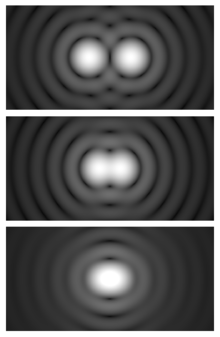
\includegraphics[width=0.2\textwidth]{figures/diffraction.png}
	\caption{\scriptsize Diffrazione al telescopio per due stelle al variare della risoluzione angolare.}
	\label{fig:diffraction}
\end{figure}
\noindent
Questa struttura di rifrazione ci permette di ridefinire il concetto di risoluzione, questa volta gli zeri sono in corrispondenza di alcuni numeri, il primo zero va ha $m=1.22$. \\
Il cerchio centrale, detto disco di Airy è importante perchè ci permette di discriminare due oggetti, questo risulta evidente in \hyperref[fig:diffraction]{Figura 2}\\
Prendendo angoli progressivamente più piccoli le figure di diffrazione tengono a sovrapporsi, il criterio per dire quando due sorgenti sono distinguibili è detto Criterio di Rayleigh: due sorgenti si dicono distinte quando hanno dischi di Hairy con centri che giacciono uno all'esterno dell'altro.
Quindi l'angolo minimo che riesco a risolvere sarà: 
\[
	\sin\theta_{min} \approx \theta_{min} =  1.22 \frac{\lambda}{D}
.\]
Quindi la risoluzione angolare di questo telescopio è data da questa formula. Per questo possiamo capire perchè è importante avere telescopi sempre più grandi.\\

Quando un telescopio arriva alla situazione in cui il limite di funzionamento è quello di diffrazione si dice che siamo nelle condizioni ottimali: quelle di Diffraction Limited (Hubble è in queste condizioni). 
\paragraph{Seeing}%
Sulla terra si può arrivare alla condizione ottimale del paragrafo precedente? In genere no per colpa della atmosfera, avente indice di diffrazione variabile è la maggiore fonte di disturbo.
\begin{figure}[H]
	\centering
	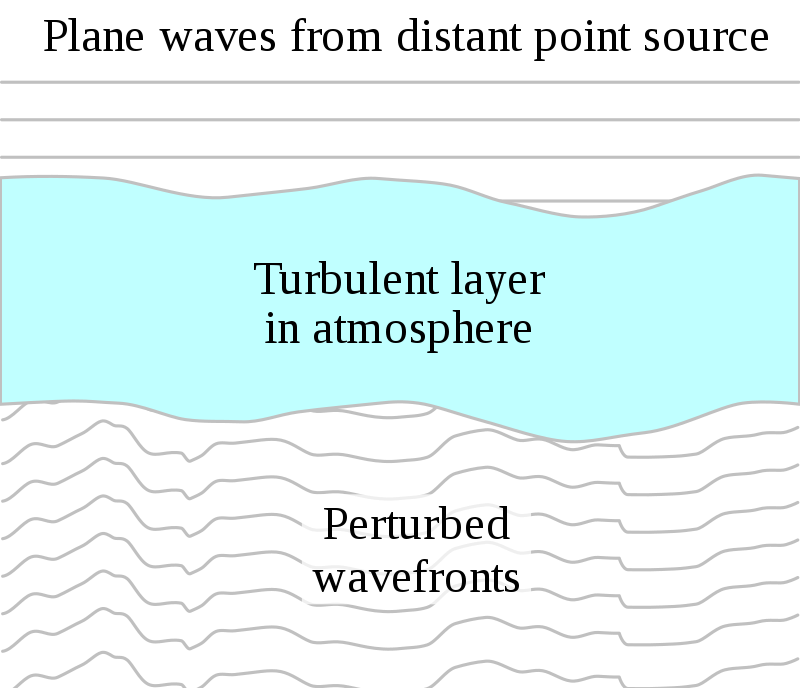
\includegraphics[width=0.3\textwidth]{figures/seeing.png}
	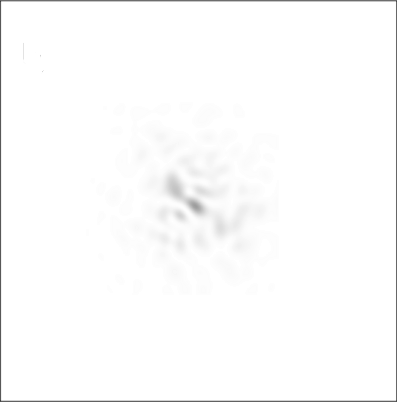
\includegraphics[width=0.2\textwidth]{figures/seeing-effect.png}
	\caption{\scriptsize A destra un possibile effetto sui fronti d'onda che attraversano l'atmosfera e a sinistra il risultato sulla stella agli occhi del telescopio, l'immagine risulta allargata e distorta.}
	\label{fig:figures-seeing-png}
\end{figure}
\noindent
Qual'è l'ordine di grandezza del Seeing? Se è buono si arriva al "secondo d'arco": $1''$. Nei siti migliori si arriva a $0.5''$.\\
Possiamo allora chiederci qual'è il valore del diametro del telescopio che mi produce un angolo di diffrazione minimo che corrisponde a quello del seeing. A quel punto non mi servirebbe a niente aumentare le dimensioni della lente: il seeing ci sarebbe comunque.\\
Nella luce visibile si ha $\lambda \approx 5000$ \AA, se prendiamo a questa lunghezza d'onda un angolo di $1''$ vediamo che il telescopio che raggiunge il limite del seeing è minuscolo: $D=$ 12 cm.\\
Perchè allora si costruiscono telescopi di 40 metri di diametro?
\begin{itemize}
	\item Per raccogliere comunque più luce.
	\item Per via dell'avvento della elettronica.
\end{itemize}
Esiste infatti un sistema detto ottica adattiva per correggere la presenza dell'atmosfera: si spara una sorgente laser in aria e si cercano di compensare elettronicamente l'effetto dell'atmosfera.
\paragraph{Lunghezza d'onda per cui oggi si ha la massima risoluzione angolare}%
Ha senso diminuire $\lambda$ fissando $D$, sembrerebbe quindi sensato andare nel Gamma, oggi invece si ha la risoluzione massima nel Radio grazie a Tecniche di interferometria: possiamo costruire array di telescopi che lavorano simultaneamente (si registra con orologi atomici l'arrivo del segnale): si arriva a  $D = 8600$ km (baseline molto lunga). Con questo metodo si arriva a risoluzioni di decine di micro arcosecondi! Questo è sicuramente il caso della foto del buco nero (30 arcosecondi). 
\begin{figure}[H]
	\centering
	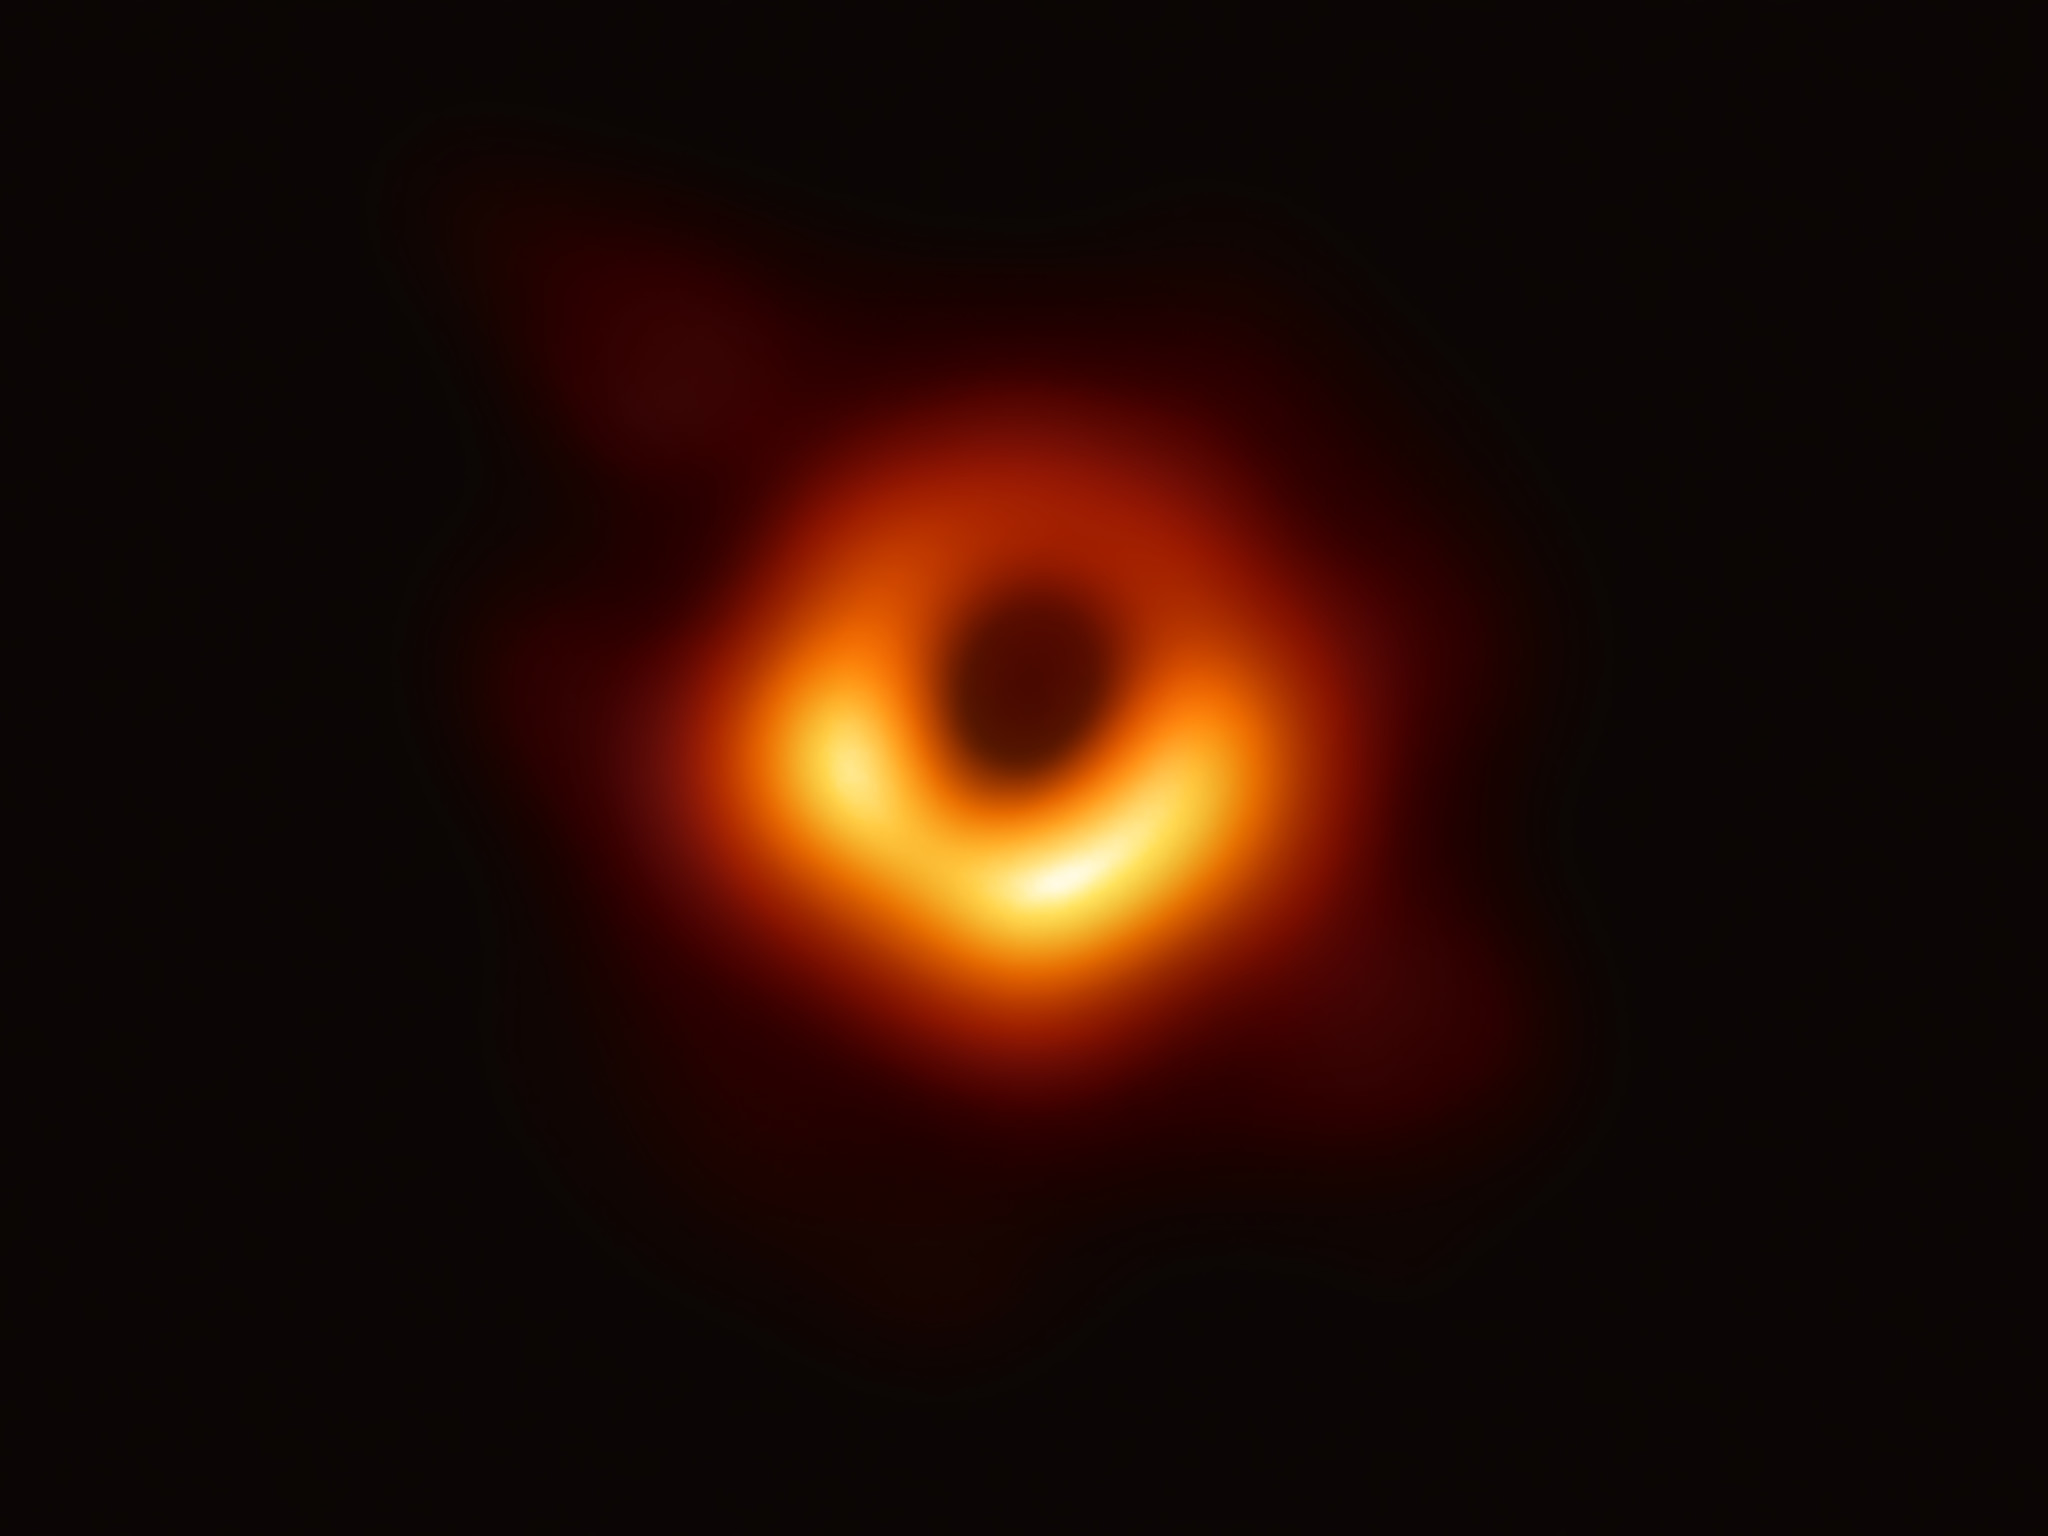
\includegraphics[width=0.4\textwidth]{figures/buconeroimmagine.jpg}
	\caption{Immagine del buco nero raccolta nel 2019}
	\label{fig:figures-buconeroimmagine-jpg}
\end{figure}

Ci sono alcune grandezze in astrofisica che non possono essere dimenticate ai fini di comprendere le grandezze di cui stiamo parlando. Queste grandezze alcune volte vengono anche adottate come unità di misura, visto che nella scala astrofisica le unità standard ridulterebbero decisamente incomprensibili!\\

\subsection{Massa del sole}%
Massa del sole: M\textsubscript{\(\odot\)} = $1.989 \cdot 10^{33}$ g $\approx 2 \cdot 10^{33} g$.\\
La massa minima per una stella è circa 0.08 M\textsubscript{\(\odot\)}\footnote{questa è la massa minima per innescare le reazioni termonucleari, chi non raggiunge queste dimensini (ma si avvicina) è detta Nana Bruna}, la massima si aggira attorno a 100 M\textsubscript{\(\odot\)}. \\
Le galassie hanno circa $10^{11}$ stelle, da cui per ottenere la massa di queste ultime si può mediare la massa a quella del sole con l'adeguato esponente. \\
Abbiamo anche aggregati di stelle (tipo Pleiadi, migliaglia di stelle) e più in là vedremo e studieremo gli ammassi di galassie.

\subsection{Distanze e metodo della parallasse}%
Raggio del sole: $R_{\odot} \approx 7 \cdot 10^{10} cm$.\\
La misura delle distanze in astronomia è complicata. Sono necessarie misure indirette spesso. Se voglio conoscere le dimensioni fisiche di un oggetto (trasformare angolo in distanza) ho bisogno di sapere quanto è distante! 
\paragraph{Metodo della parallasse}%
È l'unica misura diretta di distanza disponibile. È inoltre una misura di tipo geometrico:
\begin{figure}[H]
    \centering
    \incfig{metodo-della-parallasse}
    \caption{\scriptsize Metodo della parallasse: la stella risulta in diversi punti del cielo a seconda della posizione della terra.}
    \label{fig:metodo-della-parallasse}
\end{figure}
\noindent
Negli anni novanta abbiamo mandato un satellite che misurava fino ad un millesimo di secondo d'arco. La missione attuale più importante al riguardo è la GAIA: sta adesso mappando il cielo, quando tra qualche anno avrà finito si arriva a 30 microarcosecondi, purtoppo non si esce ancora dalla galassia con questo metodo.\\
Il metodo consiste in pratica nel vedere lo spostamento angolare dell'oggetto in momenti diversi dell'orbita di rotazione della terra attorno al sole: l'angolo di parallasse $\pi$ è la metà dell'angolo $\theta$
\[
	\frac{\theta}{2} = \pi
.\] 
Se conosciamo il raggio di orbita terrestre possiamo trovare la distanza della stella.\\
Noi conosciamo il raggio dell'orbita terreste medio \footnote{Grazie ad un trasponder radar montato sulla luna}, esso è l'unità astronomica A.U: $R \approx 1.5 \cdot 10^{13}$ cm.
\[
	\tan\left( \pi \right) \approx \pi  = \frac{R}{d}
.\] 

Il sistema solare (fino a nettuno) abbiamo una dimensione di 30 A.U. Fuori dal sistema solare è necessario definire un'altra unità di misura: il Parsec.\\
Un parsec è una distanza tale che la parallasse annua è 1'':
\[
	1 \text{ pc} \approx 3.09 \cdot 10^{18} \text{ cm} \sim 3.2 \text{ anni luce}
.\] 
La stella più vicina a noi ha una parallasse annua di 0.75'' l'anno (Proxima Centauri) che equivale a 1.3 pc. Misurare questi angoli è difficile in generale, gli angoli sono molto piccoli.\\
Le dimensioni di una galassia come la nostra invece sono:\\
\begin{figure}[H]
	\centering
	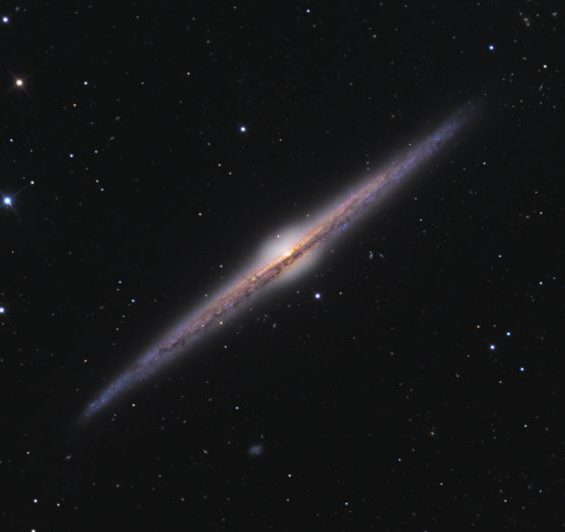
\includegraphics[width=0.4\textwidth]{figures/vialattea.jpeg}
	\caption{Rendering della via lattea vista dall'esterno.}
	\label{fig:figures-vialattea-jpeg}
\end{figure}
\[
	R_{disco} \sim 15 k\text{pc}
.\]
La distanza tra le galassie più vicine tra loro è dell'ordine del Mpc.\\
In genere le stelle invece distano tra loro di quantità dell'ordine dei parsec, è raro che collidano tra loro: l'una tra l'altra sono molto lontane rispetto alle dimensioni delle stelle stesse.\\ 
Non si può dire lo stesso per le galassie, ci sono solo pochi ordini di grandezza tra il raggio galattico è la distanza tra una galassia e l'altra, infatti le collisioni tra galassie sono più frequenti.\\
Le galassie più distanti sono dell'ordine del Gpc (questa è anche la scala delle dimensioni dell'universo).\\
\begin{figure}[H]
    \centering
    \incfig{scale-dell'universo}
    \caption{\scriptsize Scale dell'universo, il disegno è schematico e non è ovviamente in scala.}
    \label{fig:scale-dell'universo}
\end{figure}
\noindent

\subsection{Scale temporali dell'universo}%
Età del sole: $T_{\odot} = 4.57$ Gyr (Giga year). Questa è una delle poche datazioni misurata in modo diretto in astronomia, questa deriva dallo studio delle comete: queste sono rimaste intatte per miliardi di anni, queste vengono datate attraverso radiodatazioni.\\
Età dell'universo (dal Big Bang ad oggi): $T_{uni}= 13.8$ Gyr.

\subsection{Luminosità intrinseca, Candele campioni ed introduzione al trasporto radiativo}%
Negli anni '90 l'ESA ha mandato un satellite in grado di mappare decine di migliaglia di stelle attorno a noi distanti fino a 10 pc. GAIA è l'evoluzione di questo progetto, essa permettera di mappare tridimensionalmente la galassia. \\
Tuttavia anche con GAIA non si esce dalla galassia, quindi come si fa ad uscire? Come si misura la distanza se non sono in grado di misurare la parallasse?\\
Serve un metodo indiretto basato sul'concetto di \texttt{Candela campione}: un oggetto astronomico ci cui conosco la luminosità intrinseca.\\
Confrontando la luminosità intrinseca e la luminosità apparente osservata possiamo dedurre la distanza dell'oggetto. Questo è l'unico modo per misurare le distanze di oggetti all'esterno della via lattea. (Gli oggetti campione sono in genere le supernove).\\
Come faccio a partire dalla luminosità intrinseca a misurare la distanza?
\begin{figure}[H]
    \centering
    \incfig{propagazione-della-radiazione}
    \caption{Propagazione della radiazione}
    \label{fig:propagazione-della-radiazione}
\end{figure}
\noindent
Prendiamo una sorgente che irraggia come in \hyperref[fig:propagazione-della-radiazione]{Figura 8}. 
Se chiamiamo $F\left( r_1 \right) $ il flusso della radiazione che attraversa la superficie sferica concentrica alla sorgente di raggio $r_1$ allora:
\[
	F\left( r_1 \right) 4\pi r_1^2 = F\left( r_2 \right) 4\pi r_2^2 \implies F\left( r_2 \right) = F\left( r_1 \right) \left( \frac{r_1}{r_2} \right) ^2
.\] 
Abbiamo quindi una buona definizione di luminosità se ci mettiamo sul raggio $R$ della stella che irraggia:
\[
	F\left( R \right) 4\pi R^2  = L
.\] 
Tuttavia questa a livello pratico non è sufficiente. La radiazione non si propaga nel vuoto, è indispensabile quindi costruire una teoria del trasporto radiativo per tener di conto del mezzo interstellare. \\
Dobbiamo introdurre alcune grandezze per studiare il trasporto radiativo: \texttt{Intensità specifica monocromatica} (trattata dal punto di vista macroscopico \footnote{Valido quando la lunghezza d'onda che stiamo studiando sono piccole rispetto alle dimensioni del sistema, questo ci permette di immaginare che la radiazione si propaghi lungo dei raggi}):
\begin{figure}[H]
    \centering
    \incfig{figura-per-introdurre-lintensit-specifica}
    \caption{Figura per introdurre l'intensità specifica}
    \label{fig:figura-per-introdurre-lintensit-specifica}
\end{figure}
\noindent
Supponiamo di essere in un punto $\bs{r}$ all'istante $t$ e prendiamo in questo punto una superficie infinitesima elementare $dA$ orientata nella direzione $\hat{n}$ come in \hyperref[fig:figura-per-introdurre-lintensit-specifica]{Figura 9}. Ci interessa calcolare l'energia trasportata dalla radiazione elettromagnetica che attraversa la superficie $dA$ nella direzione $\hat{k}$ all'interno dell'angolo solido $d\Omega$ (inoltre deve essere monocromatica: tra $\nu$ e $d\nu$).\\
Quello che cerchiamo è dato da:
\[
	dE = I_{\nu}\left( \bs{r}, t,\bs{k} \right) \hat{k}\hat{n} dAdtd\Omega d\nu
	= I_{\nu}\left( \bs{r},t, \bs{k} \right) \cos\theta dA dt d\Omega d\nu
.\] 
Questa quantità è un flusso per unità di angolo solito: una brillanza superficiale. 
\[
	[I_{v}] = \text{[erg] cm $^{-2}$ s $^{-1}$ ster $^{-1}$ Hz $^{-1}$} 
.\] 
Dove ster è lo ster radiante.\\
$I_{\nu}$ è l'energia trasportata da un gruppo di fotoni che si muovono tutti nella stessa direzione contemporaneamente e tutti con la stessa frequenza.\\
È necessario notare che l'interazione tra radiazione e materia è anche argomento microscopico: il fotone interagisce anche con ioni, protoni, nuclei nel suo tragitto. Terremo conto con opportuni coefficienti il passaggio della radiazione nei vari mezzi quando scriveremo l'equazione del trasporto.\\

%\lez{2}{24-02-2020}{}
Riprendiamo la teoria del trasporto radiativo.
\[
	dE = I_{\nu}\left( \bs{r}, t,\bs{k} \right) \hat{k}\hat{n} dAdtd\Omega d\nu
.\] 
Conoscere il campo di radiazione in una determinata regione significa conoscere l'intensità specifica del campo di radiazione: $I_{\nu}\left( \bs{r}, t,\bs{k} \right)$.\\ 
Tale quantità ricordiamo essere un flusso per unità di angolo solido. Presa una superficie infinitesima dA come nella lezione precedente:
\begin{figure}[H]
    \centering
    \incfig{figura-per-introdurre-lintensit-specifica}
    \caption{Figura per introdurre l'intensità specifica}
    \label{fig:figura-per-introdurre-lintensit-specifica}
\end{figure}
\noindent
L'energia trasportata dalla radiazione elettromagnetica tra la frequenza $\nu$ e $\nu + d\nu$ che attraversa la superficie $dA$ è data dalla relazione con cui abbiamo introdotto questa lezione.\\
Questa $I_{\nu}\left( \bs{r}, t, \bs{k} \right)$ non descrive completamente il campo di radiazione: lo descrive nei confini dell'ottica geometrica. No tiene di conto infatti di fenomeni come interferenza e diffrazione. Anticipiamo che nella maggior parte delle situazioni di interesse la quantità $I_{\nu}\left( \bs{r}, t,\bs{k} \right)$ non dipende dal tempo perchè il campo di radiazione ed il mezzo stesso sono in genere stazionari \footnote{Ci sono anche casi in cui questo non è vero, nei casi che affrontiamo noi invece lo daremo per scontato.}. \\
\subsection{Momenti dell'intensità $I_{\nu}$}%
Spesso inoltre non serve conoscere direttamente  $I_{\nu}\left( \bs{r}, t,\bs{k} \right)$, bastano altre quantità con meno informazioni. Facciamo in questa sezione alcuni esempi.
\paragraph{Flusso}%
Immaginiamo di volere il flusso  $F_{\mu}$ monocromatico (tra la frequenza $\nu$ e $\nu + d\nu$) attraverso la superficie $dA$ nell'unità di tempo, calcoliamo dapprima la radiazione che si propaga nella direzione $\bs{k}$ che chiamiamo $\phi$:
\begin{align}
	\phi = \frac{\mbox{d} E}{\mbox{d} A \text{d}t} = \frac{I_{\nu}\cos\theta}{dA dt} dA dt d\Omega d\nu = I_{\nu} \cos\theta d\Omega d\nu
.\end{align}
Per ottenere il flusso basterà integrare in tutto l'angolo solido ottenendo:
\[
	F_{\nu} = \int_{\Omega} I_{\nu}\cos\theta d\Omega \ \left[ \text{erg} \right]  \left[ \text{cm} \right]^{-2} \left[ s \right]^{-1} \left[ \text{Hz} \right]^{-1} 
.\] 
Se vogliamo il flusso totale sarà necessario integrare nelle frequenze:
\[
	F = \int F_{\nu} d\nu
.\] 
Chiaramente nel flusso cè meno informazione che nella intensità specifica perchè abbiamo perso informazioni sull'angolo e quindi sulla direzione di propagazione.\\
Notiamo che nei casi in cui la radiazione è isotropa il flusso sarà nullo: la quantità di radiazione che va verso l'alto è la stessa di quella verso il basso \footnote{Infatti l'integrale fa proprio zero, poichè tutto esce dall'integrale in $\Omega$ tranne il coseno, mentre l'elemento infinitesimo di angolo solido è proporzionale a $\sin\theta d\theta$}.\\
Un esempio di radiazione isotropa è quella di corpo nero. Per tale oggetto, inserendo in rilevatore all'interno della famosa cavità rileviamo appunto un flusso nulla.\\
In natura una ottima approssimazione di corpo nero sarà l'interno delle stelle.\\
\paragraph{Densità di energia irraggiata}%
Un'altra quantità che si può ricavare quando è noto $I_{\nu}$ è la densità di energia $u_{\nu}$:
consideriamo l'elementino di volume composto dalla quantità di radiazione che attraversa l'area $dA$ nel tempo $dt$ facendo sempre riferimento alla \hyperref[fig:figura-per-introdurre-lintensit-specifica]{Figura 10}:
\[
	dV = dA \cos\theta c dt 
.\] 
si ha che, ragionevolmente, la densità di energia sarà parente della quantità:
\[
	\frac{\mbox{d} E}{\mbox{d} V} = \frac{I_{\nu}\left( \bs{r}, t, \bs{k} \right)  \hat{k} \cdot \hat{n} dA dt d\Omega d\nu}{dA \cos\theta c dt} = \frac{I_{\nu}}{c}d\Omega d\nu
.\] 
Dove abbiamo usato il fatto che $\hat{k}\cdot \hat{n} =\cos\theta$.\\
Basta adesso integrare sull'angolo solido per ottenere $u_{\nu}$:
\[
	u_{\nu} = \int \frac{I_{\nu}}{c}d\Omega \quad \left[ \text{erg} \right] \left[ \text{cm} \right]^{-3} \left[ \text{Hz} \right]
.\] 
Se la radiazione è isotropa $I_{\nu} /c$ può uscire dall'integrale:
\[
	u_{\nu} = \frac{I_{\nu}}{c} \int d\Omega = \frac{4\pi}{c} I_{\nu} 
.\]
Nel caso del corpo nero abbiamo, dalla legge di radiazione di Plank che:
\[
	u_{\nu} = \frac{8\pi\hbar}{c^3} \frac{\nu^3}{e^{\frac{\hbar \nu}{kT}}-1}= \frac{4\pi}{c} B_{\nu}
.\] 
Dove abbiamo introdotto la quantità:
\[
	B_{\nu}= \frac{2 \hbar}{c^2} \frac{\nu^3}{e^{\frac{\hbar \nu}{kT}}-1}
.\] 
\paragraph{Pressione}%
Possiamo trovare la pressione della radiazione calcolando il flusso della componente ortogonale della quantità di moto alla superficie attraversata $dA$:
\[
	\bs{p}_{\bot} \cdot \hat{n}=\frac{dE}{c}\hat{k}\cdot \hat{n}= \frac{I_{\nu} \cos^2\theta}{c} \frac{dA dt}{dA dt} d\Omega d\nu = \frac{I_{\nu}}{c}\cos^2\theta d\Omega d\nu
.\] 
Dove abbiamo sfruttato che i fotoni sono particelle senza massa per relazionare l'energia alla quantità di moto.
Quindi abbiamo che, integrando nell'angolo solido come sopra si ottiene la pressione per unità di frequenza: 
\[
	P_{\nu} = \int \frac{I_{\nu}}{c} \cos^2\theta d\Omega 
.\] 
E integrando ancora nella prequenza si ottiene la pressione:
\[
	P = \int P_{\nu}d\nu 
.\] 
Notiam adesso che se il campo è isotropo il risultato che otteniamo è il seguente:
\[
	 P = \frac{4\pi}{3}\frac{I_{\nu}}{c} = \frac{u_{\nu}}{3}
.\] 
Nel caso degli interni stellari \footnote{che sono la cosa che approssima meglio il corpo nero dopo l'universo stesso.} avviciniandoci verso il centro delle stelle non si ha esattamente un irraggiamento isotropo per il semplice motivo che questo richiederebbe un equilibrio termodinamico esatto. Ci sarà invece un gradiente di temperatura andando verso il centro della stella, quindi ci aspettiamo anche in questa situazione una anisotropia nella radiazione.\\
Tale anisotropia sarà così piccola che per la maggior parte delle applicazioni che vedremo può essere trascurata, tuttavia globalmente non può essere trascurata perchè proprio quella lieve luce che noi vediamo guardando il cielo notturno.

\paragraph{Intensità specifica media sull'angolo.}%
\[
	J_{\nu} = \frac{\int I_{\nu}d\Omega}{4\pi}
.\] 
Nel caso del campo isotropo si ha: $J_{\nu} = I_{\nu}$.\\
È possibile esprimere la densità di energia in termini di $J_{\nu}$ :
\[
	u_{\nu} = \frac{4\pi}{c}J_{\nu}
.\] 
\paragraph{Momenti dell'intensità}%
Tutti gli oggetti ricavati sono stati estrapolati con la forma:
\[
	\int I_{\nu} \cos^{n}\theta d\Omega
.\] 
Questi sono detti i momenti di ordine (0,1,2) dell'intensità specifica $I_{\nu}$, riguardando quanto fatto sopra possiamo notare che i tre esempi che abbiamo fatto sono:
\begin{itemize}
	\item $u_{\nu}$ : momento di ordine 0 di $I_{\nu}$.
	\item $F_{\nu}$ : momento di ordine 1 di $I_{\nu}$.
	\item $P_{\nu}$ : momento di ordine 2 di $I_{\nu}$.
\end{itemize}
Quindi data la forma funzionale della intensità specifica \footnote{vedremo che basta l'equazione per quest'ultima, che si chiamerà equazione del trasporto.} possiamo possiamo ricavare tutti i momenti della quantità stessa. L'utilità di questi momenti è che possono isolare e rendere applicabili informazioni utili sul sistema.\\

\subsection{Propagazione di un fascio nel vuoto.}%
Vogliamo vedere che cosa succede all'intensità specifica di un fascio che si propaga nel vuoto.\\
Abbiamo visto che il flusso di un fascio che si propaga nel vuoto scala come $R^{-2}$, quindi il flusso della sorgente è sempre più debole mano a mano che la sorgente si allontana.\\ 
Per l'intensità specifica invece si ha che visivamente resta costante: mentre l'auto si allontana ci sembra che il suo brillare non cambi. Vediamo se si può dimostrare questo fatto, consideriamo il seguente caso:
\begin{figure}[H]
    \centering
    \incfig{brillanza-costante}
    \caption{\scriptsize Sistema in cui osservo la radiazione da una sorgente.}
    \label{fig:brillanza-costante}
\end{figure}
\noindent
Il fascio si propaga nella direzione $\bs{k}$ e noi vogliamo sapere come cambia $I_{\nu}$ lungo questa direzione, per questo prendiamo due punti lungo $\bs{k}$ che in figura chiamiamo $\bs{r}$ e $\bs{r}'$ e valutiamo la brillanza in tali pundi: cerchiamo la quantità di radiazione che attraversa le aree infinitesime associate ai due punti $dA$ e $dA'$.
Ipotizziamo infatti che la sorgente si nella parte destra della figura, allora la luce proveniente da $dA$ che arriva alla posizione $\bs{r}'$ è quella sottesa all'angolo solido $d\Omega'$, d'altra parte la luce che arriva a $\bs{r}$ e che passa poi dall'area $dA'$ è senza dubbio quella sottesa all'angolo solido $d\Omega$.
Per farlo sfruttiamo gli angoli solidi costruiti in Figura \ref{fig:brillanza-costante}. Gli angoli solidi costruiti in figura possono essere scritti come:
\[
	d\Omega = dA' \frac{\hat{n}'\cdot \hat{k}}{s^2}
.\] 
\[
	d\Omega' = dA \frac{\hat{n}\cdot \hat{k}}{s^2}
.\] 
E l'energia trasportata dalla radiazione elettromagnetica nei due casi è, per definizione:
\begin{align}
	&dE' = I_{\nu}\left( \hat{k}', t', \bs{r}' \right) \hat{k}'\cdot \hat{n}' dt d\Omega d\nu dA'\\
	&dE = I_{\nu}\left( \hat{k}, t, \bs{r}\right) \hat{k}\cdot \hat{n} dt d\Omega' d\nu dA
.\end{align}
Se la radiazione si propaga nel vuoto allora l'energia si deve conservare, quindi $dE = dE'$. Quindi inserendo anche gli angoli solidi ricavati sopra si ottiene un risultato importante:
\[
	I_{\nu}\left( \bs{r}, t, \hat{k} \right) =I_{\nu}\left( \bs{r}', t, \hat{k}' \right)
.\] 
La conservazione della brillanza. Possiamo allora scrivere la legge di conservazione per questa quantità nel vuoto:
\[
	\frac{1}{c}\frac{\partial I_{\nu}}{\partial t} + \frac{\partial I_{\nu}}{\partial s}  = 0
.\] 
in cordinate cartesiane la legge si scrive:
\[
	\frac{\partial I_{\nu}}{\partial s} =
	\frac{\partial x}{\partial s} \frac{\partial I_{\nu}}{\partial x} + 
	\frac{\partial y}{\partial s} \frac{\partial I_{\nu}}{\partial y} +
	\frac{\partial z}{\partial s} \frac{\partial I_{\nu}}{\partial z}= 
	k_{x} \frac{\partial I_{\nu}}{\partial x} + 
	k_{y}\frac{\partial I_{\nu}}{\partial y} + 
	k_{z}\frac{\partial I_{\nu}}{\partial z}  
.\] 
Questo entra in conflitto con il fatto che il flusso scala come $R^{-2}$? No, perchè l'intensità specifica è un flusso per unità di angolo solido. \\
Prendiamo una sorgente luminosa che siamo in grado di risolvere (vedo la forma geometrica), ipotizzaimo che la sorgente si allontana da noi, la sorgente risulterà sempre più piccola \footnote{Ipotizziamo che non ci sia nebbia, in modo da avvicinarci il più possibile ad una situazione di vuoto}.\\
Tuttavia, finche riusciamo a risolverlo il faro risulterà brillante allo stesso modo. Questo perchè è vero che il flusso diminuisce come $R^{-2}$ ma è anche vero che  l'angolo solido si riduce della stessa quantità $R^{-2}$, quindi resta invariatà la quantità $I_{\nu}$. Possiamo quindi affermare che la brillanza si conserva lungo il raggio.\\
Se vogliamo, questa è la controparte macroscopica di un fatto microscopico: se un fotone viaggia nel vuoto la probabilità che decada è nulla.\\
Esempio astronomico: una sorgente che possiamo risolvere sono le galassie. Tuttavia non riusciamo a risolvere per le stelle perchè per noi sono oggetti puntiformi.\\
Quindi quando vediamo una luce proveniente da una stella noi vediamo la sua diffrazione, non la vera forma. Quindi l'estensione andolare dipende dalla legge di diffrazione.\\
Quindi non possiamo applicare il ragionamento che abbiamo fatto in precedenza se non siamo in grado di risolvere la sorgente.\\
\paragraph{Esempio classico}%
Supponiamo di avere una sorgente sferica uniformemente brillante: ogni raggio uscente ha la stessa intensità specifica $I$:
 \[
	I = \begin{cases}
		&B  \ \text{ Se il raggio interseca la superficie}\\
		&0 \ \text{ Altrimenti}
	\end{cases}
.\] 
\begin{figure}[H]
    \centering
    \incfig{esempio-su-conservazione-della-brillanza}
    \caption{Esempio sulla conservazione della brillanza}
    \label{fig:esempio-su-conservazione-della-brillanza}
\end{figure}
\noindent
Calcoliamo il flusso al punto P \footnote{Ovvero il flusso sotteso all'angolo solido costruito a partire da $P$ verso la sorgente}:
\begin{align}
	F =& \int I\cos\theta d\Omega=\\
	  =&\int_{0}^{2\pi}d\varphi \int_{0}^{\theta_{c}}B \cos\theta\sin\theta d\theta =\\
	  =&2\pi B\frac{1-\cos^2\theta_{c}}{2}=\\
	  =&\pi B \sin^2\theta_{c}=\\
	  =&\pi B \left( \frac{R}{r} \right) ^2
.\end{align}
Se abbiamo una sorgente uniformemente brillante e isotropa il flusso che esce alla superficie è dato da:
\[
	F = \pi B
.\] 
Non è zero perchè questo è il flusso uscente, non sull'angolo solido come invece abbiamo visto prima.\\
\subsection{Propagazione della radiazione in un mezzo}%
Vogliamo vedere come cambia interagendo con la materia $I_{\nu}$, sicuramente non rimarrà costante perchè la radiazione interagisce con la materia: una parte dei fotoni verranno sottratti al fascio ed altri fotoni verranno immessi nel fascio. \\
Il nostro obbiettivo è quantificare il bilancio tra i primi fenomeni detti Pozzi ed i secondi dette Sorgenti.\\
\texttt{L'equazione del trasporto} sarà della forma:
\[
	\frac{1}{c}\frac{\partial I_{\nu}}{\partial t} + \hat{k} \nabla I_{\nu} = + \left\{ \text{processi di sorgenti} \right\} - \left\{ \text{Processi di pozzi} \right\} 
.\] 
È quindi indispendabile conoscere i meccanismi di interazione tra la radiazione e la materia, la distanza percorsa dal fascio all'interno del mezzo e le condizioni del mezzo stesso.\\
Non dobbiamo sottovalutare il fatto che i fotoni stessi modificano lo stato del mezzo, quindi i fotoni ed il mezzo possono influenzarsi a vicenda. Per questo l'equazione del trasporto diventa con grande facilità non lineare. \\
Prendiamo quindi il seguente schema come riferimento:
\begin{figure}[H]
    \centering
    \incfig{radiazione-in-un-mezzo}
    \caption{Radiazione in un mezzo}
    \label{fig:radiazione-in-un-mezzo}
\end{figure}
\noindent
Al momento dell'ingresso (alla coordinata $s_0$) la brillanza vale: $I_{\nu}\left( s_0 \right)$  e sarà uguale a quella della sorgente in tal punto.
\paragraph{Esempi di processi di emissione o di assotbimento}%
Potremmo considerare lo scattering tra questi meccanismi, anche se vedremo che questi sono fastidiosi: aggiungono un elemento di non località alla nostra indagine sulla radiazione.\\ 
Quest'ultima affermazione può essere giustificata con un esempio: supponiamo di voler visualizzare lo spettro che proviene dalla faccia di una persona all'aperto sotto la luce del sole \footnote{Di fatto significa prendere la luce riflessa sulla faccia della persona}. \\
Dall'analisi troverei il doppietto del sodio. Tuttavia è difficile che le condizioni fisiche sulla faccia di una persona sono tali da vedere il doppietto del sodio. Ci si chiede allora come sia possibile vederlo nel volto della persona. La risposta sta nel fatto che la luce che viene dalla faccia è nata sulla superficie del sole, le righe del doppietto del sodio arrivano proprio dalla atmosfera del sole.\\
Quindi le righe che visualizziamo sono state create in situazioni completamente diverse rispetto alle condizioni fisiche del sistema dalla quale preleviamo la luce (il volto). Questo quindi perchè le proprietà del fotone scatterato contiene informazioni che nella maggior parte dei casi non ci sono utili a studiare il sistema locale che in questo caso è un volto.\\
Un'altro effetto che produce fotoni è l'emissione da eccitazione, tra poco distingueremo tra i tipi di emissione \footnote{Che a seconda della situazione possono comportarsi da pozzi o da sorgenti}. \\
Un processo di assorbimento è invece la  fotoionizzazione: il passaggio da un livello energetico ad un livello del continuo.\\
\paragraph{Distinzione tra processi di emissione e di assorbimento}%
Se abbiamo un fotone che incide su un atomo e sparisce senza dare luogo ad un fotone la cui direzione è correlata a quella del fotone incidente allora si dice che è avvenuto un fenomeno di assorbimento.\\
Se il fotone sparito eccita un atomo può succedere che questo, ad un certo punto, si disecciti. Se l'atomo quando perde l'eccitazione ha perso memoria di quanto gli era successo in precedenza allora avviene una emissione scorrelata, se invece l'atomo si diseccita prima di perdere memoria della eccitazione \footnote{Quindi prima di urtare altri atomi, ad esempio.} allora si parla di emissione correlata.\\
Nei casi di nostro interesse gli urti saranno talmente tanti che possiamo considerare i fotoni generati tutti scorrelati.\\
Potremmo anche distinguere tra assorbimenti in scattering ed assorbimenti termici, dove i primi gli abbiamo discussi sopra, i secondi invece sono quelli in cui i fotoni vanno ad eccitare il materiale aumentandone la temperatura. Nel caso di assorbimenti termici il nostro raggio va a trasferire energia al mezzo, cambiandone le condizioni fisiche.\\
\subsection{Equazione del trasporto: processi di interazione radiazione materia}%
\paragraph{Emissione}%
Consideriamo adesso i processi di emissione e prendiamo un elementino di volume $dV$ contenuto nel mezzo: 
\begin{figure}[H]
    \centering
    \incfig{elemento-di-volume-del-mezzo}
    \caption{Elemento di volume del mezzo}
    \label{fig:elemento-di-volume-del-mezzo}
\end{figure}
\noindent
Secondo la notazione in figura si ha che: $dV = ds\cdot dA$.\\
Definiamo il coefficiente di emissione monocromatico $j _{\nu}$ tale che la quantità di energia che viene messa dal mezzo di volume $dV$ nell'intervallo di tempo dt e nell'angolo solido $d\Omega$ è data da:
\[
	dE = j _{\nu} dV dt d\Omega d\nu
.\] 
Questi sono coefficienti macroscopici, per calcolarli dovremmo fare il conto di tutti i processi microscopici ed inserirli nel conto. Quindi dal punto di vista della fisica è un termine pesantissimo da trovare.\\
Le unità di questo oggetto sono: $\left[ j _{\nu} \right] = \left[ \text{erg} \right] \cdot \left[ \text{cm} \right]^3 \cdot \left[ \text{s} \right]^{-1} \cdot \left[ \text{sterad} \right]^{-1} \cdot \left[ \text{Hz}^{-1} \right]$.
Vediamo come viene modificato il mezzo dall'emissione dovuta a questo termine, ovvero dall'emissione del mezzo. Facciamo riferimento alla Figura \ref{fig:elemento-di-volume-del-mezzo}.\\
Possiamo scrivere la quantità di energia che esce dal volumetto $dV$ :
\[
	dE_{\text{out}} = I_{\nu}\left( s+ds, t+dt, \hat{k} \right) dA dt d\Omega d\nu
.\] 
mentre nel punto di ingresso avremo
\[
	dE_{\text{in}} = I_{\nu}\left( s, t, \hat{k} \right) dA dt d\Omega d\nu
.\] 
La differenza tra le due sarà l'energia prodotta nei processi di emissione per la conservazione di energia.
\begin{align}
	dE_{\text{out}}- dE_{\text{in}} =& \left( I_{\nu}\left(s+ds,t+dt,\hat{k}\right)-I_{\nu}\left(s,t,\hat{k}\right)\right)dt\cdot dA\cdot d\Omega\cdot  d\nu = \\
	=& \left[ \frac{1}{c}\frac{\partial I_{\nu}}{\partial t} + \frac{\partial I_{\nu}}{\partial s}  \right] ds\cdot dA\cdot dt\cdot d\Omega\cdot  d\nu  \\
.\end{align}
In cui abbiamo sostituito la variazione quadridimensionale di $I_{\nu}$ nell'ultimo passaggio, adesso ricordando che questa differenza di energia deve essete uguale alla energia emessa possiamo imporre l'uguaglianza:
\[
	\left[ \frac{1}{c}\frac{\partial I_{\nu}}{\partial t} + \frac{\partial I_{\nu}}{\partial s}  \right] ds\cdot dA\cdot dt\cdot d\Omega\cdot  d\nu  = 
	j _{\nu} dA \cdot ds\cdot  dt\cdot  d\Omega\cdot  d\nu
.\] 
Quindi se il mezzo è stazionario allora si ha che $\frac{\partial I_{\nu}}{\partial t} = 0$, quindi abbiamo che:
\[
	j _{\nu}= \frac{\partial I_{\nu}}{\partial s} 
.\] 
Il termine trovato ci dice come cambia l'intensità specifica nel mezzo. Quindi se c'è soltanto emissione ci aspettiamo che l'intensità specifica aumenti perchè in tal caso $j_{\nu}$ è positivo.
\paragraph{Assorbimento}%
Possiamo definire l'assorbimento in modo analogo al caso precedente, per quest'ultimo però è necessario inserire l'intensità specifica in ingresso.\\
Infatti l'emissione può esistere in presenza o in assenza del campo di radiazione, l'assorbimento no.\\
Il coefficiente di assorbimento vero $\alpha_{\nu}$ è definito a partire dalla quantità di energia sottratta per assorbimento:
\[
	dE = \alpha_{\nu} I_{\nu} dA \cdot ds\cdot dt\cdot d\Omega\cdot d\nu
.\] 
Questo coefficiente ha le dimensioni $\left[ m \right]^{-1}$, l'inverso di questa quantità è il cammino libero medio monocromatico nel mezzo per la radiazione.
\\Quindi facendo i conti come in precedenza di arriva a:
\[
	\left[ \frac{1}{c}\frac{\partial I_{\nu}}{\partial t} + \frac{\partial I_{\nu}}{\partial s}  \right] = -\alpha_{\nu} I_{\nu}
.\] 
Il segno è dovuto al fatto che adesso l'energia che entra è maggiore dell'energia che esce, quindi abbiamo inserito un segno negativo.\\
Quindi la convenzione è che $\alpha_{\nu}$ è positivo \footnote{Siccome esistono anche i processi di emissione stimolata essi verranno considerati nel termine di assorbimento come correzioni di ordine maggiore di segno negativo, per questo puntualizziamo la convenzione sul segno.}. Quindi se c'è solo assorbimento vero il raggio si affievolisce nel passaggio attraverso il mezzo, come ci si potrebbe aspettare.
\paragraph{Scattering}%
Per quanto riguarda i pozzi si ha lo scattering per cui i fotoni uscenti sono incoerenti con la radiazione entrante, come spiegato sopra. Per questo fenomeno si introfuce un coefficiente $-\alpha_{\nu}^{\text{scatt}}$ moltiplicato per $I_{\nu}$.\\
Per i pozzi invece abbiamo da considerare il fatto che il fotone uscente dallo scattering potrebbe essere emesso in tutte le direzioni, sarà necessario introdurre l'integrale di tutti i fotoni che si stanno muovendo lungo una qualunque direzione ($\hat{k}'$) e che vengono scatterati nella direzione del fascio $\hat{k}$ integrando su tutto l'angolo solido:
 \[
	 \alpha_{\nu}^{\text{scatt}}\int\phi\left( \hat{k},\hat{k}' \right) I_{\nu}\left( \hat{k}' \right) d\Omega
.\] 
Dove $\phi\left( \hat{k}.\hat{k}' \right)$ è la densità di probabilità che un fotone venga emesso nella direzione $\hat{k}$.
\paragraph{Equazione finale con tutti i termini}%
\[
	\left[ \frac{1}{c}\frac{\partial I_{\nu}}{\partial t} + \frac{\partial I_{\nu}}{\partial s}  \right] =
	j _{\nu} 
	- \alpha_{\nu}I_{\nu} 
	- \alpha_{\nu}^{\text{scatt}}I_{\nu} 
	+ \alpha_{\nu}^{\text{scatt}} \int\phi\left( \hat{k},\hat{k}' \right) I_{\nu}\left( \hat{k}' \right) d\Omega
.\] 
Abbiamo quindi una equazione integro differenziale molto complicata da risolvere. L'incognita da calcolare è l'intensità specifica.\\
In realtà la faccenda è ancora più  complessa: i coefficienti di solito nemmeno si conoscono! Per tutte le specie atomiche e per tutti i livelli di ciascuna bisognerebbe calcolare le probabilità dei singoli processi.


%\lez{3}{27-02-2020}{}
Per completare il quadro dei coefficienti dobbiamo aggiungere, nel caso dell'emissione isotropa si usa il coefficiente di emissività $\epsilon _{\nu}$. Il coefficiente di emissività è l'analogo del coefficiente di emissione per unità di massa. \\
Nel caso di radiazione isotropa il legame tra questo coefficiente ed il coefficiente di emissione può essere espresso mediante la seguente:
\[
	j _{\nu} = \frac{\epsilon _{\nu} \rho }{4\pi}
.\] 
Quindi in tal caso possiamo esprimere la variazione di energia come:
\[
	dE = j _{\nu}dVdtd\Omega d\nu= \epsilon_{\nu}\rho dV dt \frac{d\Omega}{4\pi}dV
.\] 
Inoltre abbiamo la sezione d'urto $\sigma _{\nu} $ delle particelle che assorbono fotoni, possiamo dimostrare che questa è legato a $\alpha _{\nu} $. Prendiamo il volumetto di materiale attraversato:
\begin{figure}[H]
    %This is a custom LaTeX template!
    \centering
    \incfig{dimostrazione-sigma-nu}
    \caption{\scriptsize Elemento infinitesimo di materiale attraversato.}
    \label{fig:dimostrazione-sigma-nu}
\end{figure}
\noindent
Abbiamo gia definito la quantità di energia sottratta al fascio dal materiale:
\[
	dE = \alpha _{\nu} I_{\nu} dV dt d\Omega d\nu 
.\] 
Immaginiamo che il nostro mezzo sia costituito da particelle tutte uguali e tutte in grado di assorbire la radiazione, supponiamo che la sezione d'urto di assorbimento di ogni particella sia $\sigma _{\nu} $. Le particelle per unità di volume saranno: $dN = n dV = n dA ds$. Nelle ipotesi in cui il gas sia sufficientemente rarefatto:
\[
	\sqrt{\sigma _{\nu}} \ll d
.\] 
Con d distanza tra le particelle. Possiamo immaginare che le particelle del gas non si occultino l'una con l'altra, quindi la superficie assorbente complessiva sarà la somma di tutte le sezioni d'urto di ogni singola particella. Essendo le particelle tutte uguali otteniamo che $dA' = \sigma _{\nu} dN = \sigma _{\nu} dA ds$.\\
Abbiamo detto che un fotone viene assorbito su $\sigma _{\nu} $, allora nel volumetto i fotoni che vengono assorbiti sono solo quelli che incidono sulla superficie $dA'$. L'energia che viene sottratta al fascio dal materiale sarà quella che incide su questa superficie $dA'$ e visto che l'energia che attraversa tale superficie può sempre essere espressa tramite:
\[
	dE_{sott} = I_{\nu} dA' dt d\Omega d\nu 
.\] 
Possiamo eguagliare questa all'energia persa per assorbimento:
\[
	dE = \alpha _{\nu} dN dt d\Omega d\nu 
.\] 
ottenendo la legge:
\[
	\alpha_{\nu} = n \sigma_{\nu}
.\] 
Un'altra quantità utilizzata è l'opacità radiativa $k_{\nu}$, questa è legata ad $\alpha_{n}$ tramite: $\alpha_{\nu}= k_{\nu}\cdot \rho$. Questa quantità è una sezione d'urto per unità di massa, calcolarla è molto difficile.\\
Torniamo adesso alla quantità $j _{\nu} $, con questa valutiamo la quantità di radiazione che viene immessa nel fascio grazie a processi di emissione e non di scattering.\\
Quando un atomo viene eccitato può diseccitarsi in due modi:
\begin{itemize}
	\item Emissione spontanea
	\item Emissione indotta
\end{itemize}
Quindi in generale dovremmo scrivere due contributi alla $j _{\nu} $:
\[
	j _{\nu} = j _{\nu}^{\text{spont}} + j _{\nu}^{\text{ind}}
.\] 
Nel caso di emissione spontanea, nel riferimento di queite dell'atomo, l'emissione è isotropa. Inoltre in questo caso l'emissione è indipendente dalla radiazione incidente che può, di fatto, non esserci.\\
Viceversa l'emissione indotta ha bisogno della radiazione per avvenire, se sull'atomo eccitato arriva un fotone avente energia esattamente uguale all'energia di transizione di livello allora l'atomo si diseccita e libera un fotone. Il fotone emesso ha le stesse caratteristiche del fotone incidente: stessa direzione e stessa frequenza.\\
Mentre l'emissione spontanea è indipendente dal campo di radiazione l'emissione indotta non è indipendente dal camopo di radiazione.\\
Quindi di solito teniamo nell'equazione di trasporto solo il coefficiente dovuto all'emissione spontanea all'interno di $j _{\nu} $, il termine di emissione stimolata invece lo si scarica all'interno di $\alpha $ come termine negativo. In questo modo di crea un coefficiente di assorbimento corretto per l'emissione stimolata.\\
Quindi il coefficiente di assorbimento complessivo può essere positivo o negativo a seconda del processo prevalente: se prevale l'assorbimento il coefficiente darà globalmente positivo (affievolendo il fascio), se il coefficiente è negativo allora prevale l'emissione stimolata ed il fascio verrà amplificato.\\
Un esempio in cui il fascio viene amplificato per emissione stimolata sono sicuramente i laser, mentre in natura esistono oggetti chiamati Maser: sorgenti di emissione nelle microonde che si creano nelle nubi stellari, le condizioni per avere un Maser si verificano soltanto nella prima fase di vita e nell'ultima di una stella.\\
Per poter trattare l'equazione del trasporto siamo costretti a fare alcune semplificazioni. La prima e che noi considereremo sempre situazioni stazionarie, di conseguenza l'equazione diventa:
\[
	\frac{\partial I_{\nu}}{\partial s} =
	j _{\nu} 
	- \alpha_{\nu}I_{\nu} 
	- \alpha_{\nu}^{\text{scatt}}I_{\nu} 
	+ \alpha_{\nu}^{\text{scatt}} \int\phi\left( \hat{k},\hat{k}' \right) I_{\nu}\left( \hat{k}' \right) d\Omega
.\] 
Inoltre per adesso abbandioniamo lo scattering, lo riprenderemo più avanti nel corso.
\[
	\frac{\partial I_{\nu}}{\partial s} =
	j _{\nu} 
	- \alpha_{\nu}I_{\nu} 
	- \alpha_{\nu}^{\text{scatt}}I_{\nu} 
.\] 
\paragraph{Esempio: Mezzo in grado di emettere ma non di assorbire}%
In questo caso abbiamo $\alpha_{\nu}=0$, quindi l'equazione diventa:
\[
	\frac{\mbox{d} I_{\nu}}{\mbox{d} s} = j _{\nu}
.\] 
Integrando in $s$ otteniamo:
\[
	I_{\nu}\left( s \right) = I_{\nu}\left( s_0 \right) + \int_{s_0}^{s} j _{\nu}\left( s' \right) ds' > I_{\nu} ( s_0) 
.\] 
\paragraph{Esempio: Mezzo in grado di assorbire ma non di emettere}%
Al contrario del caso precedente qui abbiamo $j _{\nu}=0$, da cui: 
\[
	\frac{\mbox{d} I_{\nu}}{\mbox{d} s} = -\alpha_{\nu} I_{\nu}
.\] 
Quindi \[
	\frac{dI_{\nu}}{I_{\nu}}= -\alpha_{\nu}ds
.\] 	
\[
	I_{\nu}\left( s \right) = I_{\nu}\left( s_0 \right) \exp\left[- \int_{s_0}^{s}\alpha_{\nu}\left( s' \right) ds' \right]  
.\] 
In questo caso l'intensità della radiazione sorgente viene attenuata o incrementata a seconda del segno di $\alpha _{\nu} $.\\
Notiamo inoltre che l'esponente dell'ultima relazione è adimensionale, possiamo definirla come profondità ottica $\tau _{\nu} $.
Tale grandezza segue la relazione: 
\[
	d\tau_{\nu}= \alpha_{\nu}ds
.\] 
Vedremo che tramite questo coefficiente si semplificherà moltissimo l'equazione del trasporto.
\[
	\tau_{\nu} = \int_{s_0}^{s} \alpha_{\nu}\left( s' \right) ds'
.\] 
Dato un mezzo con una certa dimensione caratteristica $L$ la profondità ottica potrà essere molto diversa al variare della frequenza.\\
Il mezzo considerato potrà essere otticamente sottile per certe frequenze mentre potrà essere spessa per altre frequenze.\\
Viceversa se vogliamo "vedere" un mezzo con una certa profontità ottica allora l'oggetto avrà spessori ottici differenti al variare di $\nu $.\\
Tale quantità ha a che fare con il grado di trasparenza del mezzo. Posso esprimere quindi la soluzione dell'ultimo esempio in termini di $\tau_{\nu}$ :
\[
	I_{\nu}\left( \tau _{\nu}  \right) = I_{\nu}\left( s_0 \right) e^{-\tau_{\nu}}
.\] 
Se un mezzo è otticamente sottile si ha che: $\tau_{\nu}\ll 1$, quindi :
\[
	I_{\nu}\left( \tau _{\nu}  \right) \approx I_{\nu}\left( 0 \right) 
.\] 
Che significa che la radiazione arriva è la stessa della sorgente, quindi il mezzo si può considerare otticamente trasparente.\\
Viceversa se un mezzo è otticamente spesso $\tau_{\nu}\ll 1$:
\[
	I_{\nu}\approx 0
.\] 
Quindi in questo caso il mezzo è opaco, non riusciamo più a vedere la luce proveniente dalla sorgente.\\
Facciamo una piccola digressione sui livelli energetici dell'idrogeno prima di continuare la nostra trattazione.
\subsection{Serie dell'atomo di idrogeno}%
\begin{figure}[H]
	\centering
	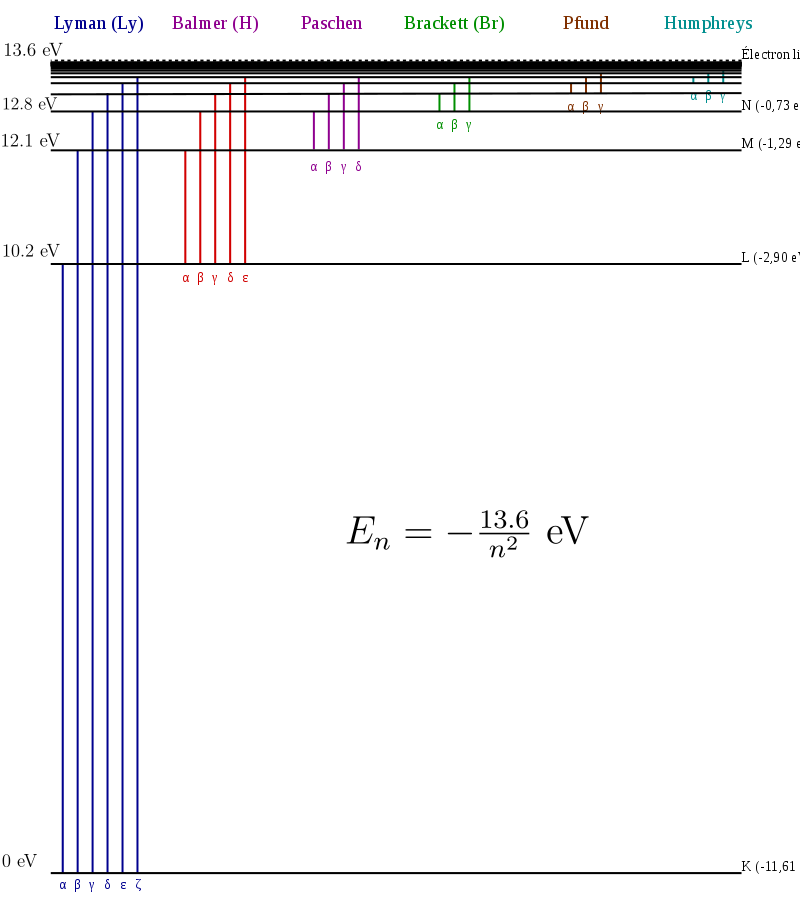
\includegraphics[width=0.5\textwidth]{figures/serie_idrogeno.png}
	\caption{\scriptsize Serie spettrale dell'idrogeno}
	\label{fig:-figures-serie_idrogeno-png}
\end{figure}
I livelli dell'atomo di idrogeno prendono la forma della Figura \ref{fig:-figures-serie_idrogeno-png}, possiamo notare diverse serie di energie che descrivono i livelli, ognuna avente il suo nome caratteristico.\\
Se mettiamo per comodità lo zero dell'energia sullo stato fondamentale abbiamo che i livelli energetici seguono la serie scritta in Figura \ref{fig:-figures-serie_idrogeno-png}.\\
Immaginiamo di voler far avvenire una transizione energetica dell'elettrone nell'idrogeno, a seconda del livello di partenza l'energia necessaria seguirà una determinata serie:
\begin{align}
	n=1 \ \to \ m \ge 2 \ &\implies \ \text{ Assorbimento da Lyman}\\
	n=2 \ \to m\ge 3 \ &\implies \ \text{ Assorbimento da Balmer} \\
			   &\ldots
.\end{align}
Il passaggio invece "dall'alto al basso" sarà l'emissione nelle varie serie.\\ 
Per la Lyman $\alpha $ ad esempio si ha che, se si emette o si assorbe un fotone dal primo stato eccitato al fondamentale (o viceversa) si ha che:
\begin{align}
	&\ce{n = 1 <-> n = 2 }  & E_{L_{\gamma \alpha }} = 10.2 \text{ eV}& &\lambda = 1216 \text{\AA}
.\end{align}
Mentre per la Lymann $\beta $:
\begin{align}
	&\ce{n = 1 <-> n = 3 }  & E_{L_{\gamma \beta  }} = 12.1 \text{ eV}& &\lambda = 1020 \text{\AA}
.\end{align}
E così via fino al salto di Lymann
\begin{align}
	&\ce{n = 1 <-> n = \infty }  & E_{L_{\infty}} = 13.6 \text{ eV}& &\lambda = 912 \text{\AA}
.\end{align}
Vediamo che questa serie è tutta nell'ultravioletto, questo è importante e dobbiamo tenerlo a mente.\\
Un'altra serie importante è la Balmer:
\begin{align}
	&\ce{n = 2 <-> n = 3 }  & E_{H_{\alpha }} = 1.9 \text{ eV}& &\lambda = 6563 \text{\AA}
.\end{align}
E così via fino al salto di Balmer:
\begin{align}
	&\ce{n = 2 <-> n = \infty }  & E_{H_{\infty }} = 3.5 \text{ eV}& &\lambda = 3646 \text{\AA}
.\end{align}
È utile notare che la serie di Balmer parte dal rosso e arriva all'ultravioletto con il salto, quindi gran parte della serie sta nel visibile, quindi quelle di Balmer sono le righe che possiamo vedere tecnicamente anche ad occhio nudo.
\subsection{Radiazione attraverso una nube interstellare}%
Ipotizziamo che il mezzo sia una nube di mezzo interstellare composta da idrogeno. La temperatura della nube è quella tipica di queste nubi: $T \approx 100$ K. Spariamo sulla nube due fasci aventi energie diverse:
\begin{align}
	&L_{\gamma,\alpha} \\
	&H_{\alpha}
.\end{align}
Ci chiediamo adesso se la nube sarà trasparente oppure opaca ai fasci inviati.\\
Se l'atomo di idrogeno si trova nello stato fondamentale allora il fotone dell'$H_{\alpha}$ non può essere assorbito, non ha l'energia per fare il salto, quindi tutti gli atomi di idrogeno sono invisibili per un fotone della $H_{\alpha}$. \\
Il fotone della $L_{\gamma,\alpha}$ invece ha l'esatta energia per effettuare il salto, quindi viene assorbito. \\
È quindi è importante capire se ci sono e quanti sono gli atomi nel primo eccitato, perchè se ci sono allora $H_{\alpha}$ viene assorbito avente l'esatta energia per permettere il salto. \\
Per capire se $H_{\alpha }$ viene assorito dalla nube è necessario capire in che stato si trovano gli atomi della nube.\\
Procediamo quindi assumendo che la nube sia all'equilibrio termodinamico e cerchiamo il rapporto tra gli atomi del primo eccitato e quello fondamentale con la distribuzione di Boltzmann:
\[
	\frac{n_2}{n_1} = \frac{g_2}{g_1}\exp\left( -\frac{\Delta E_{1,2}}{kT} \right) 
.\] 
Le $g$ sono le degenerazioni dell'atomo di idrogeno (i pesi statistici): $g_{n}= 2 n^2$ mentre $n_2$ è il numero di atomi di idrogeno che si trovano nel primo eccitato, $n_1$ è il numero di quelli che si trovano nel fondamentale. \\
Abbiamo che $ \ g_2 = 8 \ $, $ \ g_1 = 2 \ $,  $ \ \Delta E _{1,2}= 10.2 \ $eV, $ \ kT =\frac{1}{120} \ $ eV \footnote{Per ricordare questa si può ricordare che a temperatura ambiente kT = $\frac{1}{40}$ eV, quindi si ricava anche alla nostra temperatura. Sulla superficie del sole, con temperature dell'ordine di 6000 K, sarà circa mezzo eV (emissione nel visibile). Nel centro del sole invece, con circa 16 milioni di K, si ha $kT \approx$ 1 keV (emissione nell'X).}.\\
\[
	\frac{n_2}{n_1} = 4 \exp\left( - \frac{10.2}{1 / 120} \right)  = 4 \exp\left( -1224 \right) = 4\cdot 10^{-1224 /2.3} \approx 10^{-532}
.\] 
Dove abbiamo usato il fattore di conversione tra esponenziali nelle due basi.\\
Abbiamo un atomo nell'eccitato ogni $10^{532}$ atomi nel fondamentale. Bisonga capire quanti atomi ha la nube per dire se il numero di atomi che si trovano effettivamente nel primo eccitato non è trascurabile. \\
Per risolvere la questione basta però notare che $10^{532}$ sono troppi atomi persino per l'universo stesso!
\paragraph{Stima del numero di atomi nell'universo}%
La massa del sole è $2 \cdot 10^{33} $ g, la massa dell'idrogeno $M_{H} = 1.66 \cdot 10^{-24}$ g quindi il numero di atomi nel sole sarà dell'ordine di $n_{_{\odot}} = 10^{57}$, nella galassia ci sono circa $10^{11}$ stelle, quindi il numero di particelle idrogenoidi nella galassia potrebbe essere dell'ordine di $n_{\text{galassia}} \approx 10^{68}$. 
Visto che ci sono nell'universo visibile abbiamo circa $10^{11}$ galassie, quindi in tutto nell'universo visibile possiamo stimare circa $n_{\text{universo}} \approx 10^{80}$ atomi. 
Un numero incredibiblmente più piccolo di quello trovato da noi sopra.\\
Tornando all'esercizio possiamo stare molto tranquilli sul fatto che nella nube non ci saranno idrogeni nel primo eccitato, saranno tutti nel fondamentale, quindi la nube è otticamente sottile al fascio $H_{\alpha}$ anche se fosse estesa per milioni di chilometri.\\
Viceversa i fotoni della $L_{\alpha }$ verranno assorbiti, la nube sarà opaca a questi fotoni.\\
Questo ci anticipa anche che se in un mezzo come quello sopra gli atomi si eccitano (tipicamente per collisioni) e si diseccitano successivamente nella $H_{\alpha }$ allora i fotoni emessi usciranno dal mezzo indisturbati portando con se dell'energia. 
Questo è una tecnica di raffreddamento per il mezzo stesso che può perdere energia per collisioni e successiva emissione.\\
Inoltre se andiamo sul sito dell'hubble space telescope e cerchiamo le regioni di formazione stellare $H_2$ vediamo delle regioni di un colore rossastro, questo è proprio $H_{\alpha }$ che, con i suoi $6563$ \AA $ \ $  esce dalla nube per arrivare alla lente di Hubble.
\begin{figure}[H]
	\centering
	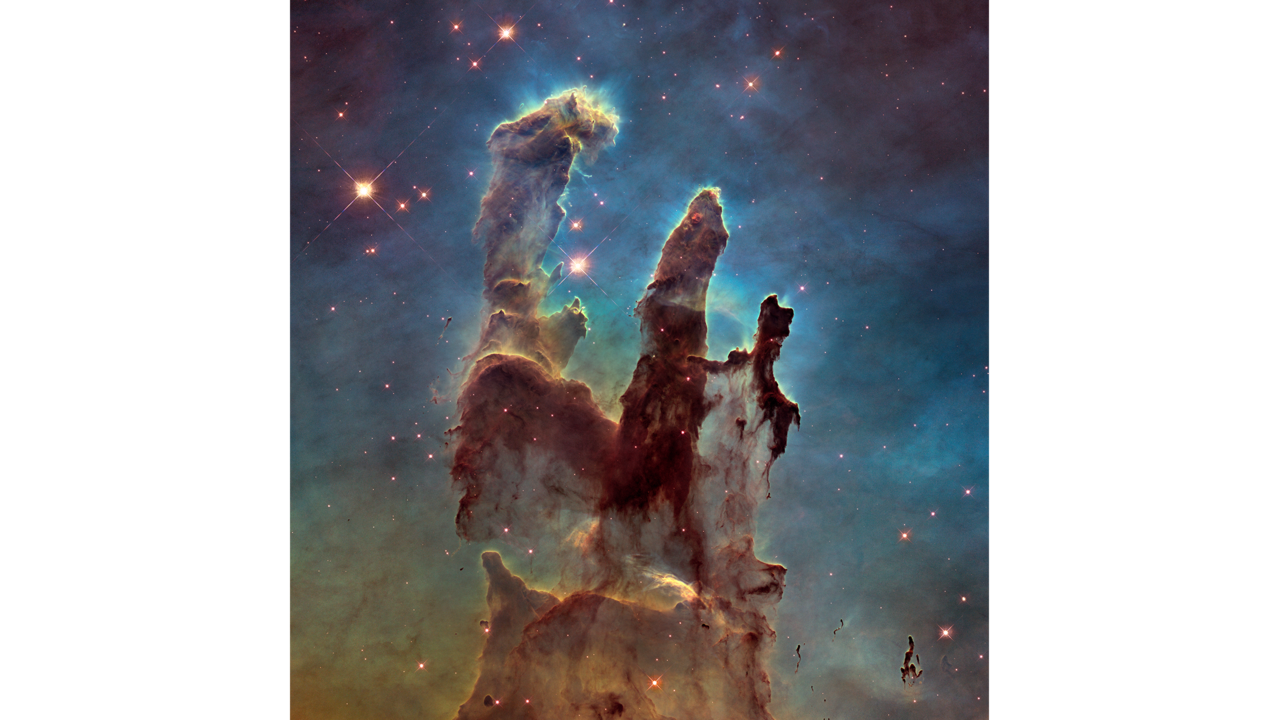
\includegraphics[width=0.8\textwidth]{figures/veil-nebula.png}
	\caption{\scriptsize Immagine di una nebulosa nel visibile (modificata per accentuare la nitidezza).}
	\label{fig:figures-veil-nebula-png}
\end{figure}
\noindent
\subsection{Soluzione analitica all'equazione del trasporto stazionaria.}%
Abbiamo visto che l'espressione dell'equazione del trasporto in condizioni stazionarie si riduce a:
\[
	\frac{\mbox{d} I_{\nu}}{\mbox{d} s} = j _{\nu} - \alpha_{\nu}I_{\nu} 
.\] 
Vogliamo fare un cambio di variabile, anzichè studiarla rispetto alla variabile $s$ la vogliamo rispetto alla profondità ottica $\tau _{\nu} $.
\[
	\frac{\mbox{d} I_{\nu}}{\mbox{d} s} = \frac{\mbox{d} I_{\nu}}{\mbox{d} \tau_{\nu}} \frac{\mbox{d} \tau_{\nu}}{\mbox{d} s} = \frac{\mbox{d} I_{\nu}}{\mbox{d} \tau_{\nu}} \alpha_{\nu} = j _{\nu} - \alpha_{\nu}I_{\nu}
.\]
L'equazione modificata diventa:
\[
	\frac{\mbox{d} I_{\nu}}{\mbox{d} \tau_{\nu}}  = \frac{j _{\nu}}{\alpha_{\nu}}- I_{\nu}
.\] 
Possiamo allora definire il primo termine dopo l'uguale come:
\begin{defn}[Funzione sorgente]{def:Funzione sorgente}
	Il rapporto tra il coefficiente di emissione ed il coefficiente di assorbimento è detto funzione sorgente $s_{\nu} $:
	\[
		s_{\nu} = \frac{j _{\nu} }{\alpha _{\nu} }
	.\] 
\end{defn}
L'equazione del trasporto con questo termine è ovviamente:
\[
	\frac{\mbox{d} I_{\nu}}{\mbox{d} \tau_{\nu}} = s_{\nu}- I_{\nu}
.\] 
Possiamo notare inoltre che 
\[
s_{\nu}<I_{\nu} \implies \frac{\mbox{d} I_{\nu}}{\mbox{d} \tau_{\nu}} <0
.\]
In questo modo l'intensità del fascio viene attenuata nell'attraversare la nube. Viceversa:
\[
s_{\nu}>I_{\nu} \implies \frac{\mbox{d} I_{\nu}}{\mbox{d} \tau_{\nu}} >0
.\]
Quindi il fascio viene amplificato nel passagio.\\
Proviamo a risolvere formalmente l'equazione:
\[
	\frac{\mbox{d} I_{\nu}}{\mbox{d} \tau_{\nu}}e^{\tau_{\nu}} = s_{\nu}e^{\tau_{\nu}}- I_{\nu}e^{\tau_{\nu}}
.\] 
Quindi possiamo raggruppare:
\[
	\frac{\mbox{d} }{\mbox{d} \tau _{\nu} } \left( I_{\nu}e^{\tau_{\nu}} \right) = s_{\nu}e^{\tau_{\nu}}
.\] 
e integriamo tra 0 e $\tau _{\nu} $:
\[
	\int_{0}^{\tau_{\nu}}\frac{\mbox{d} }{\mbox{d} \tau'_{\nu}} \left( I_{\tau'_{\nu} } e^{\tau' _{\nu} } \right) d\tau '_{\nu}  = 
	\int_{0}^{\tau _{\nu} } s( \tau '_{\nu} ) e^{\tau '_{\nu} }d\tau _{\nu} 
.\] 
integrando il primo termine ottiene: 
\[
	I_{\nu}\left( \tau_{\nu} \right) e^{\tau_{\nu}} - I_{\nu}\left( 0 \right) = 
	\int_{0}^{\tau_{\nu}} s_{\nu}\left( \tau_{\nu}' \right) e^{\tau_{\nu}'}d \tau_{\nu}'
.\] 
Se dividiamo tutto per $e^{\tau _{\nu} }$ abbiamo la legge per $I_{\nu} ( \tau _{\nu} ) $.
\begin{fact}[Soluzione formale all'equazione del trasporto]{fact:Soluzione formale all'equazione del trasporto}
	\[
	I_{\nu}\left( \tau_{\nu} \right) = I_{\nu}\left( 0 \right)e^{-\tau_{\nu}} - \int_{0}^{\tau_{\nu}} \delta_{\nu}\left( \tau_{\nu}' \right) e^{-(\tau_{\nu}-\tau_{\nu}')}d \tau_{\nu}'
.\] 
\end{fact}
Il primo termine è la luce della sorgente estinta esponenzialmente dal mezzo a causa dell'assorbimento. Il secondo termine contiene il significato fisico di due distinti effetti: l'effetto dell'emissione di fotoni del fascio nei vari punti del mezzo ($s_{\nu} $) e l'effetto dell'assorbimento incluso nel termine esponenziale.\\
Innfatti il termine $\tau _{\nu} -\tau '_{\nu} $ sta ad indicare l'assorbimento dei fotoni che sono stati emessi dal mezzo. \\
Anche se abbiamo la soluzione generale resta il fatto che $s_{\nu} $ è incognita, anche se conoscessimo l'espressione analitica di $s_{\nu} $ non saremo comunque in grado di calcolare l'integrale poichè non conosciamo le condizioni fisiche (pressione, temperatura \ldots) del mezzo \footnote{dalle quali ricordiamo dipendere $\tau _{\nu} $}.
\paragraph{Esempio: mezzo omogeneo.}%
Se il mezzo è omogeneo per tutta la sua estensione si mantengono costanti le sue proprietà fisiche. Di conseguenza avremo che $\alpha _{\nu} $ e $j _{\nu} $ saranno uguali ovunque e la funzione sorgente sarà anch'essa una costante:
\[
	I_{\nu}\left( \tau_{\nu} \right) = I_{\nu}\left( 0 \right) e^{-\tau_{\nu}} + s_{\nu} e^{-\tau_{\nu}}\int_0^{\tau_{\nu}} e^{\tau_{\nu}'}d \tau_{\nu}' =
	I_{\nu}\left( 0 \right) e^{-\tau_{\nu}} + s_{\nu}\left( 1-e^{-\tau_{\nu}} \right) \label{eq:soluzione-mezzo-omogeneo}
.\] 
Possiamo iniziare ad intuire il significato fisico della funzione sorgente:
se il nostro fascio attraversa un mezzo otticamente profondo ($\tau_{\nu}\rightarrow \infty$) allora abbiamo che $I_{\nu}\left( \tau_{\nu} \right) \rightarrow s_{\nu}$. Allora la funzione sorgente è la grandezza fisica a cui tende l'intensità della radiazione se questa attraversa una regione otticamente spessa. Quindi ciò che succede al fascio in questo caso è una totale sostituzione dei fotoni provenienti dalla sorgente con i fotoni emessi all'interno del mezzo come in Figura \ref{fig:soluzione-all-equazione-del-trasporto-per-mezzo-otticamente-spesso}
\begin{figure}[H]
    %This is a custom LaTeX template!
    \centering
    \incfig{soluzione-all-equazione-del-trasporto-per-mezzo-otticamente-spesso}
    \caption{\scriptsize Sostituzione dei fotoni in un mezzo otticamente spesso.}
    \label{fig:soluzione-all-equazione-del-trasporto-per-mezzo-otticamente-spesso}
\end{figure}
\noindent
Man mano che la radiazione si propaga i fotoni del fascio perderanno le caratteristiche della radiazione sorgente ed acquisteranno invece la firma del mezzo.\\
Notiamo che questo non è soltanto un processo astrofisico, questo avviene anche quando guardiamo delle montagne lontane che ci appaiono celestine come il cielo:
\begin{figure}[H]
	\centering
	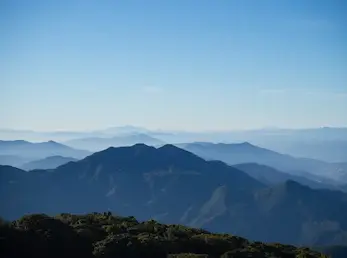
\includegraphics[width=0.4\textwidth]{figures/farmountain.png}
	\caption{\scriptsize Montagne lontane che acquistano il colore del cielo fino a dissolversi con esso.}
	\label{fig:figures-farmountain-jpg}
\end{figure}

\paragraph{Esempio: Mezzo omogeneo senza retroilluminazione}
In questo caso particolare abbiamo che $I_{\nu} ( 0) = 0$, l'unica radiazione che vediamo emergere è quella prodotta dal mezzo stesso.
\[
	I_{\nu} ( \tau _{\nu} ) = s_{\nu}\left( 1-e^{-\tau _{\nu} } \right)  
.\] 
Consideriamo adesso i casi in cui il mezzo è otticamene sottile o spesso alla radiazione che emerge da lui stesso.
\subparagraph{Mezzo otticamente sottile}
Siamo in questa situazione se $\tau _{\nu} \ll 1$, sviluppiamo l'esponenziale:
\[
	I_{\nu} ( \tau _{\nu} ) = s_{\nu} \tau _{\nu} 
.\] 
Visto che il mezzo è omogeneo si ha:
\[
	\tau _{\nu} = \int_{s_0}^{s} \alpha _{\nu} ( s') ds'= \alpha _{\nu} ( s-s_0)  = \alpha _{\nu} \cdot L
.\] 
Quindi abbiamo che:
\[
	I_{\nu} ( \tau _{\nu} ) = s_{\nu} \alpha _{\nu}\cdot  L = j _{\nu} \cdot L
.\] 
Dalla quale emerge l'importante contributo alla radiazione di $j _{\nu} $ in questa situazione.\\
Se il mezzo è costituito da atomi non completamente ionizzati allora sappiamo che la radiazione ha dei picchi in intensità molto marcati in corrispondenza della frequenza di transizione dei livelli, quindi sia il coefficiente di assorbimento $\alpha _{\nu} $ che il coefficiente di emissione $j _{\nu} $ avranno dei picchi molto marcati in corrispondenza di queste transizioni. Quindi qua ci aspettiamo proprio questo tipo di radiazione proveniente dal "mezzo", molto marcata in corrispondenza della transizione dei livelli delle specie atomiche. \\
Questa radiazione emergente sarà perciò caratterizzato da delle righe di emissione: uno spettro buio quasi ovunque con delle righe luminose.\\
Un esempio di questo tipo è un gas rarefatto riscaldato: una lampada al neon. Un esempio nello spazio sono le nebulose. \footnote{Nelle stelle invece vedo delle righe di assorbimento miste al continuo}
\subparagraph{Mezzo otticamente spesso}
Quando scaldiamo un oggetto a temperature elevate inizia ad essere percepibile la sua emissione di radiazione termica, questo passerà in modo continuo dal rosso scuro, poi al giallo, ecc\ldots \\
Prendiamo un mezzo omogeneo non retroilluminato ed otticamente spesso $\tau _{\nu} \gg 1$, in questo limite abbiamo che:
\[
	I_{\nu} ( \tau _{\nu} )  = s_{\nu} 
.\] 
Quindi la radiazione che emerge è uguale alla funzione sorgente, questo è il caso del oggetto riscaldato. Infatti la funzione sorgente è parente della radiazione di corpo nero che è una funzione della temperatura. Quindi in questo caso abbiamo uno spettro continuo.\\
Nel cosmo oggetti che approssimeranno questa radiazione sono le stelle, non sara esattamente una radiazione di corpo nero perchè abbiamo delle righe di assorbimento. Studieremo prossimamente da dove vengono queste misteriose righe di assorbimento.

%\lez{4}{02-03-2020}{}
\[
	\frac{\mbox{d} I_{\nu} }{\mbox{d} s} = j _{\nu} -\alpha _{\nu} \quad d\tau _{\nu} = \alpha _{\nu} ds \text{ Profondità ottica}
.\] 
\[
	\frac{\mbox{d} I_{\nu} }{\mbox{d} \tau _{\nu} } = s_{\nu} - I_{\nu} \quad S_{\nu} = \frac{j _{\nu} }{\alpha _{\nu} } \text{S: funzione sorgente}
.\] 
Soluzione formale eq. trasporto
\[
	I_{\nu} ( \tau _{\nu} ) = I_{\nu} ( 0) e^{-\tau _{\nu} } + \int_{0}^{\infty} s_{\nu} ( \tau _{\nu} ) e^{-\left( \tau _{\nu} -\tau _{\nu} ' \right) }
	\text{ messo omogeneo}
.\] 
Caso di mezzo omogeneo:
\[
	I_{\nu} ( \tau _{\nu} ) = I_{\nu} ( 0) e^{-\tau _{\nu} } + S_{\nu} \left( 1- e^{-\tau _{\nu} } \right) 
.\] 
\[
	\text{Se } \tau _{\nu} \gg 1 \implies I_{\nu} ( \tau _{\nu} ) \to S_{\nu} 
.\] 
Altrimenti
\[
	I_{\nu} ( \tau _{\nu} )  \approx j _{\nu} L
.\] 
\subsection{Scoperta delle righe}%
Le righe sono state scoperte osservando lo spettro del sole, 



%\lez{5}{09-03-2020}{}
\subsection{Atmosfera a piani paralleli.}%
In oggetti come le stelle è spesso comodo studiare la struttura "strato per strato", il modello di atmosfere a piani paralleli consiste nel considerare una atmosfera
\begin{itemize}
	\item divisa a strati paralleli l'uno tra l'altro
	\item ambienti privi di curvatura
\end{itemize}
\begin{figure}[H]
    %This is a custom LaTeX template!
    \centering
    \incfig{amtosfera-a-piani-paralleli}
    \caption{\scriptsize Amtosfera a piani paralleli}
    \label{fig:amtosfera-a-piani-paralleli}
\end{figure}
\noindent
Per poter fare tale approssimazione è necessario che se chiamiamo la distanza tra uno strato e l'altro $d$ ed il raggio della stella $R$:
\[
	d\ll R
.\] 
Il vantaggio di questo modello è dovuto all'invarianza sotto rotazioni attorno a $z$, questo ci permette di semplificare moltissimo la scrittura di $I_{\nu}( \bs{r}, t, \bs{k}) $. Infatti questo dipenderà soltanto da $z$ per le coordinate spaziali, per il vettore d'onda invece avremo soltanto la dipendenza da $\theta$:
\begin{figure}[H]
    %This is a custom LaTeX template!
    \centering
    \incfig{dipendenza-da-theta-per-l-intensit-specifica}
    \caption{\scriptsize Dipendenza da theta per l'intensità specifica}
\end{figure}
\noindent 
Notiamo che con questo modello anche le quantità come Pressione, Temperatura, Densità saranno soltanto funzione di $z$.\\
Di consequenza otterremo che $I_{\nu} = I_{\nu} ( z, \theta )$ \footnote{Assumendo implicitamente le condizioni stazionarie.}. Vedremo che sarà molto utile adottare la convenzione:
\[
	\cos\theta = \mu  
.\] 
Ipotizziamo che $s$ sia il versore relativo alla direzione di propagazione del fascio, possiamo scrivere l'equazione del trasporto come:
\[
	\frac{\mbox{d} I}{\mbox{d} s} = j_{\nu} - \alpha _{\nu} I_{\nu} 
.\] 
Tuttavia nel modello delle atmosfere a piani paralleli conviene studiare questa equazione per la propagazione lungo $z$ anzichè lungo $s$, cambiamo quindi variabile:
\[
	dz = ds\cos\theta 
.\] 
\[
	\mu \frac{\partial I_{\nu} }{\partial z} = j _{\nu} -\alpha _{\nu} I_{\nu} 
.\] 
Prendiamo adesso per convenzione il centro della stella nella direzione opposta a quella indicata dall'asse $z$ e ridefiniamo la profondità ottica assumendola crescente andando verso l'interno (quindi di verso opposto a $z$).
A questo scopo quindi definiamo $\tau _{\nu} $ come:
\[
	d\tau _{\nu} = -\alpha _{\nu} dz
.\] 
Riscriviamo allora l'equazione del trasporto come:
\[
	\mu \frac{\partial I_{\nu} }{\partial \tau _{\nu} } = -s_{\nu} + I_{\nu} 
.\] 
Visto che $s_{\nu} = j_{\nu} /\alpha _{\nu} $.\\
Il nostro obbiettivo è adesso quello di risolvere questa equazione del trasporto nella variabile $\mu $. Moltiplichiamo a destra e sinistra per $\exp\left( -\tau _{\nu} /\mu  \right) $ e portiamo a sinistra i termini contenenti $I_{\nu}$:
\[
	\left( \mu \frac{\partial I_{\nu} }{\partial \tau _{\nu} } - I_{\nu}  \right) e^{-\frac{\tau_{\nu}}{\mu }} = -s_{\nu} e^{-\frac{\tau _{\nu} }{\mu }}
.\] 
Notiamo che il termine a sinistra è proprio una derivata:
\[
	\mu \frac{\mbox{d} }{\mbox{d} \tau _{\nu} } \left( I_{\nu} e^{- \frac{\tau _{\nu} }{\mu } } \right) = -s_{\nu} e^{- \frac{\tau _{\nu} }{\mu }}
.\] 
Integriamo da una profondità ottica $\tau _{\nu, 0}$ di partenza fino a $\tau _{\nu} $ a destra e sinistra:
\[
	\int_{\tau _{\nu ,0}}^{\tau _{\nu} } \mu \frac{\mbox{d} }{\mbox{d} \tau' _{\nu} } \left( I_{\nu} e^{- \frac{\tau' _{\nu} }{\mu } } \right)d\tau '_{\nu} =
	-\int_{\tau _{\nu , 0}}^{\tau _{\nu} } s_{\nu} e^{-\frac{\tau' _{\nu} }{\mu }}d\tau _{\nu} ' 
.\] 
Quindi risolvendo il primo integrale:
\[
	\left.\mu I_{\nu} ( \tau _{\nu} ', \mu ) e^{-\frac{\tau _{\nu} '}{\mu }}\right|_{\tau _{\nu, 0}}^{\tau _{\nu} } =
	-\int_{\tau _{\nu , 0}}^{\tau _{\nu} } s_{\nu} e^{-\frac{\tau' _{\nu} }{\mu }}d\tau _{\nu} ' \label{eq:I-APP}
.\] 
Possiamo adesso ditinguere due distinte situazioni che decreteranno i diversi valori di $\tau_{\nu, 0}$: 
\begin{enumerate}
	\item Raggi entranti nell'atmosfera dall'esterno.
	\item Fasci uscenti dall'atmosfera dall'esterno.
\end{enumerate}
\paragraph{Raggi uscenti dall'atmosfera}
Partiamo dal primo caso, questo corrisponde a 
\[
	0< \theta <\frac{\pi}{2} \implies 0 < \mu < 1
.\] 
Quindi siamo in una condizione in cui si passa da una zona otticamente spessa (il centro della stella) ad una zona otticamente sottile, per questo nel caso corrente avremo $\tau _{\nu ,0}= \infty$. Questo semplifica molto la soluzione all'equazione del trasporto, infatti resta:
\[
	I_{\nu} ( \tau _{\nu} ,\mu ) = - \int_{\infty}^{\tau _{\nu} } \frac{s_{\nu} ( \tau _{\nu} ') }{\mu } e^{- \frac{\tau _{\nu} ' - \tau _{\nu} }{\mu }}d\tau _{\nu} '
.\] 
\paragraph{Raggi entranti.}
Per considerare i raggi entranti in atmosfera adottiamo la convenzione per cui $\tau _{\nu} = 0$ sul "bordo esterno" di quest'ultima, con la consapevolezza che non c'è effettivamente un bordo esterno.\\
Secondo la nostra notazione siamo nell'intevallo:
\[
	\frac{\pi}{2}< \theta < \pi \implies -1 < \mu < 0 
.\] 
Notiamo che se esternamente niente irraggia allora per i raggi entranti avremo che $I_{\nu} ( \tau _{\nu} = 0) = 0$, questo è il caso ad esempio di una stella solitaria.\\

Possiamo adesso fare l'assunzione di essere in una atmosfera in LTE, in questo modo pur non conoscendo il profilo di temperatura della stella $T( \tau _{\nu} ) $ siamo in grado di ricavare molte utili informazioni su quest'ultima.\\
Inanzitutto con l'equilibrio termodinamico locale abbiamo per la legge di Kirchhoff
\[
	s_{\nu} ( \tau _{\nu} ) = B_{\nu} ( \tau _{\nu} ) 
.\] 
Quindi possiamo cercare di ricavare $I_{\nu} ( \tau _{\nu}, \mu  ) $ risolvendo l'integrale della \ref{eq:I-APP} nelle varie situazioni.\\
All'interno di tale formula abbiamo un integrale della funzione $s( \tau _{\nu} ') $, con  $\tau _{\nu} '$ che può variare in un intervallo tale da farci venire dei dubbi sulla corretta applicabilità della LTE. Per correggere questo fatto possiamo considerare la correzione al primo ordine per $s( \tau _{\nu} ) $:
\[
	s( \tau _{\nu}' ) \approx B_{\nu} ( \tau _{\nu} ) + ( \tau _{\nu} ' - \tau _{\nu} ) \frac{\mbox{d} B_{\nu} }{\mbox{d} \tau _{\nu} } + \ldots
.\] 
Ipotizziamo quindi adesso che sia sufficiente la prima correzione e vediamo cosa succede nel caso di \texttt{Raggi uscenti}.
\begin{align}
	I_{\nu} ( \tau _{\nu} , \mu ) =&  \int_{\infty}^{\tau _{\nu} } \left[ B_{\nu} ( \tau _{\nu} ) + \left( \tau _{\nu} ' - \tau _{\nu}   \right) \frac{\mbox{d} B_{\nu} }{\mbox{d} \tau _{\nu} } \right] e^{-\frac{\tau _{\nu} ' -\tau _{\nu} }{\mu }} d\tau _{\nu} ' = \\
	= & B_{\nu} ( \tau _{\nu} ) \int_{\infty}^{\tau _{\nu} } e^{-\frac{\tau _{\nu} ' -\tau _{\nu} }{\mu }} \frac{d\tau _{\nu} '}{\mu } -
	\frac{\mbox{d} B_{\nu} }{\mbox{d} \tau _{\nu} } \int_{\infty}^{\tau _{\nu} }  \left( \tau _{\nu} ' - \tau _{\nu}  \right) e^{-\frac{\tau _{\nu} ' -\tau _{\nu} }{\mu }} \frac{d\tau _{\nu} '}{\mu }
.\end{align}
Risolvendo i due integrali si ottiene:
\[
	I_{\nu} ( \tau _{\nu} , \mu ) = B_{\nu} ( \tau _{\nu} ) + \mu \frac{\mbox{d} B_{\nu} }{\mbox{d} \tau _{\nu} } 
.\] 
Otteniamo così una brillanza che è frutto di due contributi: il primo che è quello di corpo nero a noi già noto, il secondo è una correzione anisotropa che dipende dalla direzione di propagazione.
Questo risultato ci dice che nel caso in cui vi è un gradiente di temperatura vi sarà anche una variazione di $B_{\nu} ( \tau _{\nu} ) $.
\[
	\frac{\mbox{d} B_{\nu} }{\mbox{d} \tau _{\nu} } \neq 0 \leftrightarrow \nabla T \neq 0
.\] 
Vediamo adesso se le grandezze introdotte (alcune delle quali erano momenti di vario ordine) sono utili alla soluzione della nostra atmosfera. Ricordiamo che:
\[
	u_{\nu} = \int \frac{I_{\nu} }{c}d\Omega  = \frac{2p}{c}\int_{-1}^{1} I_{\nu} d\mu  
.\] 
\[
	F_{\nu} = 2\pi \int_{-1}^{1} I_{\nu} \mu d\mu  
.\] 
\[
	P_{\nu} = \int \frac{I_{\nu} }{c}\cos^2\theta d\Omega = \frac{2\pi}{c}\int_{-1}^{1} I_{\nu} \mu ^2d\mu  
.\] 
\[
	J_{\nu} = \int \frac{I_{\nu} }{4\pi}d\Omega = \frac{1}{2}\int_{-1}^{1} I_{\nu} d\mu  \implies u_{\nu} = \frac{4\pi}{c}J_{\nu} 
.\] 
Cercheremo di sfruttare  queste quantità per trarne informazioni sul sistema. Partiamo dalla densità di energia:
\begin{align}
	u_{\nu} =& \frac{2\pi}{c}\int_{-1}^{1} I_{\nu} d_{\nu} =\\
	=& \frac{2\pi}{c}\int_{-1}^{1}B_{\nu} ( \tau _{\nu} )d\mu  + \int_{-1}^{1}\mu \frac{\mbox{d} B_{\nu} }{\mbox{d} \tau _{\nu} } d\mu =\\
	=& \frac{2\pi}{c}\left[ B_{\nu} ( \tau _{\nu} ) \int_{-1}^{1} d\mu + \frac{\mbox{d} B_{\nu} }{\mbox{d} \tau _{\nu} } \int_{-1}^{1} \mu d\mu   \right] =\\
	=& \frac{4\pi}{c}B_{\nu} ( \tau _{\nu} ) 
\end{align}
Si scopre così che la densità di energia rimane la stessa del caso di corpo nero nonostante la correzione.\\
Proviamo ad effettuare il conto anche per il flusso:
\[
	F_{\nu} = 2\pi \int_{-1}^{1} I_{\nu} \mu d\mu = \ldots = \frac{4\pi}{3}\frac{\mbox{d} B_{\nu} }{\mbox{d} \tau _{\nu} } 
.\] 
Si scopre quindi che il flusso non è nullo come nel caso di corpo nero, bensì l'anisotropia permette di avere un flusso uscente proporzionale alla variazione di $B_{\nu} $ assente nel caso isotropo.
\[
	F \neq 0 \leftrightarrow \nabla T \neq 0
.\]
Facendo il calcolo anche per $P_{\nu} $ si ottiene:
\[
	P_{\nu} = \frac{4\pi}{3c}B_{\nu} ( \tau _{\nu} ) 
.\] 
Coerente con la nota formula: $P_{\nu} = u_{\nu} /3$.
\subsection{Valutazione della anisotropia.}%
Possiamo valutare l'anisotropia della nostra sorgente nel seguente modo:
\[
	\frac{\frac{\mbox{d} B_{\nu} }{\mbox{d} \tau _{\nu} } }{B_{\nu} ( \tau _{\nu} ) } = \frac{\frac{3F_{\nu} }{4\pi}}{\frac{cu_{\nu} }{4\pi}}= \frac{3}{c}\frac{F_{\nu} }{u_{\nu} }
.\] 
Visto che vogliamo soltanto una stima qualitativa anzichè valutare le quantità monocromatiche valutiamo quelle integrate sulla frequenza:
\[
	\frac{\frac{\mbox{d} B_{\nu} }{\mbox{d} \tau _{\nu} } }{B_{\nu} ( \tau _{\nu} ) } \approx \frac{3F}{c u} = \frac{3}{c} \frac{\sigma T_{\text{eff}}^{4}}{aT^{4}} = \frac{3}{4}\left( \frac{T_{\text{eff}}}{T} \right) ^{4}
.\] 
Quindi se andando verso l'interno la temperatura $T$ aumenta mi aspetto che il contributo anisotropo sia sempre minore. Di conseguenza il nostro sviluppo di $s_{\nu} $ perde di significato se andiamo in strati atmosferici tali che $T_{\text{eff}} > T$.
\subsection{Atmosfera grigia}%
Anche se stiamo facendo passi avanti non abbiamo ancora trovato il profilo di temperatura, in genere questa è una operazione molto complicata, ci sono corsi appositi. \\
Il caso che affrontiamo noi è quello semplificato di Atmosfera Grigia:
\begin{defn}[Atmosfera grigia]{def:Atmosfera grigia}
	Ambiente avente $\alpha _{\nu} $ costante per ogni frequenza.
\end{defn}
In questo modo $\tau _{\nu} $ non dipende anch'esso dalla frequenza. Possiamo allora integrare tutte le quantità studiate nella frequenza senza problemi.\\
L'equazione del trasporto diventa:
\[
	\mu \frac{\mbox{d} I}{\mbox{d} \tau } = - s + I \label{eq:trasport-parallel-plane}
.\] 
Possiamo adesso trovare i momenti dell'equazione del trasporto. Moltiplichiamo a destra e sinistra per $\frac{1}{2}$ e integriamo in $\mu $ per l'ordine zero:
\[
	\frac{1}{2}\int_{-1}^{1} \mu \frac{\partial I}{\partial \tau } d\mu  = \frac{1}{2} \int_{-1}^{1} sd\mu + \frac{1}{2}\int_{-1}^{1} I d\mu  
.\] 
Portando fuori la derivata dal primo integrale, ricordando la definizione di $J$ e considerando che $s$ non dipende dall'angolo di emissione si ottiene:
\[
	\frac{1}{4\pi} \frac{\mbox{d} F}{\mbox{d} \tau }  = - s + J \label{eq:flux_0}
.\] 
Se ripetiamo l'operazione con il momento di ordine 1, moltiplicando ambo i membri per $\frac{2\pi}{c} \mu $ si ottiene:
\[
	\frac{\mbox{d} P}{\mbox{d} \tau } = \frac{F}{c}
.\] 
Anche questo è un risultato utile, infatti il flusso è non nullo soltanto se vi è una variazione della pressione radiativa.

%\lez{6}{12-03-2020}{}
Procediamo con il conto della scorsa lezione assumendo l'equilibrio radiativo nella nostra atmosfera, ovvero l'assenza di sorgenti e di pozzi in quest'ultima. In questo modo il flusso che arriva al nostro strato dalle profondità dell'atmosfera è conservato e passa oltre, quindi:
\[
	\frac{\partial F}{\partial \tau } = 0 
.\] 
In questo modo si ricava dalla \ref{eq:flux_0} che:
 \[
	J = s
.\] 
Quindi l'equazione del trasporto (\ref{eq:trasport-parallel-plane}) diventa:
\begin{align}
	\mu \frac{\mbox{d} I}{\mbox{d} \tau } =& - J + I =\\
	= & I - \frac{1}{2}\int_{-1}^{1} I( \tau )  d\mu  
.\end{align}
Quest'ultima è una equazione integro-differenziale in $I$, si risolve con dei metodi analitici particolari che vanno fuori dalla portata del corso.\\
Vediamo allora se studiandone i momenti possiamo far in modo di trovare una soluzione, seppur restringendo ancora il campo della soluzione. Partiamo dal momento di ordine 1:
\begin{align}
	&\frac{\mbox{d} P}{\mbox{d} \tau } = \frac{F}{c} &
	&\ce{ ->[Integro]}
	& P( \tau ) = \frac{F}{c}\left( \tau + q \right) 
.\end{align}
Dove $q$ è una costante di integrazione. Vedremo che trovare questa costante ci permetterà di risolvere l'atmosfera.\\ 
Abbiamo visto che in caso di LTE e considerando solo la prima correzione alla legge di Kirchhoff continua ad esser valido che:
\[
	P = \frac{u}{3}
.\] 
Questa abbiamo detto esser valida fintanto che il contributo anisotropo è piccolo rispetto a quello isotropo, quindi valido finchè non ci spostiamo verso strati esterni della atmosfera, tali che $T < T_{\text{eff}}$. Per proseguire con il conto analitico noi facciamo un'altra approssimazione:
\begin{defn}[Approssimazione di Eddington]{def:Approssimazione di Eddington}
	La relazione $P = u /3$ resta valida in tutta l'atmosfera, nonostante la possibile anisotropia.
\end{defn}
Possiamo quindi riassumere tutte le semplificazioni in cui ci siamo posti:
\begin{enumerate}
	\item Atmosfera a piani paralleli
	\item LTE (con correzione anisotropa)
	\item Atmosfera grigia
	\item Equilibrio radiativo
	\item Approssimazione di Eddington
\end{enumerate}
Grazie alla quinta è possibile inoltre affermare che resta vero in tutta l'atmosfera:
\[
	u = \frac{4\pi}{c}J
.\] 
E inoltre vale sempre che $J = s$.\\
Con questa nuova approssimazione possiamo mostrare la dipendenza di $s$ da $q$, infatti usando le ultime due relazioni si ha che:
\[
	P = \frac{4\pi J}{3c} = \frac{4\pi s}{3c} = \frac{F}{c}\left( \tau + q \right) 
.\] 
Quindi:
\[
	s( \tau )  = \frac{3F}{4\pi}\left( \tau + q \right) 
.\] 
Possiamo sfruttare questa espressione per la $s$ all'interno della soluzione che abbiamo trovato per $I_{\nu} $ nel caso di raggi uscenti dall'atmosfera ($0 \le \mu  \le 1$):
\[
	I( \tau , \mu )  = - \int_{\infty}^{\tau } \frac{s( \tau ') }{\mu } \exp\left(- \frac{\tau ' - \tau }{\mu } \right) d\tau ' 
.\]
Supponiamo di voler calcolare la brillanza nel punto più esterno alla nostra atmosfera, ovvero quello con $\tau = 0$, in tal caso avremo:
\[
	I( 0 , \mu )  = -  \int_{\infty}^{0 } \frac{s( \tau ') }{\mu } \exp\left(- \frac{\tau ' }{\mu } \right) d\tau ' 
.\] 
E sostituendo a questo punto la nostra $s$: 
\begin{align}
	I( 0, \mu ) =& - \int_{\infty}^{0} \frac{3F}{4\pi}\left( \tau ' + q \right) \exp\left( - \frac{\tau '}{\mu } \right)  d\tau '=\\
	=& - \frac{3F}{4\pi}
	\left[ \int_{\infty}^{0} \tau ' \exp\left( - \frac{\tau '}{\mu } \right) \frac{d\tau '}{\mu } + 
	q \int_{\infty}^{0} \exp\left( -\frac{\tau '}{\mu } \right) \frac{d\tau '}{\mu }  \right] =\\
	= &  \frac{3F}{4\pi}\left( \mu + q \right) 
.\end{align}
Un trucchetto che possiamo fare adesso è quello di trovare $F_{\text{out}}$ (uscente) in funzione di $I$, vedremo che facendo ciò il flusso si semplifichera permettendoci di ricavare $q$:
\begin{align}
	F_{\text{out}} =& 2\pi \int_{-1}^{1} I \mu d\mu = \\
	= & 2\pi \int_{-1}^{1} \frac{3F}{4\pi}\left( \mu + q \right) \mu d\mu = \frac{3F}{2}\left[ \int_{0}^{1} \mu ^2d\mu + \int_{0}^{1} \mu d\mu    \right] =\\
	= &\frac{3F_{\text{out}}}{2}\left[ \frac{1}{3} + \frac{q}{2} \right] 
.\end{align}
Quindi semplificando il flusso si ha:
\[
	q = \frac{2}{3}
.\] 
E inserendolo in $s( \tau ) $ e in $I_{\nu} ( 0, \mu ) $:
\[
	s( \tau ) = \frac{3F}{4\pi}\left( \tau + \frac{2}{3} \right) \quad \quad \quad I( 0, \mu ) = \frac{3F}{4\pi}\left( \mu + \frac{2}{3} \right) 
.\] 
Con queste informazioni possiamo per la prima volta trovare il profilo di temperatura per la nostra stella:
\[
	s = \frac{c}{4\pi} u = \frac{3F}{\pi}\left( \tau  + \frac{2}{3}\right) \implies cu = 3F\left( \tau + \frac{2}{3} \right) 
.\]
Ricordando che in LTE si ha anche $u = aT^{4}$, $F = \sigma  T^{4}$:
\[
	caT^{4}=3\sigma T_{\text{eff}}^{4}\left( \tau +\frac{2}{3} \right) \implies \left( T( \tau ) \right) ^{4}= \frac{3}{4}T^{4}_{\text{eff}}\left( \tau +\frac{2}{3} \right)  
.\] 
Notiamo nel nostro profilo che la temperatura efficace si ha per $\tau  = \frac{2}{3}$.\\
\subsection{Limb Darkening}%
Possiamo inoltre osservare un altro fenomeno interessante, infatti si ha che, all'aumentare dell'inclinazione $\mu $ diminuisce l'intensità uscente $I( 0, \mu ) $, questo da luogo al fatto che, per una sorgente che possiamo risolvere otticamente, la zona più interna risulterà più brillante della zona esterna.\\
Per convincerci del fatto che vi è un fenomeno del genere possiamo ragionare in termini di cammino libero medio $\tau $:
\begin{figure}[H]
    %This is a custom LaTeX template!
    \centering
    \incfig{fenomeno-di-limb-darkening}
    \caption{\scriptsize Fenomeno di Limb Darkening}
    \label{fig:fenomeno-di-limb-darkening}
\end{figure}
\noindent
Abbiamo visto che i fotoni che riescono ad emergere hanno cammino libero medio unitario, quindi hanno anche $\tau = 1$. \\
Ponendo un osservatore a sinistra in Figura \ref{fig:fenomeno-di-limb-darkening} possiamo notare che, andando verso l'esterno del disco la condizione $\tau =1$ è rispettata in zone sempre più superficiali. Se abbiamo che vale (quasi) la fisica del corpo nero per la stella e se la temperatura aumenta verso l'interno questo significa che raggi più profondi hanno anche intensità maggiore, quindi il centro del disco sarà più luminoso. Ecco spiegato il fenomeno del Limb Darkening in modo intuitivo.\\
Possiamo vedere questo effetto nel sole:
\begin{figure}[H]
	\centering
	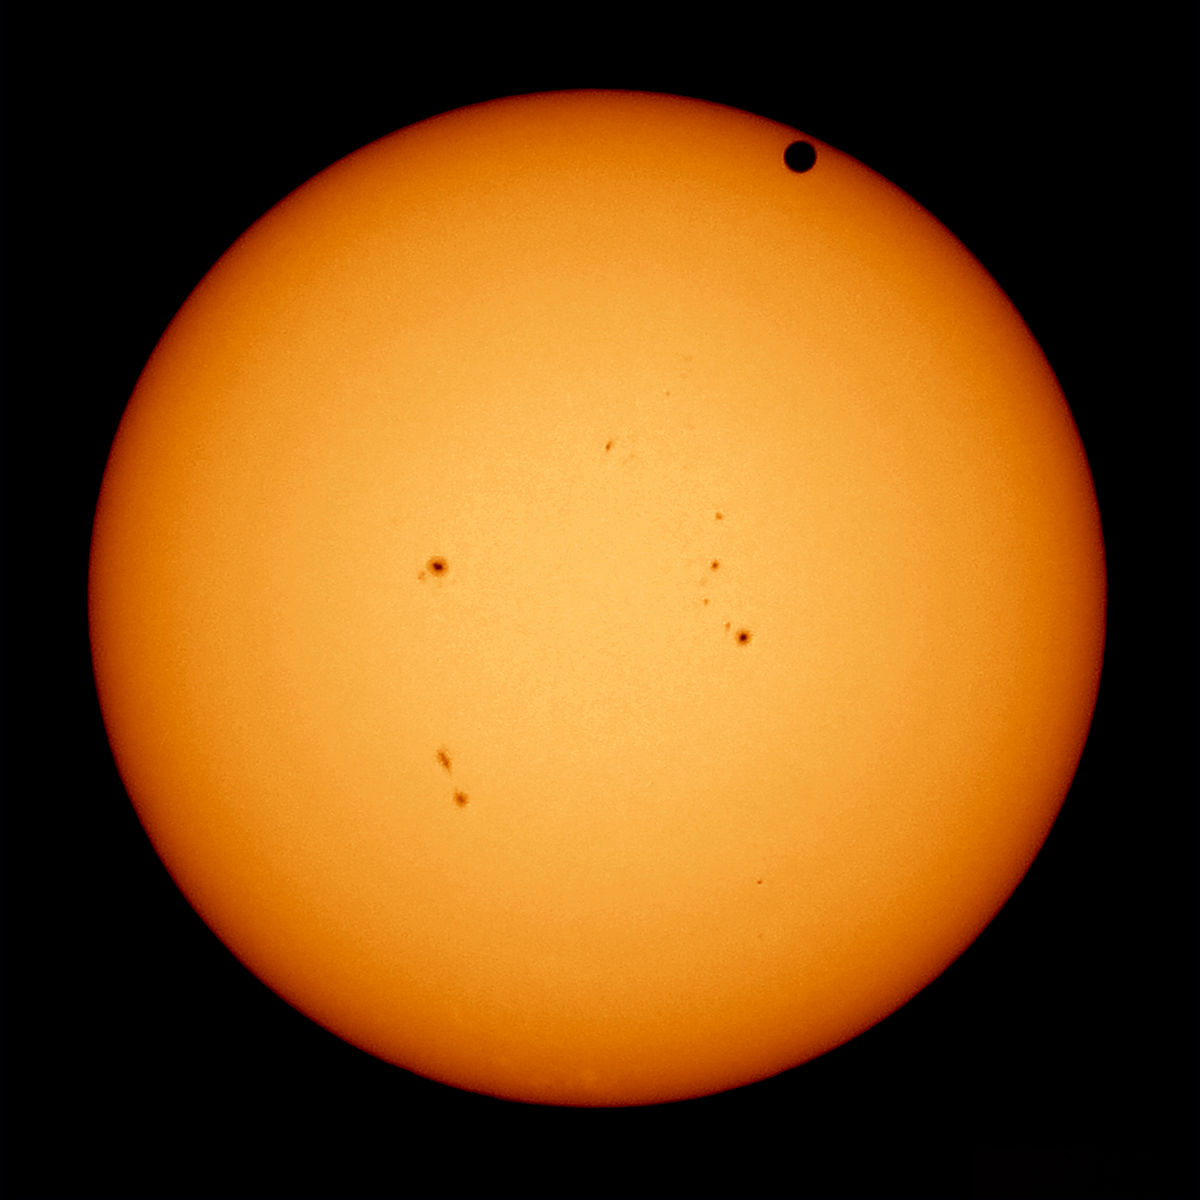
\includegraphics[width=0.6\textwidth]{figures/Limb.jpg}
	\caption{Limb Darkening nel disco del sole.}
	\label{fig:figures-Limb-jpg}
\end{figure}
\noindent
In cui con le stesse motivazioni (corpo nero ) si può spiegare anche l'effetto cromatico che, andando verso l'esterno si passa da giallo a rosso.\\
Concludiamo valutando l'intensità al centro su quella al bordo:
\[
	\frac{I( 0,0) }{I( 0,1) } = \frac{2F / 4\pi}{5F / 4\pi} = \frac{2}{5} 
.\] 
A conferma di quanto detto finora.
\subsection{Righe nello spettro stellare}%
Possiamo adesso spiegare  perchè nello spettro solare si possono trovare delle righe di assorbimento osservando dalla terra, abbandoniamo il modello di atmosfera grigia e torniamo a considerare le frequenze:
\[
	\mu \frac{\mbox{d} I_{\nu} }{\mbox{d} \tau _{\nu} } = -s_{\nu} + I_{\nu} 
.\]
I momenti della equazione sono gli stessi di prima, soltanto che adesso son monocromatici. Manteniamo l'ipotesi di equilibrio radiativo $F = cost$, considerando però il fatto che questo non significa che il flusso monocromatico $F_{\nu} $ sia costante, solo che il totale è conservato.
Quindi abbiam oche il flusso totale resta costante ma sarà ridistribuito tra le varie frequenze. \\
La radiazione che emerge dalla superficie può essere (qualitativamente) corretta con il primo ordine:
\[
	I_{\nu} ( 0, \mu ) \approx B_{\nu} ( 0) + \mu \frac{\mbox{d} B_{\nu} }{\mbox{d} \tau _{\nu} } 
.\] 
Concentriamoci sulla radiazione proveniente dal centro del disco $\mu = 1$:
\[
	I_{\nu} ( 0, 1) \approx B_{\nu} ( 0) +\frac{\mbox{d} B_{\nu} }{\mbox{d} \tau _{\nu} } \approx B_{\nu} ( \tau _{\nu} = 1) 
.\] 
Abbiamo ottenuto un risultato congruo con quanto visto sopra per il Darkening: dal centro del disco ci arrivano principalmente fotoni che si sono formati a  $\tau _{\nu} = 1$, infatti ci arriva una radiazione di corpo nero corrispondente a $B_{\nu} ( \tau _{\nu} = 1) $.\\
Prendiamo adesso un coefficiente di assorbimento fatto in questo modo: 
\begin{figure}[H]
    %This is a custom LaTeX template!
    \centering
    \incfig{coefficiente-di-assorbimento-per-una-riga}
    \caption{\scriptsize Coefficiente di assorbimento per una riga}
    \label{fig:coefficiente-di-assorbimento-per-una-riga}
\end{figure}
\noindent
Con questo coefficiente di assorbimento ci aspettiamo una riga, infatti abbiamo visto che il coefficiente di assorbimento ha le dimensioni di un inverso di un a lunghezza, abbiamo anche visto che questo decreta il cammino libero medio dei fotoni a tale frequenza $l_{\nu} $:
\[
	\alpha _{0} > \alpha _{c}
.\] 
\[
	l_{0} = \frac{1}{\alpha _{0}} < l_{c} = \frac{1}{\alpha _{c}}
.\] 
Quindi il cammino libero medio nell'intevallo di frequenze della riga sarà minore di quello nel continuo, questo spiega il motivo della presenza di righe di assorbimento. Infatti nella atmosfera stellare abbiamo visto essere presente un gradiente di temperatura (la temperatura aumenta andando verso l'interno), i fotoni che formano il continuo provengono da zone più profonde della atmosfera (in cui la temperatura è $T_{c}$), quelli della riga da zone più superficiali (in cui vi è $T_{0}$).
\[
	T_{0} < T_{c}
.\] 
Quindi se è vero che l'intensità proveniente dalla stella segue un andamento tipico di un corpo nero alla profondita ottica $\tau_{\nu} = 1$ ed è anche vero che le curve $B( \tau _{\nu} ) $ non si intersecano mai: 
\[
	I_{0} \approx B_{0}( T_{0}) <  I_{c} \approx B_{c}( T_{c}) 
.\] 
\begin{figure}[H]
    %This is a custom LaTeX template!
    \centering
    \incfig{riga-di-assorbimento}
    \caption{\scriptsize Riga di assorbimento}
    \label{fig:riga-di-assorbimento}
\end{figure}
\noindent
Quindi vediamo una intensità minore per le frequenze in cui $\alpha _{\nu} $ è "alto", viceversa sono più intense le frequenze per cui $\alpha _{\nu} $ è basso. Per questo motivo vediamo delle righe di assorbimento.

%\lez{7}{16-03-2020}{}
\subsection{Studio delle righe di assorbimento}
\label{subsec:Studio delle righe di assorbimento}
\subsubsection{Informazioni che ci arrivano dalle righe.}
\label{subsubsec:Informazioni che ci arrivano dalle righe.}
L'identificazione delle righe negli spettri stellari è molto importante, infatti dalla conoscenza della lunghezza d'onda centrale della riga possiamo conoscere:
\begin{itemize}
	\item L'atomo che le ha causate assorbendo fotoni.
	\item Lo stato energetico dell'atomo (perchè una data lunghezza d'onda corrisponde ad una determinata transizione energetica).
	\item Lo stato di ionizzazione dell'atomo: atomi dello stesso elemento chimico ma in stati di ionizzazione differenti hanno livelli energetici differenti e quindi tranzizioni differenti.
	\item La temperatura dell'atmosfera di quell'elemento: il popolamento dei livelli energetici associati alla transizione incriminata dipenderà dalla temperatura.
	\item La densità di quell'elemento nella atmosfera.
\end{itemize}
Naturalmente le ultime due informazioni citate, che riguardano la condizione fisica della atmosfera in cui l'atomo è immerso, riguardano esclusivamente la fotosfera della stella se facciamo osservazione nel visibile.\\
Un'altro parametro che può darci molte informazioni è la larghezza della riga, vediamo un esempio di riga nello spettro per avere un pò di nomenclatura di riferimento:
\begin{figure}[H]
    \centering
    \incfig{riga-di-assorbimento-generica-nello-spettro}
    \caption{Riga di assorbimento generica nello spettro.}
    \label{fig:riga-di-assorbimento-generica-nello-spettro}
\end{figure}
\noindent
\subsubsection{Allargamento di una riga.}
\label{subsubsec:Allargamento di una riga.}
Dobbiamo trovare un indicatore che misuri l'intensità della riga rispetto al continuo adiacente. La quantità di energia che viene sottratta al continuo in questo caso è l'area della conca in Figura \ref{fig:riga-di-assorbimento-generica-nello-spettro}. Questa area è chiamata area equivalente:
\begin{defn}[Area equivalente di una riga $A( \lambda ) $]{def:Area equivalente di una riga}
	Data una riga come in Figura \ref{fig:riga-di-assorbimento-generica-nello-spettro} l'area equivalente della riga è definita come:
\[
	A( \lambda_0) = \int_{\lambda_1}^{\lambda_2} \left( I_{c}-I_{\lambda} \right) d\lambda  
.\]
\end{defn}
Questo parametro è molto importante, infatti decide se saremo in grado di studiare tale riga oppure no: se la riga è troppo sottile può succedere che non si possa risolvere con lo strumento utilizzato per la misura, analogamente se abbiamo righe troppo larghe potremmo non essere in grado di distinguerle dal continuo.\\
Possiamo allora mettere in evidenza quest'ultima affermazione definendo il parametro di larghezza equivalente come:
\begin{defn}[Larghezza equivalente $W( \lambda ) $]{def:Larghezza equivalente}
	La larghezza equivalente è l'Area equivalente normalizzata sull'intensità del continuo:
	\[
	W( \lambda_0) = \frac{A( \lambda_0) }{I_{c}}= 
	\int_{\lambda_1}^{\lambda_2} \left( 1 - \frac{I_{\lambda} }{I_{c}}\right)d\lambda 
.\] 
\end{defn}
\subsubsection{Spessore minimmo di una riga}
\label{subsubsec:Spessore minimmo di una riga}
Il minimo spessore che una riga può avere è quella naturale, quella dovuta al decadimento spontaneo.\\
Prendiamo un atomo a due livelli, la probabilità che l'atomo si disecciti dal secondo livello al primo spontaneamente è proporzionale al coefficiente di Einstein A$_{2,1}$. Quindi la vita media sarà:
\[
	\Delta t = \frac{1}{A_{2,1}} 
.\] 
Ma dal principio di indeterminazione sappiamo che:
\[
	\Delta E\Delta t \ge \hbar
.\] 
Essendo $\Delta t$ finito ci dobbiamo aspettare un allargamento della riga che possiamo quantificare come:
\[
	\Delta \nu = \frac{\gamma _{\text{rad}}}{2\pi}
.\] 
con $\gamma _{\text{rad}}= 1 /\Delta t$, è chiamato Radiative Dumping Costant (RCT).\\
Nello specifico abbiamo che il profilo della emissione spontanea è dato da una Lorentziana:
\[
	\phi ( \mu ) = \frac{\gamma _{\text{rad}}}{2\pi}\frac{1}{\left( \mu -\mu_0 \right) ^2 + \left( \frac{\gamma _{\text{rad}}}{4\pi} \right) ^2}
.\] 
Per atomi con più livelli di eccitazione il parametro RCT si generalizza nel seguente modo:
\[
	\gamma _{\text{rad}} = \sum_{l}^{\infty} A_{kl} \quad k > l
.\] 
Le larghezze naturale delle righe tipicamente è dell'ordine di del millesimo dell' \AA. Tuttavia quando si guarda uno spettro la larghezza che otteniamo è in genere molto maggiore, di fatto la larghezza naturale è trascurabile.\\
Il motivo è che nelle atmosfere delle stelle ci sono altri processi di allargamento della riga aventi un contributo decisamente più importante dell'allargamento naturale.
\subsection{Processi di allargamento delle righe}
\label{subsubsec:Processi di allargamento delle righe}
I principali processi di allargamento dello spettro delle righe sono:
\begin{itemize}
	\item Allargamento termico.
	\item Allargamento collisionale (detto allargamento per pressione), questo cresce con l'aumento della densità dell'atmosfera.
	\item Allargamento per via di campi elettrici o magnetici.
	\item Allargamento rotazionale, questo per via del fatto che non risolviamo la stella e vi è comunque un effetto Doppler. 
\end{itemize}
\subsubsection{Allargamento termico.}
\label{subsubsec:Allargamento termico.}
Concentriamoci solo sulla velocità radiale degli atomi $v_r$: quella che sta sulla linea  della direzione di vista. La distribuzione di questa all'equilibrio termodinamico locale sarà:
\[
	dn( v_{r}) = n\sqrt{\frac{m}{2\pi kT}} 
	\exp\left( -\frac{m v_{r}^2}{2kT} \right) dv_r
.\] 
con $n$ è il numero di atomi per unità di volume dell'elemento interessato, $m$ la sua massa. Applichiamo adesso l'effetto Doppler alla frequenza:
\[
	\nu = \nu_0\left( 1 + \frac{v_r}{c} \right) 
.\] 
Abbiamo adottato la formula non relativistica dell'effetto Doppler, questo perchè alle temperature stellari gli atomi non si muovono abbastanza veloce da esser considerati relativistici. 
Facciamo un esempio: per l'idrogeno a $10000$ K la velocità termica abbiamo:
\[
	v_{\text{th}}
	=
	\sqrt{\frac{2kT}{m}} 
	\sim  \sqrt{\frac{ 2 \text{ eV}}{1 \text{ GeV/}c^2}} 
	\sim \sqrt{20}\cdot 10^{-4}c 
	\sim  13 \text{km}/\text{s}
.\] 
Osserviamo che per come abbiamo scritto la legge dell'effetto Doppler si ha un blue shift quando $v_r > 0$. Lo shift sarà dato da:
\[
	\Delta \nu 
	=
	\nu_0 \frac{v_r}{c}
.\] 
Utilizziamo quest'ultima per ricavarci la distribuzione in frequenza. Procediamo con il cambio di variabile:
\[
	v_r = \frac{c}{\nu_0}\left( \nu - \nu_0  \right) 
	\implies
	dv_r = \frac{c}{\nu_0}d\nu 
.\] 
Sostituendo quindi per la distribuzione in frequenza:
\[
	dn(\nu ) = n \sqrt{\frac{m}{2\pi kT}} \exp\left( - \frac{mc^2}{2\nu_0^2kT}\left( \nu -\nu_0 \right) ^2 \right) \frac{c}{\nu_0}d\nu 
.\] 
Quindi il profilo di riga diventerà, a causa della agitazione termica:
\[
	\phi ( \nu ) = \frac{1}{\Delta \nu_D\sqrt{\pi} }\exp\left( -\frac{\left( \nu -\nu_0 \right) ^2}{\Delta \nu_D^2} \right) 
.\] 
Con 
\[
	\Delta \nu_D = \frac{\nu_0}{c}\sqrt{\frac{2kT}{m}} 
.\] 
Questo è un profilo di tipo Gaussiano con $\Delta \nu _D$ che è detto allargamento Doppler. Questa larghezza cresce al crescere di $T$ e decresce al crescere di $m$.\\
A causa dei moti convettivi abbiamo anche un allargamento di riga per turbolenza, anche questo tipo di allargamento avrà un profilo Gaussiano, soltanto che non sarà dipendente dalla temperatura bensì dalla velocità di turbolenza.\\
Per tenerne di conto si definisce la seguente quantità 
\[
	\Delta \nu_D = \frac{\nu_0}{c}\sqrt{\frac{2kT}{m} + v_\text{turb.}^2} 
.\] 
Il profilo della riga viene spesso espresso in termini di lunghezza d'oonda, possiamo farlo effettuando il canbio di variabile, basta notare che:
\[
	\frac{\lambda - \lambda_0}{\lambda_0} \approx - \frac{\nu - \nu_0}{\nu_0}
.\] 
allora si ottiene facilmente che:
\[
	\phi 
	=
	\sqrt{\frac{mc^2}{2\pi kT\lambda_0^2}} 
	\exp\left( - 
	\frac{mc^2\left( \lambda -\lambda_0 \right)s^2 }{2kT \lambda_0^2} 
	\right) 
.\] 
Possiamo definire anche le quantità più importanti di questo profilo:
\[
	\sigma_\lambda  = \sqrt{\frac{kT}{mc^2}} \lambda_0
.\] 
\[
	FWHM = \sqrt{\frac{8kT \ln 2}{mc^2}} \lambda_0 
.\] 
\subsubsection{Allargamento per collisioni.}
\label{subsubsec:Allargamento per collisioni.}
In questo caso l'allargamento dipende dalla frequenza con cui avvengono le collisioni:
\[
	\nu _{\text{coll}} = n \sigma _{\text{coll}} v_{\text{coll}}
.\] 
Il profilo che si ottiene dalle collisioni è di tipo Lorentziano (come per l'emissione spontanea), si introduce quindi una una larghezza effettiva $\Gamma = \gamma _{\text{rad}} + 2 \nu _{\text{coll}}$, quindi:
\[
	\phi ( \nu ) = \frac{\Gamma }{4\pi^2}\frac{1}{\left( \nu -\nu_0 \right) + \left( \frac{\Gamma }{4\pi} \right) ^2}
.\] 
Nelle atmosfere stellari sono presenti tutti gli effetti citati sopra. Comunamente la zona centrale è dominata dall'allargamento Doppler, nelle code prevale l'effetto della Lorentziana.\\
Ci dobbiamo aspettare che nelle atmosfere rarefatte l'allargamento collisionale sia piccolo, e viceversa nelle atmosfere dense sarà importante. In questo modo si distinguono le stelle giganti da quelle nane.
\subsection{Magnitudine}%
La magnitudine è una misura della luminosità apparente di una stella, nata da Ipparco nel 2$^o$ secolo AC. La catalogazione di Ipparco in 6 classi di magnitudine è ancora usata oggi, con l'aggiunta di un pò di matematica moderna.\\
Le caratteristiche della catalogazione di Ipparco erano:
\begin{enumerate}
	\item Ordine decrescente di luminosità.
	\item Variazione di luminosità costante tra le 6 classi di luminosità.
\end{enumerate}
A rendere matematica questa classificazione è stato Pogston, egli utilizzò le seguenti considerazioni:
\begin{itemize}
	\item La sensibilita dell occhio è logaritmica
	\item Le stelle appartenenti alla sesta classe sono 100 volte meno luminose di quelle di classe uno.
\end{itemize}
Supponiamo di avere due stelle di luminosità apparenti $l_1$ e $l_2$, siano $m_1$ e $m_2$ le magnitudini apparenti di tali stelle. Per quanto assunto sopra avremo che:
\[
	\frac{l_1}{l_2}
	=
	\left( \frac{1}{100} \right) ^{\left( m_1-m_2 \right)/5}
	=
	10^{-2 /5 \left( m_1-m_2 \right) }
.\] 
Passando ai logaritmi:
\[
	\log \left( \frac{l_1}{l_2} \right) 
	=
	-\frac{2}{5}\left( m_1-m_2 \right) 
.\] 
La definizione moderna di magnitudine è quindi la seguente:
\begin{defn}[Magnitudine]{def:Magnitudine}
	Si definisce mangitudine $m_1$ di una stella relativa alla magnitudine di un'altra stella di riferimento $m_2$:
	\[
	m_1-m_2 = -2.5 \log \frac{l_1}{l_2}
	.\] 
	Dove $l_1$ e $l_2$ sono le luminosità apparenti relative alle due stelle.
\end{defn}

\subsubsection{Stelle di riferimento: misure relative di intensità}
Il modo utile di utilizzare la magnitudine è quello di scegliere una stella come riferimento con magnitudine $m_0$ per poter catalogare in maniera relativa tutte le altre stelle.\\
Se vogliamo ad esempio osservare la magnitudine della stella $m_*$ allora abbiamo:
\[
	m_{*}- m_0 = -2.5 \log \left( \frac{l_{*}}{l_0} \right) 
.\] 
Molti sistemi fotometrici usano come riferimento Vega, tra i quali anche il telescopio spaziale Hubble \footnote{Che usa come supporto anche uno spettro articificiale settabile a piacimento.}. Andiamo nel dettaglio sui sistemi di osservazione.
\subsubsection{Parametri di correzione per sistemi fotometrici.}
\label{subsubsec:Parametri di correzione per sistemi fotometrici.}
I limiti di osservazione di un sistema fotometrico sono:
\begin{enumerate}
	\item Non è mai possibile osservare l'intero spettro di emissione della sorgente.
	\item La sensibilità dello strumento nell'intervallo di frequenze che è possibile misurare non è costante.
\end{enumerate}
Per ovviare al fatto che non siamo in grado di conoscere il flusso di energia per unità di tempo e superficie $f( \lambda ) $ possiamo introdurre dei parametri di correzione che tengono di conto dei limiti della strumentazione e delle modifiche che il mezzo apporta alla sorgente.\\
Immaginiamo di poter osservare in un range di lunghezze d'onda da $\lambda_1$ a $\lambda_2$, immaginiamo inoltre che $f( \lambda ) $ sia il flusso della sorgente prima di entrare in atmosfera, la luminosità che si riesce ad osservare sarà data da:
\[
	l = \int_{\lambda_1}^{\lambda_2} f( \lambda ) T(\lambda) d\lambda   
.\] 
Il termine correttivo $T( \lambda ) $ tiene di conto di diversi effetti:
\[
	T( \lambda ) = R( \lambda ) K( \lambda ) Q( \lambda ) A( \lambda ) 
.\] 
Andiamo a vedere qual'è il ruolo di ciascuno di questi:
\begin{enumerate}
	\item $R( \lambda ) $: Riflettività. Questa è legata alle ottiche dello strumento.
	\item $K( \lambda ) $: Correzione alla risposta cromatica del filtro.
	\item $Q( \lambda ) $: Efficienza quantica del rilevatore. 
		Il rilevatore ha una risposta che dipende da $\lambda $.
	\item $A( \lambda ) $: Correzione sulla trasmissione in atmosfera terrestre.
\end{enumerate}
In conclusione possiamo riscrivere la magnitudine tenendo di conto della forma di $l$:
\[
	m_{*} 
	=
	- 2.5 \log \left( 
	\frac{
	\int_{\lambda_1}^{\lambda_2} 
	f_{*}( \lambda ) T( \lambda ) d\lambda }
	{
	\int_{\lambda_1}^{\lambda_2}  
	f_0( \lambda ) T( \lambda ) d\lambda } 
	\right) +
	m_0
.\] 
È quindi chiaro che per parlare di magnitudine è necessario esplicitare il nome dei parametri fissi che si scelgono per l'osservazione: il filtro utilizzato e la stella di riferimento.\\
Ipotiziamo di osservare una sorgente con due filtri differenti, si otterranno due magnitudini dello stesso oggetto differenti:
\[
	m_{*,i} 
	=
	- 2.5 \log \left( 
	\frac{
	\int_{\lambda_1}^{\lambda_2} 
	f_{*}( \lambda ) K_i( \lambda ) d\lambda }
	{
	\int_{\lambda_1}^{\lambda_2}  
	f_0( \lambda ) K_i( \lambda ) d\lambda } 
	\right) +
	m_{0,i}
.\] 
\[
	m_{*,j} 
	=
	- 2.5 \log \left( 
	\frac{
	\int_{\lambda_1}^{\lambda_2} 
	f_{*}( \lambda ) K_j( \lambda ) d\lambda }
	{
	\int_{\lambda_1}^{\lambda_2}  
	f_0( \lambda ) K_j( \lambda ) d\lambda } 
	\right) +
	m_{0,j}
.\]
Possiamo deinire la differenza di magnitudini apparenti come:
\begin{defn}[Indice di colore]{def:Indice di colore}
	L'indice di colore è la differenza di magnitudine apparente misurata con due filtri diversi.
	\[
		I = m_{*,i} - m_{*,j}
	.\] 
\end{defn}
Questo indice ci da una indicazione della temperatura della stella, infatti facendo la differenza tra le magnitudini in questione otteniamo il logaritmo del rapporto tra i flussi in due bande differenti. 
Proprio per questo tale indice ci da una indicazione della temperatura effettiva. \\
Abbiamo visto che possiamo approssimare lo spettro di una stella come quello di corpo nero, misurare lo spettro con due diversi filtri significa esplorare varie zone dello spettro:
\begin{figure}[H]
    \centering
    \incfig{significato-dell-indice-di-colore}
    \caption{Significato dell indice di colore}
    \label{fig:significato-dell-indice-di-colore}
\end{figure}
\noindent
Il rapporto tra le due aree colorate è proprio l'indice di colore. Vediamo dal grafico che tale indice può essere usato anche per una calibrazione dello strumento nella temperaura della stella osservata, infatti è evitende che il rapporto tra le aree vari al variare della temperatura grazie alla legge di spostamento di Wien.\\
\subsubsection{Magnitudine Bolemica.}
\label{subsubsec:Magnitudine Bolometrica.}
Si definisce magnitudine bolometrica la magnitudine in cui si raccoglie l'intero flusso proveniente dalla stella. Per ottenerla è necessario misurare la magnitudine in varie bande e mettere insieme i risultati.\\
La relazione che lega la magnitudine bolometrica a quella in una certa banda è la seguente:
\[
	m_{\text{bol}}= m_{i}+ BC_i
.\] 
In cui abbiamo aggiunto la correzione bolometrica $BC_i$ che dipende dalla banda che stiamo utilizzando.
\subsubsection{Magnitudine Assoluta.}
\label{subsubsec:Magnitudine assoluta.}
Si definisce magnitudine assoluta $M$ la magnitudine apparente che si vedrebbe se la stella fosse distante 10 pc.\\
Prendiamo il flusso $f$ da una stella ad una certa distanza $d$ e con luminosità intrinseca $l$, il flusso sarà dato da:
\[
	f = \frac{l}{4\pi d^2}
.\] 
Se la stella fosse a 10 pc si avrebbe:
\[
	f = \frac{l}{4\pi \left( 10 \text{ pc} \right) ^2}
.\] 
È quindi possibile calcolare le magnitudini associate ai due flussi:
\[\begin{aligned}
	m-M 
	=&
	-2.5 \log \frac{f}{f_{10}}=\\
	=& 
	-2.5 \log \left( \frac{10\text{ pc}}{d} \right) ^2 =\\
	=& 
	- 5 + 5  \log \left( d( \text{pc})  \right) 
.\end{aligned}\]
L'ultima quantità a destra dell'uguale prende il nome di modulo di distanza. \\
Abbiamo assunto che l'unica causa di diluizione del flusso sia la distanza, quindi assumiamo che la radiazione si propaghi nel vuoto. Per correggere e tener di conto dell'assorbimento della radiazione dovuta al mezzo interstellare è necessario aggiundere un fattore alla equazione:
\[
	m-M = -5+5\log d( \text{ pc}) + A_{V}
.\] 
Non è banale ottenere la magnitudine assoluta, infatti in generale è difficile valutare sia $d$ che $A_V$.\\
Si può definire anche la magnitudine bolometrica assoluta che sarà legata alla luminosità intrinseca della sorgente.

%\lez{8}{19-03-2020}{}
\subsection{Slide su studio delle righe spettrali.}

%\lez{9}{23-03-2020}{}
\subsection{Trasporto di energia negli interni stellari.}
\label{subsec:Trasporto di energia negli interni stellari.}
Vediamo il trasporto energetico da zone interne a zone esterne della stella. Andando verso l'interno della stella è sempre meglio verificata la condizione di LTE, quindi le particelle in queste regioni hanno funzioni di distribuzione (di velocità, di popolazione dei livelli, di ionizzazione) ben definite in funzione della temperatura.\\
Ricordiamo comunque che non abbiamo l'equilibrio termodinamico globale, quindi il campo di radiazione resta diverso da quello di corpo nero:
\[
	I_{\nu}(\bs{r},\bs{k}) \neq B_\nu(T(\bs{r})) \label{eq:non-glob-eq}
.\] 
Resta comunque il fatto che la funzione sorgente è definita grazie alla relazione di Kirchhoff:
\[
	s_{\nu} (\bs{r})=B_{\nu} (T(\bs{r}))
.\] 
La relazione \ref{eq:non-glob-eq} implica che il flusso uscente dalla stella deve necessariamente essere nullo:
\[
	F_{\nu} \neq 0
.\] 
Ed abbiamo anche visto che questo comporta, per piccole deviazioni dallo spettro di corpo nero, che possiamo scrivere:
\[
	I_{\nu} (\bs{r},\bs{k})
	=
	B_{\nu} (T(\bs{r})) 
	+ \mu \frac{\mbox{d} B_{\nu} }{\mbox{d} \tau_{\nu} } 
.\] 
Possiamo procedere al calcolo del flusso di energia uscente partendo dalla seguente equazione per la pressione:
\[
	\frac{\mbox{d} P_{\nu} }{\mbox{d} \tau_{\nu} } 
	=
	\frac{F_{\nu} }{c}
.\] 
Questa è stata dimostrata nel caso di atmosfera grigia, abbiamo visto che vale anche per ogni caso monocromatico. Invertendo tale relazione abbiamo che:
\[
	F_{\nu} = c \frac{\mbox{d} P_{\nu} }{\mbox{d} \tau_{\nu} } 
.\] 
E cambiando variabili:
\[
	d\tau_{\nu} = -\alpha_{\nu} dz
.\] 
\[
	F_{\nu} 
	=
	-\frac{c}{\alpha_{\nu} }\frac{\mbox{d} P_{\nu} }{\mbox{d} z } 
.\] 
Vorremo calcolare tutto il flusso di energia uscente dalla stella:
\[\begin{aligned}
	F 
	=&
	\int_{0}^{\infty} F_{\nu} d\nu=\\
	=&
	-c \int_{0}^{\infty} 
	\frac{1}{\alpha_{\nu} } 
	\frac{\mbox{d} P_{\nu} }{\mbox{d} z } d\nu
.\end{aligned}\]
Per rimanere generali adesso riscriviamo quest'ultima in funzione di una nuova grandezza $\alpha_R$:
\begin{defn}[Coefficiente di assorbimento di Rosseland]{def:Coefficiente di assorbimento di Rosseland}
	Il coefficiente di assorbimento di Rosseland è la media armonica del doefficiente di assorbimento:
	\[
		\frac{1}{\alpha_R}
		=
		\frac{
		\int \frac{1}{\alpha_R} \frac{\mbox{d} P_{\nu} }{\mbox{d} z} d\nu
		}{
		\int \frac{\mbox{d} P_{\nu} }{\mbox{d} z} 
		}
	.\] 	
	Questo coefficiente ci garantisce che avranno un contributo principale
	all'assorbimento soltanto con le frequenze aventi $\alpha_{\nu}$ minore, 
	ovvero quelle per cui il mezzo è più trasparente.
\end{defn}
Ricordando che vale anche la relazione:
\[
	P_{\nu} 
	=
	\frac{4\pi}{3c} B_{\nu} (\tau_{\nu} )
.\] 
Possiamo inserire questa nella espressione per $1/\alpha_R$:
\[\begin{aligned}
	\frac{1}{\alpha_R}
	=&
	\frac{
		\int \frac{1}{\alpha_{\nu}}\frac{4\pi}{3c}
		\frac{\partial B_{\nu} }{\partial T} \frac{\partial T}{\partial z}d\nu
	}{
		\int \frac{4\pi}{3c}
		\frac{\partial B_{\nu} }{\partial T} \frac{\partial T}{\partial z}d\nu
	}=\\
	=&
	\frac{
		\int \frac{1}{\alpha_{\nu} } 
	\frac{\partial B_{\nu} }{\partial T} d\nu
	}{
	\int \frac{\partial B_{\nu} }{\partial T} d\nu
	}
.\end{aligned}\]
La distribuzione $\partial  B_{\nu} /\partial T$ ha massimo per la frequenza $4kT/h$, questa avrà quindi un contributo maggiore delle altre al calcolo del flusso.\\
Nei libri viene spessa definita una quantità equivalente alla $\alpha_R$: l'opacità radiativa di Rosseland $k_R$ (ricordiamo che vale la relazione $\alpha_{\nu} = k_{\nu} \rho$):
\[
	\frac{1}{k_R} 
	=
	\frac{
	\int \frac{1}{k_{\nu}}\frac{\partial B_{\nu} }{\partial T} d\nu
	}{
	\frac{\partial B_{\nu} }{\partial T} d\nu 
	}	
.\] 
Scriviamo allora il flusso totale come:
\[
	F =-\frac{c}{\alpha_R}\frac{\mbox{d} P}{\mbox{d} z} = 
	-\frac{c}{k_R\rho }\frac{\mbox{d} P}{\mbox{d} z} 
.\] 
Visto che in LTE vale anche la relazione:
\[
	P = \frac{u}{3}= \frac{aT^4}{3}
.\] 
Allora abbiamo anche che:
\begin{fact}[Equazione del flusso di energia radiativa dall'interno stellare]{fact:Equazione del flusso di energia radiativa dall'interno stellare}
	\[
	F 
	=
	-\frac{4ac}{3}\frac{T^3}{k_{_R}\rho} \frac{\mbox{d} T}{\mbox{d} z} 
	.\] 
\end{fact}
Questo ci dice un sacco di informazioni sul flusso di energia dall'interno della stella:
\begin{itemize}
	\item $F \neq 0 \Longleftrightarrow \frac{\mbox{d} T}{\mbox{d} z} \neq 0$.
	\item F è direttamente proporzionale al gradiente di temperatura verso l'esterno.
	\item Materiali più opachi ($k_{_R}$ più grandi) hanno flussi inferiori.
	\item L'equazione ha la stessa forma dell'equazione del calore: è quindi un trasporto diffusivo.
\end{itemize}
\subsection{Cammino libero medio di Rosseland}
\label{subsec:Cammino libero medio di Rosseland}
Con le quantità introdotte è utile definire anche un cammino libero medio:
\[
	\overline{l} = \frac{1}{\alpha_{_R}}=\frac{1}{k_{_R}\rho}
.\] 
Questo cammino libero è una quantità molto più generale di quello visto nelle scorse lezioni perchè fa una media armonica di tutte le opacità all'interno della stella. Vediamo come sfruttarlo per un esempio numerico.\\
Abbiamo visto alcune quantità importanti per il sole:
\begin{itemize}
	\item $M_{\odot} = 2 \cdot 10^{33}$ g.
	\item $R_{\odot}=7\cdot 10^{10}$ cm.
	\item $\overline{\rho_{\odot}}=1.4$ g/cm$^2$.
	\item (aggiungiamo adesso) $k_{_R} = 0.4$ cm$^2$/g.
\end{itemize}
Sulla base di queste possiamo dire che $\overline{l} \approx 2$ cm. Se confrontato con il ragggio solare abbiamo che:
\[
	\frac{\overline{l}}{R_{\odot}}\sim 3\cdot 10^{-12}
.\] 
Questo ci dice una cosa molto interessante sui fotoni prodotti all'interno della stella: ci mettono molto molto tempo ad uscire.
\subsection{Moto dei fotoni all'interno di una stella.}
\label{subsec:Moto dei fotoni all'interno di una stella.}
Un fotone che nasce all'interno di una stella verrà assorbito dopo un certo tempo da un atomo all'interno di questa per poi essere riemesso in genere in modo completamente scorrelato da come era partito, la distanza che riesce a percorrere tra un assorbimento ed il successivo è in genere ben approssimata dalla quantità $ \overline{l}$.\\
Diamo una stima numerica del tempo impiegato ad uscire dalla stella effettuando questo random walk. Sappiamo che per questo moto casuale si ha un percorso residuo medio di:
\[
	\sqrt{\left<L^2 \right>} 
	=
	\sqrt{N} \sqrt{\left<\overline{l}^2\right>} 
.\] 
NOi vorremmo che il nostro fotone fosse in grado di uscire, vediamo dopo quanto tempo avrà percorso una distanza dell'ordine del raggio solare:
\[
	R_{\odot} = \sqrt{N} \overline{l} 
	\implies
	N = \left( \frac{R_{\odot}}{\overline{l}} \right)^2
.\] 
Quindi il numero di interazioni che il fotone fa prima di essere (forse) in grado di uscire è dell'ordine di 
\[
	N\sim 10^{21}
.\] 
Considerando che i fotoni viaggiano alla velocità della luce abbiamo che:
\[
	\Delta t=N\frac{\overline{l}}{c} 
.\] 
Considerando inoltre che prima di essere riemesso dopo l'assorbimento ci voglioni in media $10^{-8}$ s allora abbiamo che:
\[
	\Delta t \sim 3\cdot 10^{6} \text{ anni}
.\] 
La luce che ci arriva dal sole è quella che è stata prodotta milioni di anni fa.
\subsection{Equilibrio idrostatico della stella}
\label{subsec:Equilibrio idrostatico della stella}
\begin{defn}[Stella]{def:Stella}
	Una stella è un sistema gassoso autogravitante.
\end{defn}
Le stelle sono oggetti solitari, se consideriamo che la stella più vicina al nostro sistema solare è Alpha-Centauri, che dista $ d = 1.4$ pc $= 4\cdot 10^{18}$ cm, abbiamo che il rapporto tra la distanza $d$ ed il raggio della stella è mostruosamente grande:
\[
	\frac{d}{R_{\odot}} \approx 0.6 \cdot 10^{8} 
.\] 
Quindi il volume occupato dallo spazio rispetto a quello occupato da una stella è:
\[
	\frac{V_d}{V_{\odot}}\approx 10^{23}
.\] 
La stella è quindi un oggetto destinato a perdere tutta la sua energia essendo il cosmo molto più freddo di lei.\\
Per fortuna le scale temporali di perdita di energia di una stella sono molto più grandi della vita media di un essere umano, quindi osservando il sole dalla mattina alla sera non lo vedremo diventare più piccolo, nemmeno in milioni di anni di osservazione!\\
Questo perchè il sole, come altre stelle, si trova ad un particolare equilibrio pressione-gravità che gli permette di avere una qualche stabilità (seppure apparente, poichè essendoci un flusso di energia comunque è destinato a perderne).\\
Concentriamoci adesso sull'equilibrio tra pressione e gravità, per studiarlo vediamo una descrizione euleriana della stella:
\begin{figure}[H]
    \centering
    \incfig{descrizione-euleriana-di-una-stella}
    \caption{Descrizione euleriana di una stella}
    \label{fig:descrizione-euleriana-di-una-stella}
\end{figure}
\noindent
Consideriamo la massa nella shell interna come 
\[
	m = m(r,t)	
.\] 
Mentre la massa totale:
\[
	M = m(R,t)
.\] 
La variazione di massa nella shell interna sarà data da:
\[
	dm 
	=
	\frac{\partial m}{\partial r} dr +
	\frac{\partial m}{\partial t} dt
.\] 
Per la simmetria del problema avremo che:
\begin{fact}[Equazione di struttura stellare]{fact:Equazione di struttura stellare}
	\[
	\frac{\partial m}{\partial r} = 4\pi r^2 \rho
.\] 
\end{fact}
Mentre per la variazione temporale:
\[
	\frac{\partial m}{\partial t} =
	-4\pi r^2 \rho  v
.\] 
Con $v$ velocità di "fuga" della massa dalla stella.\\
Sostituendo nella equazione differenziale otteniamo una equazione di continuità per simmetria sferica:
\[
	\frac{\partial \rho }{\partial t} +
	\frac{1}{r^2}\frac{\partial }{\partial r} (r^2 \rho  v) 
	=
	0
.\] 
Prendiamo adesso uno strato $dr$ di stella, perchè la stella non collassi su se stessa (o esploda) è necessario che le forze su questo strato siano nulle, su questo strato avremo la forza di gravità che spinge verso l'interno, la pressione degli strati superiori che spingono anche essi per gravità e la pressione degli strati gassosi inferiori che spingono verso l'esterno. Quindi:
\[
	\left( P(r) - P(r+dr) \right) 4\pi r^2 - g(r)4\pi r^2 dr = 0
.\] 
Dove $g(r)$ è la forza gravitazionale:
\[
	g(r) = -G \frac{M}{r^2}
.\] 
La prima equazione cardinale ci da una condizione sulla derivata della pressione:
\[
	\frac{\partial P}{\partial r} = -g(r)\rho
.\] 
Abbiamo quindi una importante equazione che determina l'equilibrio idrostatico di una stella:
\begin{fact}[Equazione per l'equilibrio idrostatico]{fact:Equazione per l'equilibrio idrostatico}
	\[
		\frac{\partial P}{\partial r} =
		-G \frac{m\rho}{r^2}
	.\] 
\end{fact}

%\lez{10}{26-03-2020}{}
\subsection{Tempi scala dell'evoluzione stellare.}
\label{subsec:Equilibrio idrostatico stellare.}

Un buon argomento che ci consente di dire che le stelle sono all'equilibrio idrostatico è il fatto che il loro raggio non diminuisce su scale temporali molto grandi (nel caso del sole tali scale raggiungono il miliardo di anni). \\
Proviamo a stimare alcune delle scale temporali protagoniste del processo di equilibrio tra gravità e pressione termodinamica di una stella. L'equazione che vigila tale equilibrio è la legge di Newton per una Shell infinitesima della stella:
\[
	\rho\frac{\partial^2r}{\partial t^2} 
	=
	-\underbrace{\frac{\partial P}{\partial r}}_
	{\substack{\text{Negativo}}}
	-G \frac{m\rho}{r^2}
.\] 
Il termine di variazione di pressione è negativo, quindi con l'ulteriore segno (-) diventa un contributo positivo. Tale contributo viene bilanciato dalla forza gravitazionale che tende invece a far collassare tale Shell. \\
Vediamo cosa succederebbe alla stella se, manipolando l'equazione di Newton, togliamo quei termini responsabili dell'equilibrio. In questo modo avremo una stima dei tempi scala di evoluzione stellare.
\subsubsection{Tempo scala di collasso}
\label{subsubsec:Tempo scala di collasso}
Immaginando di togliere la variazione di pressione dalla equazione precedente, si ottiene:
\[
	\rho\frac{\partial^2r}{\partial t^2} 
	=
	-G \frac{m\rho}{r^2}
.\] 
In questo modo non c'è niente che controbilancia la gravità della stella: avremo un collasso gravitazionale.\\
Per stimare il tempo di collasso gravitazionale $\tau_{_\text{FF}}$ possiamo approssimare l'accelerazione nella equazione precedente nel seguente modo:
\[
	\left| \frac{\partial ^2 r}{\partial t^2}  \right| = \frac{R}{\tau_{_\text{FF}}^2}
.\] 
Dove FF sta per Free Fall. Inserendo questa nella prima equazione cardinale e valutando anche la forza di gravità in termini di $M$ e $R$ si ha:
\begin{defn}[Tempo di collasso gravitazionale]{def:Tempo di collasso gravitazionale}
	\[
		\tau_{_\text{FF}} = \sqrt{\frac{R^3}{GM}} \approx \frac{1}{2} \frac{1}{\sqrt{G\overline{\rho}} }
	.\] 
\end{defn}
Questo tempo scala di collasso gravitazionale è inversamente proporzionale alla densità media come ci si aspetta ragionevolmente.\\
Considerando che possiamo approssimare la densità media del sole come: $\rho_0 \approx 1.4$ g/cm$^3$ si ha un tempo scala di collasso di circa 27 minuti. Visto che il sole resta stabile per milioni di anni possiamo assumere che ci sia un buon bilanciamento tra pressione e gravità.\\
Per altre stelle (aventi la stessa massa del sole ma raggi diversi) avremo tempi scala di caduta libera differenti:
\begin{itemize}
	\item Giganti rosse: $R = 100R_{\odot} \implies \tau_{_\text{FF}} \approx 1000 \tau_{_\text{FF}\odot} \sim $ 18 giorni.
	\item Nane bianche: $\rho  \gg \rho_{\odot} \implies \tau_{_\text{FF}} \approx \tau_{_\text{FF}}/1000 \sim $ secondi.
\end{itemize}
\subsubsection{Tempo scala di esplosione}
\label{subsubsec:Tempo scala di esplosione}
Allo stesso modo, togliendo la gravità dalla equazione di Newton abbiamo che:
\[
	\rho  \frac{\partial ^2 r}{\partial t^2} 
	=
	-\frac{\partial P}{\partial r} 
.\] 
Quindi possiamo ragionare in modo analogo alla sezione precedente:
\[\begin{aligned}
	\left| \frac{\partial ^2 r}{\partial t^2}  \right| 
	=&
	\frac{R}{\tau_{_\text{exp}}^2} =\\
	=&
	\frac{1}{\rho}\frac{\partial P}{\partial r} \approx \\
	\approx &
	\frac{1}{\rho  }\frac{P(0)-P(R)}{R-0} =\\
	=& 
	\frac{P_c}{\rho R}
.\end{aligned}\]
\begin{defn}[Tempo scala di esplosione]{def:Tempo scala di esplosione}
	\[
		\tau_{_\text{exp}}= 
		R\sqrt{\frac{\rho}{P}} \approx
		\frac{R}{c_s}
	.\] 
	Dove la pressione nella espressione è quella del centro della stella, mentre $c_s$ è la velocità del suono.
\end{defn}
Stimiamo la pressione al centro della stella all'equilibrio idrostatico:
\[
	\frac{P_c}{R}\approx -G\frac{M\rho}{R^2}\implies
	P_{c,\odot} \approx \frac{GM\rho  }{R} \approx 5 \cdot 10^{15} \text{ dyn}/cm^2 \sim 5 \cdot 10^{9}  \text{ atm}
.\] 
Con dei modelli numerici più avanzati possiamo dire che $P_{c,\odot} \approx 2.6 \cdot 10^{17}$ dyn/cm$^2$. 
Dobbiamo tenere di conto del fatto che al centro della stella è presente un gas che risponderà ad una qualche legge di stato $P(\rho,T)$, questa legge di stato è alla base della comprensione della stabilità della stella poichè ci caratterizza la risposta di quest'ultima alla perdita di energia.\\
In generale tale legge di stato dipende sia da $\rho $ che da $T$, ci sono casi in cui tale legge dipende soltanto da $\rho $, ad esempio nelle nane bianche. In tale situazione il gas di elettroni presente negli interni stellari può essere approssimato come un gas di Fermi. Tale approssimazione è stata approfondita nel corso di struttura della materia.\\
Conosccere la legge di stato ci permette di capire il modo con cui la struttura risponde alla perdita di energia inievitabili nella evoluzione della stella. Infatti possiamo gia distinguere due casi a seconda della tipologia di equazione di stato:
\begin{itemize}
	\item $P(\rho ,T)$: se si ha una perdita di energia si hanno le seguenti conseguenze
		\[\begin{aligned}
			T \text{ Diminuisce} \implies 
			P \text{ Diminuisce} \implies
			\text{Prevale la gravità} \implies
			\text{ Contrazione}
		.\end{aligned}\]
	\item $P(\rho )$: se si ha una perdita di energia si hanno le seguenti conseguenze
		\[\begin{aligned}
			T \text{ Diminuisce} \implies 
			P \text{ Resta costante} \implies
			\text{ Nessuna contrazione}
		.\end{aligned}\]
\end{itemize}

\subsection{Teorema del viriale per corpi autogravitanti.}
\label{subsec:Teorema del viriale per corpi autogravitanti.}
Ipotizziamo una situazione all'equilibrio idrostatico
\[
	\frac{\partial P}{\partial r} 
	=
	-\frac{Gm\rho }{r^2}
.\] 
Moltiplichiamo a destra e sinistra per il volume della sfera di raggio $r$:
\[
	V(r)dr=\frac{4}{3}\pi r^3dr
.\] 
E ricordando l'equazione di struttura stellare:
\[
	\frac{\partial m}{\partial r} = 4\pi r^2 \rho 
.\] 
Otteiamo:
\[
	V(r)dP = -\frac{Gm}{3R}dm
.\]
Possiamo quindi integrare ambo i membri, a destra si ha
\[
	\int VdP = \underbrace{\left.VP\right|_{0}^R}_{\substack{V(0)=0	\\ P(R)=0 }} - \int PdV =  -\int PdV
.\]
A sinistra invece abbiamo l'energia potenziale gravitazionale:
\[
	\Omega  = - \int \frac{Gm}{r}d m
.\] 
In conclusione abbiamo legato l'energia potenziale gravitazionale alle variabili termodinamiche $P$ e $V$, questa è una versione del teorema del viriale:
\begin{fact}[Teorema del Viriale]{fact:Teorema del Viriale}
	\[
		\Omega  = -3 \int PdV
	.\] 
\end{fact}
Facciamo due esempi concreti di questo teorema per due leggi di stato:
\subsubsection{Teorema del viriale per gas non relativistico}
\label{subsubsec:Teorema del viriale per gas non relativistico}
\[
	P = \frac{2}{3}\frac{K}{V}
.\] 
Dove $K$ è l'enerrgia cinetica traslazionale. In questo caso il teorema si scrive come:
\[
	\Omega=-2K
.\] 
\subsubsection{Teorema del viriale per un gas relativistico}
\label{subsubsec:Teorema del viriale per un gas relativistico}
\[
	P = \frac{1}{3}\frac{K}{V} \implies \Omega  = -K
.\] 
\subsection{Energia e stabilità della stella}
\label{subsec:Energia e stabilità della stella}
Assumiamo che la stella sia composta da un gas perfetto, in tal caso abbiamo dal teorema di equipartizione dell'energia che:
\[
	dK = \frac{3}{2}k_B TdN = \frac{3}{2}k_B T \frac{dm}{\mu m_{_H}}
.\] 
Dove $\mu$ è il peso molecolare medio delle particelle:
\[
	\mu  = \frac{\overline{m}}{m_{_H}}
.\] 
Mentre $m_H$ è l'umità di massa atomica. Visto che  $1g=N_Am_{_H}$ si avrà anche:
\[\begin{aligned}
	dK 
	=&
	\frac{3}{2}K_BT \frac{N_A}{\mu}dm =\\
	=& \frac{3}{2}\frac{R}{\mu}Tdm
.\end{aligned}\]
Ricordando adesso le definizioni dei calori specifici a volume e pressione costante:
\[
	C_{P} - C_{V} = \frac{R}{\mu}= C_V \left( \gamma-1 \right) 
.\] 
Con $\gamma=C_P/C_V$.\\
Introducendo anche l''energia interna: \[
	dU = C_V Tdm
.\] 
Si ha che: 
\[
	dK = \frac{3}{2}\left( \gamma-1 \right) dU
.\] 
Se assumiamo $\gamma$ costante in tutta la struttura abbiamo una espressione non infinitesima per l'energia cinetica traslazionale: 
\[
	K = \frac{3}{2}\left( \gamma  - 1 \right) U
.\] 
Visto che l'energia totale della stella può essere presa come somma dell'energia interna e della energia gravitazional avremo che questa può essere espressa sia in funzione di $\Omega$ che di $U$:
\[\begin{aligned}
	E = \Omega+U =&
	\frac{3\gamma-4}{3\left( \gamma-1 \right) }\Omega=\\
	=&- \left( 3\gamma-4 \right) U
.\end{aligned}\]
Per avere una struttura stabile sarà necessario che questa energia sia negativa, di conseguenza il parametro $\gamma$ dovrà essere maggiore di $4/3$.
\subsection{Capacità termica negativa per una stella.}
\label{subsec:Capacità termica negativa per una stella.}
Possiamo ipotizzare che la stella perda energia soltanto per irraggiamento, in tal caso si ha che:
\[\begin{aligned}
	L = -\frac{\mbox{d} E}{\mbox{d} t} 
	=& 
	-\frac{3\gamma -4}{3\left( \gamma-1 \right) }\dot{\Omega}=\\
	=&
	\left( 3\gamma -4 \right) \dot{U}
.\end{aligned}\]
Quindi abbiamo la seguente catena di disuguaglianze:
\[
	L>0 \implies \dot{\Omega }<0, \dot{U} >0
.\] 
Questo significa che quando la stella perde energia essa risponde con una contrazione ed aumenta la sua energia interna, quindi risponde con un incremento di temperatura. Quindi la stella è un sistema particolare in cui una perdita di energia comporta un surriscaldamento: la capacità termica è negativa.\\
Esiste una eccezione a questo meccanismo: le nane bianche. Per questo tipo di stelle la perdita di energia comporta un raffreddamento poichè la legge di stato è indipendente dalla temperatura (non vi è alcuna contrazione durante il processo di irraggiamento).
\subsection{Sviluppo di una stella.}
\label{subsec:Sviluppo di una stella.}
Quando una stella nasce non avrà ancora sorgenti di energia nucleare all'interno, quindi l'energia che irraggia la costringerà ad una contrazione ed un aumento della temperatura. \\
A questo punto possono succedere due cose:
\begin{itemize}
	\item \texttt{Fase di Stop nucleare}: La temperatura raggiunge quella di innesco delle reazioni termonucleari. \\
		In questo caso dobbiamo aggiungere un termine alla equazione della energia, in pratica tutta l'energia persa in irraggiamento verrà fornita dalle reazioni, fino a che non si esauriscono i reagenti. In questa fase la stella quindi non si contrae e, se riesce ad entrare in questa fase, aumenta notevolmente la durata della sua vita.
	\item \texttt{Nana Bruna}: la densità aumenta così tanto che il gas degenera $P(\rho )$ prima che si raggiunga la temperatura di innesco delle reazioni termonucleari.\\
		In questo caso la contrazione si interrompe e la stella inizia una evoluzione differente, perdendo energia le nane brune si raffreddano anzichè riscaldarsi.
	\item \texttt{Fine della fase di stop nucleare e ripartenza del ciclo} Il primo elemento che viene usato come carburante nucleare è l'idrogeno, quando questo si esaurisce la stella ritorna ad essere in bilico tra la fase di Stop Nucleare e la trasformazione in nana bruna. La cosa che ad ogni bivio discrimina la scelta è la massa, le stelle più massicce ripeteranno il ciclo più e più volte fino ad arrivare a consumare il Ferro nelle reazioni, dopo questa fase si ha un inevitabile collasso gravitazionale con conseguente formazione di supernovae.
\end{itemize}
\subsection{Stella con gas monoatomico all'interno}
\label{subsec:Stella con gas monoatomico all'interno}
Nel caso di gas monoatomico si ha che $\gamma= 3/5$, quindi le relazioni dell'energia possono essere esplicite:
\[
	E = \frac{\Omega}{2}=-U
.\] 
\[
	U=K 
.\] 
Quindi possiamo riscrivere la variazione di energia come:
\[
	L= -\frac{\dot{\Omega}}{2} = \dot{U}=\dot{K}
.\] 
In assenza di reazioni termonucleari che compensano tale perdita la stella utilizzerà metà della sua energia per compensare la perdita per luminosità, l'altra metà va in energia interna, quindi in energia cinetica, quinid in riscaldamento.\\
Possiamo definire un tempo caratteristico per descrivere questa evoluzione:
\begin{defn}[Tempo scala di Kelvin-Helmotz]{def:Tempo scala di Kelvin-Helmotz}
	Il tempo scala con cui la struttura reagisce ad una perdita di energia è:
	\[
		\tau_{_\text{KH}} = \frac{\left| \Omega \right| }{2} \frac{1}{L}
	.\] 
\end{defn}
Possiamo stimare tale tempo scala nel caso del sole:
\[
	\Omega  = - \int \frac{Gm}{r}d m  \overbrace{\implies}^{\rho \text{ cost}} \Omega  = - \frac{3}{5} \frac{GM^2}{R}
.\] 
Quindi si ha che:
\[
	\tau_{_\text{KH}} = \frac{3}{10} \frac{GM^2}{RL}
.\] 
\begin{itemize}
	\item $M_{\odot} \approx 2 \cdot 10^{33} $ g.
	\item $R_{\odot} \approx 7 \cdot 10^{10} $ cm.
	\item $L_{\odot} \approx 3.8 \cdot 10^{33}$ erg/s. 
\end{itemize}
Con i valori del sole abbiamo che:
\[
	\tau_{_\text{KH},\odot} \approx 10^{7} \text{ anni.}
.\] 
Notiamo che il valore temporale di questa stima è lo stesso che abbiamo otenuto quando abbiamo stimato il tempo necessario ad un fotone ad uscire dalla stella, e non è un caso\ldots

%\lez{11}{30-03-2020}{}
\subsection{Energia delle stelle: dal sole a carbone alle reazioni termonucleari}
\label{subsec:Energia delle stelle: dal sole a carbone alle reazioni termonucleari}
Dai primi dell'800 gli scienziati si indagarono su quale fosse la fonte di energia dalla quale il sole e le altre stelle attingono per brillare nel cosmo senza esaurirsi in tempi generazionali. Vediamo il percorso intellettuale che portò alla conclusione che nel sole avvengono reazioni termonucleari.\\
Durante la rivulozione industriale si avanzava l'idea che il sole potesse brillare bruciando carbone, a smentire tale supposizione ci pensò Mayer. Supponendo che il sole bruci per combustione chimica possiamo chiederci per quanto tempo il sole possa bruciare. Già all'epoca sapevano che con un combustione si libera circa
\[
	E_\text{comb} \sim 4 \cdot 10^{12} \text{ erg/g}
.\] 
Allora il tempo di combuzione di un oggetto di massa $M_{\odot} \sim 2 \cdot 10^{33} $ g e luminosità $L_{\odot} \sim 4 \cdot 10^{33} $ erg/s sarà:
\[
	t_\text{burn} = \frac{E_\text{comb} M_{\odot}}{L_{\odot}} \approx 10^{4} \text{ yr} 
.\] 
Di conseguenza non è possibile che l'energia prodotta dal sole sia originata dalla combuzione chimica, già a quei tempi sapevano che l'età del sole era molto maggiore dl migliaio di anni.\\
Adesso possiamo dire, grazie alla radiodatazione dei meteoriti, che il sole ha una età di circa $T_{\odot} \approx 4.57 $ Gyr. Una sorgente che brucia per tutto questo tempo dovrà avere una energia
\[
	\frac{T_{\odot}L_{\odot}}{M_{\odot}} \sim 2 \cdot 10^{17} \text{ erg/g}
.\] 
Che è una energia molto maggiore di quella che è possibile fare attraverso la combustione chimica.\\
Allora avanzò l'ipotesi che l'energia provenisse dalla gravità, inizialmente si ipotizzo che oggetti come pianeti e meteoriti cadessero sul sole rilasciando energia, questa ipotesi venne presto scartata in favore dell'autogravità.\\
La scorsa lezione abbiamo visto come l'autogravità possa competere con la pressione del gas all'interno del sole, tuttavia non è ancora sufficiente a spiegare il tempo di vita della nostra stella. \\
Dopo quasi un secolo si arrivò alla conclusione che le stelle all'interno delle stelle avvengono reazioni termonucleari, queste sono le responsabili dell'equilibrio su scala di miliardi di anni del sole.
\subsection{Tempo scala nucleare.}
\label{subsec:Tempo scala nucleare.}
Un oggetto della massa del sole avrebbe idealmente una energia disponibile
\[
	E_{\odot}=M_{\odot}c^2 \approx 2 \cdot 10^{54} \text{erg}
.\] 
Questa energia è impossibile da produrre, l'unico modo che si ha per produrla sarebbe quella di far schiantare il sole contro un antisole. Questo non è il nostro caso, nel nostro caso l'energia arriva dalla fusione dell'idrogeno in elio:
\[
	\left( 4m_{H}-m_{He} \right) c^2 \approx 26.73 \text{ Mev} \approx 0.7 \% E_{\odot}
.\] 
Possiamo allora definire il tempo scala nucleare come:
\[
	\tau_{N} = \frac{0.7\%E_{\odot}}{L_{\odot}} \approx 10^{11} \text{ yr}
.\] 
Questo tempo è molto maggiore di quello di Kelvin Halmotz ricavato nella lezione precedente e si avvicina molto al valore noto oggi. Abbiamo allora la seguente disuguaglianza:
\[
	\tau_{FF} \ll \tau  _{KH} \ll \tau_{N}
.\] 
Ipotizziamo adesso che al centro della nostra stella vi sia un gas perfetto
\[
	PV=nkT = \frac{\rho }{\mu m_H}kT
.\] 
\subsubsection{La fase di combustione dell'idrogeno è la più duratura}
\label{subsubsec:La fase di combustione dell'idrogeno è la più duratura}
In risposta alle fusioni la pressione diminuisce poichè diminuisce il numero di particelle quindi avremo una contrazione.\\
Inoltre abbiamo che nella fase più avanzata di fusione che una stella può raggiungere si avrà la fusione di idrogeno a formare il ferro. Quest'ultima fase è quella che fornisce più energia, questa energia è poco maggiore di quella prodotta nel formare elio ($0.9\% E_{\odot}$), a fronte di una grande quantità di atomi di idrogeno necessarri alla formazione dle ferro. Questo implica che la pressione cambierà più repentinamente rispetto al caso dell'elio, quindi sarà una fase meno duratura.\\
Se ne conclude che la fase più lunga della vita di una stella sia quella in cui le reazioni termonucleare coinvolgono la fusione dell'Idrogeno in Elio.
\subsubsection{Termostato stellare}
\label{subsubsec:Termostato stellare}
Le reazioni termonucleari per una stella dipendono anche strettamente dalla temperatura.
Questo aspetto è molto importante infatti sarà necessario che tali reazioni si "regolino" sulla luminosità della stella per controbilanciare la perdita di energia.
\subsection{Equazioni di struttura stellare.}
\label{subsec:Equazioni di struttura stellare.}
Abbiamo visto nelle lezioni precedenti due equazioni che governano la struttura meccanica della stella:
\[\begin{aligned}
	&\frac{\partial P}{\partial r} = - \frac{G m \rho }{r^2}\\
	&\frac{\partial m}{\partial r} = 4\pi r^2\rho 
.\end{aligned}\]
Queste due equazioni contengono le tre variabili del sistema (che ricordiamo essere una shell di un oggetto avente simmetria sferica):
\[\begin{aligned}
	&P=P(r,t)\\
	&m=m(r,t)\\
	&\rho =\rho (m,t)
.\end{aligned}\].
Per descrivere a pieno la struttura di una stella sarà necessario inserire anche una equazione che governa l'energia di quest'ultima, questa sarà una legge di conservazione:
\[
	\frac{\partial L}{\partial r} = 4\pi r^2 \rho \mathcal{E}
.\] 
Tale equazione introduce un'altra variabile: la luminosità della shell $L_1$, questa è la quantità di energia che attraversa la shell di raggio $r$ per unità di tempo. Questa avrà la proprietà:
\[
	L^* = L(r=R)
.\] 
Inoltre abbiamo anche la quantità $\mathcal{E}$  che corrisponde alla quantità di energia prodota da un grammo di materia:
\[
	\mathcal{E}  = \mathcal{E}(\rho , T , \left\{ x_i \right\} ) \quad \text{ erg s}^{-1} \text{ g}^{}
.\] 
Dove $\left\{ x_i \right\} $ indica la composizione chimica. Tale energia può provenire da diversi contributi: quello nucleare, quella trasferita termodinamicamente e quella proveniente da tutti gli altri canali di produzione di neutrini diversi da quello dovuto alla fusione nucleare (questo contributo è già contenuto all'interno  del termine nucleare):
\[
	\mathcal{E}  = \mathcal{E}_N+\mathcal{E}_g +\mathcal{E}_{\nu} 
.\] 
La quantità di energia trasferita termodinamicamente è detta gravitazionale e può essere scritta come:
\[
	\mathcal{E}_g = - \frac{\mbox{d} Q}{\mbox{d} t} = - T \frac{\mbox{d} S}{\mbox{d} t} 
.\] 
L'ultima derivata diventa piccola quando la struttura si evolve con tempi scala dell'ordine di quelli nucleari. Avrà un contributo significativo se la stella evolve con tempi scala dell'ordine di quelli di Kelvin Halmotz.\\
Ipotizzando quindi di essere in una situazione in cui la stella evolve con tempi scala dell'ordine di quello nucleare e che non vi sia produzione di neutrini indipendenti dalle reazioni nucleari, in tal caso allora
\[
	\mathcal{E}  = \mathcal{E}_N
.\] 
Quindi la quantità di energia prodotta dalle reazioni nucleari dovrà essere esattamente uguale ad $L$. Allora l'energia liberata dal sole per radiazioni termonucleari sarà circa $4 \cdot 10^{34} $ erg/s.
\subsubsection{Trasorto di energia nella stella}
\label{subsubsec:Trasorto di energia nella stella}

Nelle stelle abbiamo tre canali di trasporto di energia
\begin{itemize}
	\item Radiativo
	\item Convettivo
	\item Conduttivo
\end{itemize}
Nel caso di trasporto radiativo abbiamo trovato l'equazione per il flusso:
\[
	F = -\frac{4}{3}\frac{ac}{k_R \rho } T^3 \frac{\mbox{d} T}{\mbox{d} r} 
.\] 
Ricordiamo che questa era una equazione di tipo diffusiovo, ottenibile nella approssimazione $l \ll R$.\\
Abbiamo anche visto che all'equilibrio termodinamico si ha
\[
	F = \frac{L}{4\pi r^2}
.\] 
In questo caso particolare possiamo aggiungere alle tre equazioni una quarta che descrive il gradiente di temperatura all'interno di una stella eguagliando le ultime due:
\[
	\frac{\mbox{d} T}{\mbox{d} r} = -\frac{3}{4ac}\frac{k_R\rho }{T^3}\frac{L(r)}{4\pi r^2}
.\] 
Fuori dall'equilibrio radiativo si avrà che il flusso totale no sarà uguale a quello radiativo ma sarà dato dalla somma di tutti i flussi:
\[
	F_\text{tot} =
	\frac{L}{4\pi r^2} 
	=
	F_\text{rad} + F_\text{cond} + F_\text{conv} 
.\] 
Nel caso di LTE domina tuttavia il termine radiativo, vediamo quanto è buona l'approssimazione di LTE all'interno della stella.
\subsubsection{Valutazione dell'LTE}
\label{subsubsec:Valutazione dell'LTE}
Per valutare la bontà della approssimazione di equilibrio termodinamico locale è necessario valutare il gtadiente di temperatura $\nabla T$. Ormai sappiamo che
\[\begin{aligned}
	&T_{\text{centro},\odot} \approx 1.6 \cdot 10^{7} \text{K}\\
	&T_{\text{eff},\odot} \approx 5772 \text{ K}\\
	&R_{\odot} \approx 7 \cdot 10^{10} \text{ cm}
.\end{aligned}\]
Quindi possiamo stimare il gradiente di temperatura come:
\[
	\frac{\Delta T}{R_{\odot}} = \frac{T_c - T_e}{R_{\odot}} \approx 1.7 \cdot 10^{-4} \text{K/cm}
.\] 
Che può esser considerato un buon LTE, nelle zone interne tale valore raggiunge i $10^{-11}$ K/cm, quindi un ottimo LTE. Su lunghezze scala dell'ordine del cammino libero medio le variaizoni di temperatura sono molto piccole rispetto alla temperatura in quel punto.
\subsection{Flusso di energia trasportato dalla conduzione.}
\label{subsec:Flusso di energia trasportato dalla conduzione.}
Anche questa situazione avrà una equazione per il flusso di tipo conduttivo, potremmo allora scrivere che:
\[
	F = - D \frac{\mbox{d} T}{\mbox{d} r} 
.\] 
Dove $D$ sarà uguale a 
 \[
	D = v_e l + cost\ldots
.\] 
Conviene quindi introdurre una opacità conduttiva $k_\text{cond} $ in modo tale da rendere l'equazione del flusso della stessa forma di quella per il trasporto radiativo:
\[
	D = \frac{4ac}{3} \frac{T^3}{k_{\text{cond}}}
.\] 
Se siamo nel caso in cui $F_\text{Rad} + F_\text{Cond} = F_\text{tot}$ allora possiamo scrivere:
\[
	\frac{L}{4\pi r^2} = \frac{4ac}{3}\frac{T^3}{\rho }\left( \frac{1}{k_{\text{cond}} }+ \frac{1}{k_\text{r}} \right)\frac{\mbox{d} T}{\mbox{d} r} 
.\] 
Definendo anche una opacità efficace
\[
	\frac{1}{\overline{k}} =  \frac{1}{k_{\text{cond}} }+ \frac{1}{k_\text{r}}
.\] 
otteniamo un'altra equazione per il gradiente di temperatura:
\[
	\frac{\mbox{d} T}{\mbox{d} r} 
	=
	-\frac{3}{4ac} 
	\frac{\overline{k}\rho }{T^3} \frac{L}{4 \pi r^2}
.\] 
In una stella come il sole (e nella maggioranza delle stelle) si ha che il cammino libero dei fotoni è molto maggiore del cammino libero medio degli elettroni, quindi  si ha anche che:
\[
	k_\text{r} \ll k_\text{cond} 
.\] 
Per via della definizione del coefficiente medio avremo che $\overline{k} \approx k_\text{r} $ come ci si aspetterebbe, infatti l'energia verra trasportata per la maggior parte sotto forma di fotoni.\\
Nelle nane bianche invece la conduzione diventa dominante, infatti queste hanno una densità molto maggiore di quella del sole.
All'aumentare della densità il cammino libero medio diminuisce, d'altra parte però il gas di elettroni diventa degenere all'interno di tali stelle quindi in realtà $l$ cresce. \\
Questo aumento di $l$ è dovuto al fatto che i livelli energetici al di sotto di quelli di fermi sono tutti pieni, quindi non possono interagire, di conseguenza diminuisce anche la probabilità che ogni elettron e ha di interagire e questo comporta un aumento del cammino libero medio.

%\lez{12}{02-04-2020}{}
\subsection{Moti convettivi  nelle stelle.}
\label{subsec:Moti convettivi  nelle stelle.}
Trattiamo la convezione come uno spostamento macroscopico di materia raggruppata in bolle.\\
Cerchiamo di capire in quali situazioni domina la convezione rispetto agli altri meccanismi di trasporto energetico all'interno della stella. \\
Immaginiamo una situazione come in Figura \ref{fig:bolle-di-materia-nella-stella}: una bolla di materia in seguito ad una perturbazione sale attraverso l'atmosfera stellare.
\begin{figure}[H]
    \centering
    \incfig{bolle-di-materia-nella-stella}
    \caption{Bolle di materia nella stella}
    \label{fig:bolle-di-materia-nella-stella}
\end{figure}
\noindent
In seguito a tale spostamento di materia possono avvenire due eventi:
\begin{itemize}
	\item Il moto della bolla viene smorzato: nessun moto convettivo.
	\item Il moto della bolla viene amplificato: moto convettivo.
\end{itemize}
Assumiamo che quando la bolla è partita dalla posizione (1) si trovasse nelle stesse condizioni fisiche della atmosfera circostante, quindi:
\[\begin{aligned}
	&P_1= P_1^*\\
	&\rho _1 = \rho _1^*\\
	&T_1= T_1^*
.\end{aligned}\]
Quando tale bolla raggiunge la posizione (2) possiamo assumere che:
\begin{itemize}
	\item La variazione di pressione sia molto "più rapida" della variazione di
		energia, quindi la bolla raggiungerà velocemente un nuovo equilibrio:
		\[
			P_2 = P_2^*
		.\] 
	\item Assumiamo uno \texttt{Spostamento adiabatico}, assumiamo che nel passaggio 
		da (1) a (2) non ci sia scambio di energia tra bolla ed ambiente esterno,
		per un tale spostamento sappiamo che:
		\[
			\rho _2^* = \rho_1^*\left( \frac{P_2^*}{P_1^*}\right)^{1/\gamma} 
		.\] 
		Dove $\gamma  = c_P/c_V$.
\end{itemize}
Abbiamo quindi che la densità della bolla nel punto (2) non sarà la stessa dell'ambiente che la circonda. A questo punto Archimede e la gravità decideranno se la bolla torna verso il centro o viene accelerata fuori:
\begin{fact}[Condizione sulla convezione secondo il principio di Archimede.]{fact:Condizione sulla convezione secondo il principio di Archimede.}
	\begin{itemize}
	\item Se $\rho _2^* > \rho _2$ la bolla viene respinta indietro: smorzamento 
		della perturbazione, nessuna convezione.
	\item Se $\rho _2^* \le  \rho _2$ la bolla viene accelerata avanti: amplificazione
		della perturbazione, convezione.
	\end{itemize}
\end{fact}
Cerchiamo di rendere la situazione più rigorosa con delle relazioni in cui appaiono dei gradienti.\\
Possiamo scrivere le seguenti relazioni:
\[\begin{aligned}
	&P_1=P_1^*=P(r)\\
	&P_2=P_2^* = P(r+dr)=P(r)+\frac{\mbox{d} P}{\mbox{d} r} dr
.\end{aligned}\]
\[\begin{aligned}
	&\rho _1=\rho (r)\\
	&\rho _2=\rho (r+dr)=\rho(r)+\frac{\mbox{d} \rho }{\mbox{d} r} dr
.\end{aligned}\]
Per la approssimazione di spostamento adiabatico abbiamo che:
\[\begin{aligned}
	\rho _2^*=&\rho _1^*\left( \frac{P_2^*}{P_1^{*}} \right)^{1/\gamma}\\
		  &= \rho \left( \frac{P(r+dr)}{P(r)} \right)^{1/\gamma} \\
		  &= \rho \left( 1 + \frac{1}{P}\frac{\mbox{d} P}{\mbox{d} r} dr \right)^{1/\gamma} 
.\end{aligned}\]
Sviluppando nel secondo membro in parentesi (basta prendere uno spostamento sufficientemente piccolo per farlo):
\[
	\rho _2^* \approx 
	\rho \left( 1+\frac{1}{P\gamma}\frac{\mbox{d} P}{\mbox{d} r} dr \right)
.\] 
Confrontiamo $\rho _2^*$ con $\rho _2$ per avere :
\[
	\rho \left(1 + \frac{1}{P\gamma}\frac{\mbox{d} P}{\mbox{d} r} dr \right) 
	\ge \rho + \frac{\mbox{d} P}{\mbox{d} r} dr
.\] 
Eliminando $\rho $ si ha:
\[
	\frac{1}{\gamma P}\frac{\mbox{d} P}{\mbox{d} r} 
	\ge \frac{1}{\rho }\frac{\mbox{d} \rho }{\mbox{d} r} 
.\] 
Se riscriviamo quest'ultima in maniera più compatta abbiamo che:
\begin{fact}[Criterio di stabilità di Schwarschild]{fact:Criterio di stabilità di Schwarschild}
	La condizione necessaria affinché nella stella non vi siano moti convettivi è:
	\[
		\frac{1}{\gamma}\frac{\mbox{d} }{\mbox{d} r} \left( \ln P \right) 
		\ge 
		\frac{\mbox{d} }{\mbox{d} r} \left( \ln \rho  \right) 
	.\] 
\end{fact}	
Quando questo criterio è soddisfatto avremmo una stella all'equilibrio radiativo:
\[
	F_\text{tot} = F_\text{rad} + F_\text{cond} 
.\] 
Quando invece questa condizione non è soddisfatta allora la stella risentirà de moti convettivi ed il trasporto di energia per questi ultimi non sarà trascurabile:
\[
	F_\text{tot} = F_\text{rad} + F_\text{cond} + F_\text{conv} 
.\] 
Nel caso del sole abbiamo che 
\begin{itemize}
	\item Nel core siamo all'equilibrio radiativo.
	\item Nella atmosfera esterna domina la convezione.
\end{itemize}
Nel caso di stelle più grandi possiamo avere l'esatto opposto del sole, mentre per le stelle più piccole (0.3$M_{\odot}$) possiamo anche avere interamente trasporto di energia per moti convettivi.\\
\subsection{Gradiente radiativo e gradiente adiabatico.}
\label{subsec:Gradiente radiativo e gradiente adiabatico.}
Assumiamo adesso che all'interno della stella vi sia un gas perfetto: 
 \[
	P=nkT=\frac{\rho }{\mu m_{H}}kT
.\] 
Assumiamo inoltre che il peso molecolare $\mu$ sia costante in tutta la struttura, ricordiamo che questa quantità vale:
\[
	\mu  = \frac{\overline{m}}{m_{H}}
.\] 
In questo modo il differenziale della relazione di dispersione lo possiamo scrivere come \footnote{Basta fare il differenziale e moltiplicare ambo i membri per $P^{-1}$}:
\[
	\frac{dP}{P}=
	\frac{d\rho }{\rho }+ \frac{dT}{T}
.\] 
Possiamo quindi dire che:
\[
	\frac{1}{\rho }\frac{\mbox{d} \rho }{\mbox{d} r} 
	=
	\frac{1}{P}\frac{\mbox{d} P}{\mbox{d} r} -
	\frac{1}{T}\frac{\mbox{d} T}{\mbox{d} r} 
.\] 
La quantità a sinistra in quest'ultima relazione è una quantità presente nel criterio di Schwarschild, andiamo quindi a sostituire:
\[\begin{aligned}
	\frac{1}{\gamma P} \frac{\mbox{d} P}{\mbox{d} r} 
	&\ge 
	\frac{1}{\rho }\frac{\mbox{d} P}{\mbox{d} r} 
	=\\
	&=
	\frac{1}{P}\frac{\mbox{d} P}{\mbox{d} r} 
	-
	\frac{1}{T}\frac{\mbox{d} T}{\mbox{d} r} 
.\end{aligned}\]
Tramite passaggi algebrici possiamo riscrivere questa come:
\[
	\frac{1}{T}\frac{\mbox{d} T}{\mbox{d} r} 
	\ge 
	\left( 1- \frac{1}{\gamma}\right) \frac{1}{P} \frac{\mbox{d} P}{\mbox{d} r} 
.\] 
Tramite la regola della derivazione a catena si ha anche:
\[
	\frac{1}{T}\frac{\mbox{d} T}{\mbox{d} P} \frac{\mbox{d} P}{\mbox{d} r} 
	\ge 
	\left( 1- \frac{1}{\gamma}\right) \frac{1}{P} \frac{\mbox{d} P}{\mbox{d} r} 
.\] 
Adesso prima di semplificare il termine $dP/dr$ non dobbiamo dimenticarci che questo è negativo, quindi il segno della disuguaglianza cambia:
\[
	\frac{P}{T}\frac{\mbox{d} T}{\mbox{d} r} \le 
	1 - \frac{1}{\gamma}
.\] 
Guardando quest'ultima equazione possiamo definire due quantità utili:
\begin{defn}[Nabla]{def:Gradiente radiativo}
	\[
		\nabla =
		\frac{P}{T}\frac{\mbox{d} T}{\mbox{d} r} 
		=
		\frac{\mbox{d} \ln T}{\mbox{d} \ln P} 
	.\] 
\end{defn}
\begin{defn}[Gradiente adiabatico]{def:Gradiente adiabatico}
	\[
		\nabla_\text{ad} =
		1 - \frac{1}{\gamma}
	.\] 
\end{defn}
Il $\nabla$ nel caso in cui siamo all'equilibrio radiativo coinciderà con il gradiente radiativo trovato nelle lezioni precedenti: $dT/dr$.
Quindi la relazione di Schwarschild ci dice anche che il gradiente radiativo è limitato superiormente:
\[
	\nabla \le \nabla_\text{ad} 
.\] 
Quindi ricordiamo quali sono i due casi che possono presentarsi in termini di queste due nuove quantità:
\begin{itemize}
	\item Se $\nabla \le \nabla_\text{ad}$ allora siamo all'equilibrio radiativo.
	\item Se $\nabla \ge \nabla_\text{ad}$ allora abbiamo una instabilità convettiva,
		il gradiente di temperatura non sarà più quello radiativo discusso in
		precedenza ma sarà più piccolo.
\end{itemize}
Abbiamo quindi detto che all'equilibrio radiativo, quindi nei punti in cui è rispettata la prima disuguaglianza dell'elenco, si ha:
\[
	\nabla_\text{r} = \nabla
.\] 
Nelle regioni del secondo punto dell'elenco abbiamo già accennato che:
\[
	\nabla_\text{r} \neq \nabla
.\] 
Nonostante questo il gradiente radiativo può ancora essere definito come il gradiente che si avrebbe se tutto il flusso fosse trasportato dalla radiazione. Tuttavia nel caso di instabilità adiabatica avremo che tale gradiente sarà più piccolo del caso di equilibrio radiativo.\\
Come conseguenza in questa situazione avremo che (facendo sempre riferimento alla Figura \ref{fig:bolle-di-materia-nella-stella}):
\[
	T_2^* > T_2
.\] 
Per questo se la bolla si dissolve cederà calore all'ambiente circostante scaldandolo. Alla fine del processo di spostamento della bolla la temperatura $T_2$ sarà aumentata, viceversa se la bolla va nel verso opposto. \\
Quando questi processi vanno a regime abbiamo che il gradiente ambientale sarà diverso da quello radiativo ed in particolare:
\[
	\nabla_\text{ad} < \nabla < \nabla_\text{r} 
.\] 
Nelle zone in cui il moto convettivo diventa estremamente efficiente si avrà che $\nabla \to \nabla_\text{ad}$, mentre quando il moto convettivo è pressoché nullo $\nabla \to \nabla_\text{r}$. \\
Nei core delle stelle abbiamo che la convezione quando è attiva è così efficiente che la super adiabaticità necessaria a trasportare gran parte del flusso è talmente bassa che $\nabla \approx \nabla_\text{ad}$, anche se non possono effettivamente essere uguali. 
\subsection{Gradiente radiativo e luminosità.}
\label{subsec:Gradiente radiativo in funzione della luminosità.}
Abbiamo visto che:
\[
	\nabla_\text{r} = \left.\frac{\mbox{d} \ln T}{\mbox{d} \ln P} \right|_{\text{r}}
		\le \nabla_\text{ad} 
.\] 
Ma d'altra parte si ha che la prima parte è uguale a 
\[
	\left.\frac{\mbox{d} \ln T}{\mbox{d} \ln P} \right|_{\text{r}} =
	\left.\frac{P}{T} \frac{\mbox{d} T}{\mbox{d} P} \right|_{\text{r}} =
	\frac{P}{T}
	\frac{\mbox{d} T}{\mbox{d} r} 
	\frac{\mbox{d} r}{\mbox{d} P} 
.\] 
Inserendo i due termini noti
\[\begin{aligned}
	&\frac{\mbox{d} T}{\mbox{d} r} =
	-\frac{3}{4ac}\frac{\overline{k}\rho }{T^3}\frac{L(r)}{4\pi r^2}&
									&&
	&\frac{\mbox{d} P}{\mbox{d} r} = - \frac{Gm\rho }{r^2}
	\label{eq:rottura-opacita}
.\end{aligned}\]
Otteniamo che il criterio di Schwarschild diventa una condizione sulla luminosità:
\[
	L(r) \le 
	16\pi \frac{acG}{3 \overline{k}}\left( 1-\frac{1}{\gamma} \right) \frac{T^4}{P}m
	\label{eq:rottura-flusso}
.\] 
Dove $L(r)$ energia che per unità di tempo attraversa la superficie di raggio $r$. Quando è soddisfatta siamo in equilibrio radiativo, viceversa si innesca la convezione. \\
I processi che portano ad avere convezione sono quindi principalmente due:
\begin{itemize}
	\item Aumento del flusso: rompo la \ref{eq:rottura-flusso}. 
	\item Aumento della opacità: rompo la prima in \ref{eq:rottura-opacita}.
\end{itemize}
Nei nuclei convettivi dove abbiamo produzione di energia nucleare il meccanismo che innesca la convezione è la crescita del flusso. \\
Negli inviluppi convettivi invece (le zone esterne della stella) tipicamente non abbiamo le reazioni termonucleari, il meccanismo che innesca la convezione è l'aumento della opacità.\\
In particolare avremo che i moti convettivi avverranno nelle zone in cui le particelle sono ionizzate parzialmente: infatti il gradiente radiativo ha un picco nelle zone parzialmente ionizzate. Inoltre il gradiente adiabatico (sempre dove è presente parziale ionizzazione) 
\subsection{Mixing Length (o lunghezza media percorsa dalle bolle convettive.)}
\label{subsec:Mixing Length (o lunghezza media percorsa dalle bolle convettive.)}
Vediamo adesso quanta energia viene trasportata dalla convezione analizzando la lunghezza media percorsa dalle bolle.\\
Quando la  bolla arriva nella posizione (2) è più calda dell'ambiente circostante, quantifichiamo questa differenza di temperatura:
\[
	\delta  T =
	T_2^* - T_2
	=
	\left( \left| \frac{\mbox{d} T}{\mbox{d} r}  \right| 
		- 
	\left| \frac{\mbox{d} T}{\mbox{d} r}  \right| _\text{ad}  \right) dr
.\] 
Definiamo la quantità tra le parentisi tonde come
\begin{defn}[Super adiabaticità]{def:Super adiabaticità}
	\[
	\Delta\nabla T 
	=
	\left| \frac{\mbox{d} T}{\mbox{d} r}  \right| -
	\left| \frac{\mbox{d} T}{\mbox{d} r}  \right| _\text{ad} 
	.\] 
\end{defn}
Quindi quando la bolla di dissolve nel punto (2) ha la stessa pressione dell'ambiente circostante. La quantità di calore che questa cede sarà dato da:
\[
	Q_\text{ced} 
	=
	c_P \rho \delta T 
	=
	c_P\rho \Delta\nabla T dr
.\] 
Quindi il flusso di calore sarà dato da:
\[
	F = c_P \rho v \Delta\nabla T dr
.\] 
Nella teoria della Mixing Length il termine $dr$ è proprio la lunghezza di rimescolamento $l$.\\
Possiamo scrivere inoltre la differenza di densità tra l'interno e l'esterno:
\[
	\delta\rho =
	\rho^*_2 - \rho _2 
	=
	\left( \left| \frac{\mbox{d} \rho }{\mbox{d} r}  \right| 
	-
	\left| \frac{\mbox{d} \rho }{\mbox{d} r}  \right| _\text{ad}  \right) l
.\] 
Visto che stiamo trattando gas perfetti e la pressione finale è la stessa, quindi:
\[
	\delta\rho =
	-\frac{\rho }{T}\delta T
.\] 
Sostituendo il $\delta T$:
\[
	\delta\rho = - \frac{\rho }{T}\Delta\nabla T l
.\] 
Vogliamo trovare la forza che viene esercitata dall'ambiente circostante sulla bolla $\overline{F}$ e questa dipenderà dalla densità:
\[
	\overline{F} 
	=
	\frac{1}{2}g \delta\rho 
.\] 
Il lavoro compiuto da tale forza in uno spostamento pari alla Mixing Length sarà pari alla variazione dell'energia cinetica, visto che la particella era inizialmente ferma:
\[
	\overline{F}l 
	=
	\frac{1}{2}\rho v^2
.\] 
Dalle ultime due equazioni si ricava la velocità media della bolla:
\[
	v =
	l^{1/2}\sqrt{\frac{g}{\rho }\delta\rho } 
.\] 
Che possiamo sostituire all'interno del flusso:
\[
	F_\text{conv} 
	=
	c_P \rho \left( \frac{Gm}{Tr^2} \right) ^{1/2} \Delta\nabla T^{3/2} \frac{l^2}{2}
	\label{eq:flusso-convettivo}
.\] 
Dobbiamo notare che all'interno di questa trattazione non c'è modo di conoscere il valore di $l$: è un parametro libero.\\
Al crescere della super adiabaticità il flusso convettivo aumenta, viceversa se la voncezione è molto efficiente e trasporta un grande flusso di energia allora la richiesta di super adiabatica diminuisce. Questo lo si vede nei core convettivi, in questi l'adiabaticità è talmente sponinta che permette di considerare $\Delta\nabla T \approx 0$.\\
La dipendenza del flusso convettivo da $\rho $ ci dice anche che la convezione sarà più efficiente nelle zone a densità maggiore, quindi quelle centrali.\\
Nei libri troviamo spesso:
\[
	l = \alpha  H_p
.\] 
Dove $\alpha\sim 2$ è un numero mentre $H_p$ è una altezza di scala di pressione:
\[
	H_p = - \frac{\mbox{d} r}{\mbox{d} \ln P} 
	=
	\frac{k}{\mu m_H}\frac{T}{g}
.\] 
È quindi possibile stimare questo parametro, scegliendo una zona del sole si ha:
\[\begin{aligned}
	&r \approx \frac{R_{\odot}}{2}\\
	& T(r) \sim 10^6 \text{ K}
.\end{aligned}\]
Con questi parametri abbiamo che: $l \sim R_{\odot}/10$. Questa Mixing Length è molto più grande del cammino libero medio di Rosseland, questo significa che dal momento in cui si attiva la convezione $F_\text{conv} \gg F_\text{rad} $.\\
Usando la stima
\[
	F_\text{conv} \approx F_\text{tot} 
.\] 
Otteniamo che la super adiabaticità richiesta per avere questa situazione sarà:
\[
	\Delta\nabla T \sim 2 \cdot 10^{-10} \text{ K/cm}
.\] 
Confrontando quindi questa quantità con il gradiente di temperatura adiabatico (Negli interni solari $dT/dr \sim 10^{-4}$ K/cm) si ha che:
\[
	\frac{\Delta\nabla T}{\left| dT/dr \right| } \sim 10^{-6}
.\] 
Questo quantifica il fatto che nel core convettivo possiamo approssimare il gradiente di temperatura con quello adiabatico.\\
\subsection{Core convettivi e inviluppi convettivi}
\label{subsec:Core convettivi e inviluppi convettivi}
Possiamo distinguere tra due tipi di stelle: quelle in cui il nucleo permette flusso convettivo e quelle in cui l'inviluppo permette flusso convettivo. In entrambi i casi abbiamo la stessa teoria, ciò che cambia è l'incertezza sulla Mixing Length $l$.
\subsubsection{Inviluppo convettivo}
\label{subsubsec:Inviluppo convettivo}
Nel caso di inviluppo convettivo abbiamo che se $l$ diminuisce e $c\rho$ diminuisce dall'equazione \ref{eq:flusso-convettivo} necessariamente deve aumentare $\Delta\nabla T$ per avere flusso convettivo. Se aumenta la superadiabaticità allora si avrà un maggior gradiente di temperatura e di conseguenza diminuirà la temperatura effettiva.
\[
	l\swarrow ; c\rho\swarrow \implies \Delta\nabla T \nearrow \implies T_\text{eff} \swarrow
.\] 
Visto che la temperatura effettiva è legata alla luminosità dalla relazione:
\[
	L= 4 \pi  R^2 \sigma  T_\text{eff}^4
.\] 
Quindi a parità di luminosità se $T_\text{eff} $ diminuisce deve aumentare il raggio. Queste variazioni rendono la stella con inviluppo convettivo molto difficile  da trattare: non possiamo predire con principi primi ne la $T_\text{eff} $ ne il raggio poiché dipendono dal parametro $l$. Possiamo calibrare $l$ dalla osservazione di stelle con inviluppo convettivo.
\subsubsection{Core convettivo}
\label{subsubsec:Core convettivo}
Le stelle con core convettivo abbiamo visto che hanno 
\[
	\nabla \sim \nabla_\text{ad} 
.\] 
Questo implica che tali stelle hanno una superadiabaticità molto piccola con tutte le conseguenze affrontate nella sezione precedente.\\
Il problema che si presenta nelle stelle con inviluppo convettivo non è presente in questo caso proprio per l'equazione scritta sopra, infatti il gradiente adiabatico deriva dalla equazione di stato: è possibile allora predire sia $T_\text{eff}$ che $R$.

%\lez{13}{06-04-2020}{}	
\subsection{Convezione e equilibrio idrostatico.}
\label{subsec:Convezione e equilibrio idrostatico.}
La differenza tra il flusso radiativo e quello convettivo è che il secondo, oltre che a trasportare energia, trasporta anche materia. Viene quindi da chiedersi se questo trasporto di materia non sia tale da distruggere l'equilibrio idrostatico formatosi nella stella.\\
Per la conservazione di tale equilibrio sarà necessario che il tempo di risalita delle bolle $\tau_\text{mix}$ sia maggiore del tempo scala di caduta libera $\tau_\text{FF}$:
\[
	\tau_\text{FF} = \frac{1}{\sqrt{G  \overline{\rho }}} \sim 30 \text{ min}
.\] 
\[
	\tau_\text{mix} = \frac{l}{v} \sim \frac{1/10R_{\odot}}{0.03 \text{km/s}} \approx 20 \text{ giorni}
.\] 
Abbiamo quindi che l'equilibrio non è perturbato dalla convezione. \\
Possiamo vedere questo anche confrontando la velocità delle bolle con quella termica del plasma presente all'interno della stella. \\
Per il plasma abbiamo velocità dell'ordine $v_\text{plasma} \approx 100 $ km/s, mentre per le bolle possiamo stimare che viaggino con $v_\text{bolle} \approx 0.03 $ km/s. Di conseguenza la pressione termica del gas e quella dovuta alle bolle avranno la seguente relazione:
\[
	P_\text{bolle} = 10^{-8} P_\text{plasma} 
.\] 
Quindi abbiamo che la pressione dovuta alle bolle che salgono è trascurabile.\\
Il tempo di rimescolamento è anche molto più piccolo di $\tau_\text{KH}$ e del $\tau_\text{N}$, quindi dal punto di vista evolutivo della stella può essere considerato istantaneo. Nelle stelle aventi core convettivo come il sole (in cui le reazioni termonucleari trasformano nuclei leggeri in nuclei più pesanti) abbiamo che l'istantaneità del processo convettivo implica una composizione chimica omogenea nel core. 
\begin{fact}[Composizione chimica del core]{fact:Composizione chimica del core}
	In presenza di core convettivi si ha una composizione chimica omogenea, 
	viceversa in un core non convettivo gli elementi più pesanti si 
	formeranno più facilmente nel nucleo centrale più caldo con conseguente 
	gradiente di composizione chimica.
\end{fact}
\subsection{Equazioni di struttura stellare.}
\label{subsec:Equazioni di struttura stellare.}
Possiamo adesso riscrivere le quattro equazioni di struttura stellare:
\begin{fact}[Equazioni di struttura stellare]{fact:Equazioni di struttura stellare}
	\[\begin{aligned}
		&\frac{\partial P}{\partial r} = -\frac{Gm\rho }{r^2}\\
		&\frac{\partial m}{\partial r} = 4\pi r^2 \rho \\
		&\frac{\partial l}{\partial r} = 4\pi r^2\rho \mathcal{E}\\
		&\frac{\partial T}{\partial r}  = 
		\begin{cases}
			&-\frac{3}{4ac}\frac{\overline{k}\rho }{T^3}\frac{L}{4\pi r^2} \quad \text{ Equilibrio radiativo}\\
			& \left| \frac{\partial T}{\partial r}  \right|_\text{conv} \quad \quad \text{ Con convezione}
		\end{cases}
	.\end{aligned}\]
\end{fact}
Quindi conoscere la struttura di una stella significa conoscere:
\begin{itemize}
	\item $m=m(r,t)$.
	\item $P=P(r,t)$.
	\item $\rho = \rho (r,t)$.
	\item $L=L(r,t)$.
	\item $T=T(r,t)$.
\end{itemize}
Tuttavia non bastano queste quattro equazioni, sono incomplete perché non trattano le quantità fisiche necessarie a comprendere il comportamento della materia come la composizione chimica, sarà necessaria una estensione di qualche quantità:
\begin{itemize}
	\item $P=P(\rho ,T,\left\{ x_i \right\} )$.
	\item $\mathcal{E}  = \mathcal{E}(\rho , T, \left\{ x_i \right\} )$ dove $\mathcal{E}  = \mathcal{E}_N+\mathcal{E}_g+\mathcal{E}_\nu$.
	\item $\overline{k}=\overline{k}(\rho ,T,\left\{ x_i \right\} )$.
\end{itemize}
\subsection{Equazione di stato}
\label{subsec:Equazione di stato}
Abbiamo visto che negli interni stellari il contributo alla pressione del sistema arriva dal gas e dalla radiazione:
\[
	P = P_\text{gas} + P_\text{rad} 
.\] 
Visto che negli interni stellari si realizza spesso la condizione di LTE siamo in grado di calcolare la pressione di radiazione come:
\[
	P_{\nu} = \frac{u_{\nu} }{3}\implies P_\text{rad} = \frac{aT^3}{3}
.\] 
Per la pressione gassosa invece è utile fare la distinzione tra pressione dovuta agli elettroni e quella dovuta agli ioni:
\[
	P_\text{gas} = P_e + P_i
.\] 
Considerando un gas perfetto allora si ha che:
\[
	P_\text{gas} = nkT = \frac{\rho }{\mu m_H}kT
.\] 
Negli interni stellari tuttavia abbiamo spesso che il gas è completamente ionizzato, quindi possiamo dividere la densità $n$ come 
\[
	n = n_i + n_e
.\] 
Conviene esprimere queste densità di particelle con le rispettive abbondanze in massa:
\[
	n_i = \frac{\rho }{A_im_H}X_i
.\] 
\[
	n_{e,i} = Z_in_i = \frac{\rho }{A_im_H}X_i Z_i
.\] 
Quindi per la specie i-esima abbiamo anche che:
\[
	n_i + n_{e,i} = \frac{\rho }{A_im_H}X_i \left( 1 + Z_i \right) 
.\] 
Sommando su tutte le specie otteniamo
\[\begin{aligned}
	\frac{\rho }{\mu m_H}=&
	\sum_{i}^{} n_i + n_{e,i}=\\
	=&
	\sum_{i}^{} \frac{\rho }{A_im_H}X_i\left( 1+Z_i \right) =\\
	=& \frac{\rho }{m_H}\sum_{i}^{} \frac{X_i}{A_i}\left( 1+Z_i \right) 
.\end{aligned}\]
Quindi abbiamo che
\begin{fact}[Relazione di gas completamente ionizzato]{fact:Relazione di gas completamene ionizzarp}
	Per un gas completamente ionizzato vale la seguente relazione:
	\[
		\frac{1}{\mu} = \sum_{i}^{} \frac{X_i}{A_i} \left( 1 + Z_i \right) 
	.\] 
\end{fact}
Conviene introdurre una notazione sui singoli indici:
\begin{itemize}
	\item $i=1$: Idrogeno, indichiamo con $X$ l'abbondanza di questo elemento.
	\item $i=2$: Elio, indichiamo con $Y$ l'abbondanza di questo elemento.
	\item $i=3\ldots N$: Metallicità, abbondanza di tutti gli elementi più pesanti dell'elio.
\end{itemize}
Inserendo questa notazione nella equazione otteniamo che:
\[
	\frac{1}{\mu} = 2X + \frac{3}{4}Y+\frac{Z}{2}
.\] 
È possibile definire anche il peso molecolare medio degli elettroni come:
\[
	\frac{1}{\mu_e} = \sum_{i}^{} \frac{X_i}{A_i}Z_i \approx \frac{1+X}{2}
.\] 
Il risultato può essere ottenuto dall'esplicitare la sommatoria come sopra:
\[
	\frac{1}{\mu_e} = X +\frac{Y}{2}+\frac{Z}{2}
.\] 
E inoltre ricordare che deve sempre valere $X+Y+Z = 1$ poiché corrisponde alla totalità degli elementi nella stella.\\
Notiamo che $\mu_e$ dipende soltanto dall'abbondanza di H nella stella, questo è dovuto al fatto che per gli elementi più abbondanti vale:
\[
	\frac{Z_i}{A_i} \approx \frac{1}{2}
.\] 
A causa dei processi di nucleosintesi nelle stelle.
\subsection{Tre casi di perdita di approssimazione di gas perfetto}
\label{subsec:Tre casi di perdita di approssimazione di gas perfetto}
Può capitare che l'approssimazione di gas perfetto diventi grossolana all'interno di ambienti stellari, i tre casi in cui questo può avvenire sono:
\begin{enumerate}
	\item Gas quantistico: la statistica di Boltzmann fallisce.
	\item Gas relativistico.
	\item Gas con interazione tra le particelle.
\end{enumerate}
Vediamo come cambia la situazione in ciascuno di questi casi (ed anche nelle loro combinazioni).
\subsubsection{Gas quantistico}
\label{subsubsec:Gas quantistico}
Se $a$ è la distanza media tra le particelle del gas si ha che non è possibile trascurare gli effetti quantistici quando 
\[
	a \sim  \lambda
.\] 
In cui $\lambda  = h/p$ è la lunghezza d'onda di De Broglie.\\
Possiamo scrivere il raggio della particella come:
\[
	a = \left( \frac{4}{3}\pi n \right)^{-1/3} 
.\] 
è necessario quindi introdurre delle statistiche che tengano di conto di possibili degenerazioni alla Fermi Dirac. Possiamo chiederci se degenerano prima gli elettroni o prima gli ioni, per rispondere a questo valutiamo l'impulso di elettroni e protoni isoenergetici (cineticamente):
\[
	\frac{P_p^2}{2m_p}=\frac{P_e^2}{2m_e} \implies P_p = \sqrt{\frac{m_p}{m_e}} P_e \implies P_p \gg P_e \implies \lambda_p \ll \lambda_e
.\] 
Visto che la lunghezza d'onda degli elettroni è più grande si avrà che questi degenerano prima dei protoni e quindi anche di tutti gli altri ioni più pesanti.\\
\paragraph{Centro del sole}
Nel centro del sole abbiamo $T_c \approx 1.5 \cdot 10^{7} $ K, $\rho _c \approx 150$ g/cm$^3$. Considerando la lunghezza d'onda termica di De Broglie:
\[
	\Lambda  = \sqrt{\frac{2\pi\hbar ^2}{mkT}} 
.\] 
Possiamo dire che:
\[
	\frac{\Lambda_p}{a_p} \approx 0.03 \quad \quad \frac{\Lambda_e}{a_e} \approx 1.3
.\] 
Quindi anche nel sole gli elettroni sono parzialmente degeneri.
\paragraph{Gigante rossa}
Nel caso di gigante rossa abbiamo che $T_c \approx 10^9$ K, $\rho _c \approx 10^6$ g/cm$^3$, si ha facendo i conti che:
\[
	\frac{\Lambda_{He}}{a_{He}} \approx 0.07 \quad \quad \frac{\Lambda_e}{a_e} \approx 8
.\] 
Gli elettroni sono quindi molto degeneri, mentre gli atomi tendono a diventare "sempre più classici".
\paragraph{Nana bianca}
In questo caso abbiamo che $T_c \approx 2 \cdot 10^{6} $ K, $\rho _c \approx 3 \cdot 10^{6} $ g/cm$^3$, quindi:
\[
	\frac{\Lambda_e}{a_e} \sim 96
.\] 
In conclusione i nuclei atomici non degenerano mai (con eccezione della stella di neutroni composta da neutroni degeneri).\\
Per gli elettroni è evidente la necessità di correggere il modello di gas perfetto classico. Inoltre nella maggior parte dei casi siamo nella condizione in cui:
\[
	kT\ll\mathcal{E}_F
.\] 
Che è l'equivalente del caso in cui si ha $T=0 $ per un sistema di fermioni. In questo caso sappiamo che le la pressione dei fermioni è data da:
\[
	P_e = \frac{1}{20}\left( \frac{3}{\pi} \right)^{2/3}\frac{h ^2}{m_e m_H^{5/3}}\left( \frac{\rho }{\mu_e} \right)^{5/3}
.\] 
La pressione non dipende più dalla temperatura ma solo dalla densità e dalla composizione chimica.
\subsubsection{Gas relativistico}
\label{subsubsec:Gas relativistico}
Nel caso di gas relativistico è necessario distinguere in due casi:
\begin{itemize}
	\item Gas non degenere ( fino a che $kT\ll mc^2$ possiamo considerare non relativistico)
	\item Gas degenere (Fino a che $\mathcal{E}_F\ll mc^2$ possiamo considerare non relativistico)
\end{itemize}
\paragraph{Caso di gas non degenere}
Nel caso di gas non degenere abbiamo che soltanto nelle stelle molto massicce sarà necessario considerare correzioni relativistiche. \\
Possiamo dimostrare questa affermazione notando che nel caso degli elettroni $m_ec^2\approx 0.5$ Mev, quindi servirebbero temperature dell'ordine di $T\sim 10^{9}$ K che si raggiungono appunto soltanto in stelle pesanti. Nel caso dei protoni invece sono necessarie temperature dell'ordine $T\sim 10^{13}$ K che non sono ancora mai state rilevate.
\paragraph{Caso di gas degenere}
In questo caso conviene definire una quantità adimensionale: $\chi_{R}$ 
\[\begin{aligned}
	\chi_R 
	=&
	\frac{P_F}{m_ec} =\\
	=&
	\frac{\hbar \left( 3\pi^2n_e \right)}{m_e c} =\\
	=&
	\frac{\hbar }{m_ec}\left( 3\pi^2N_A \right) \left( \frac{Z}{A} \right) ^{1/3}
.\end{aligned}\]
Dove abbiamo utilizzato il fatto che
\[
	n_e = \frac{\rho }{\mu_e m_H} = \frac{\rho}{m_H}\sum_{i}^{} \frac{X_i}{A_i}Z_i
.\] 
Considerando la stella composta da un singolo elemento per semplificare:
\[
	n_e = \frac{\rho }{m_H}\frac{Z}{A}
.\] 
Inoltre ricordiamo che per una nana bianca o gigante rossa la formula diventerebbe ancora più semplice poiché $Z/A \sim 1/2$.
\subsubsection{Esempi numerici}
\label{subsubsec:Esempi numerici}
\paragraph{Gigante rossa}
$T=10^{8}$ K, $\rho = 10^6$ g/cm$^3$ $\implies$ $\chi = 0.8$.
\paragraph{Nana bianca}
$T=2 \cdot 10^{6}$ K, $\rho = 3 \cdot 10^{6}$ g/cm$^3$ $\implies$ $\chi = 1.2$.\\
Nel caso in cui $\chi \gg 1$ siamo nel limite ultra relativistico, possiamo allora considerare il gas di elettroni completamente degenere $\left( T=0 \right)$ e si ottiene una formula per la pressione dei fermioni:
\[
	P_e 
	=
	\left( \frac{3}{\pi} \right) ^{1/3} \frac{hc}{8m_H^{4/3}}\left( \frac{\rho }{\mu_e} \right) ^{4/3}
.\] 
Possiamo notare che nel caso relativistico il termine $\rho / \mu_e$ è elevato alla $4/3$ anziché $5/3$ come nel caso non relativistico. Questo significa che l'equazione di stato per elettroni degeneri è più soft nel caso relativistico. Questa cosa ha un importante riscontro nelle nane bianche: se si raggiunge una situazione in cui il gas di fermioni nel nucleo diventa relativistico allora l'unica configurazione di equilibrio è quella avente massa di Chandrasekhar (la massa oltre la quale la stella collassa). 
\subsubsection{Gas perfetto (interazioni)}
\label{subsubsec:Gas perfetto (interazioni)}
Per valutare quando il gas diventa interagente possiamo introdurre un parametro che confronti l'interazione coulombiana con l'energia termica delle particelle:
\[
	\Gamma  = \frac{\left( Ze \right)^2}{akT}
.\] 
Per fare il calcolo consideriamo il caso in cui la materia è costituita da un'unica specie atomica (OCP: one component plasma). Abbiamo quindi i nuclei in moto in un Background di carica negativa in modo da rendere il tutto neutro.\\
La densità di particelle può essere scritta come:
\[
	n = \frac{\rho }{A_i m_H}
.\] 
Quindi possiamo procedere al calcolo di $\Gamma_i$:
\[
	\Gamma_i = \frac{\left( Z_ie \right) ^2}{a_ikT} 
	=
	\frac{\left( Z_i e \right)^2}{kT} \left( \frac{4}{3}\pi \frac{N_A}{A_i} \right)^{1/3} \rho ^{1/3}
.\] 
Nel caso in cui gli elettroni sono non degeneri possiamo scrivere che:
\[
	\Gamma_e = \frac{e^2}{a _e kT}
	=
	\frac{e^2}{a_i kT}Z_i^{1/3} = \frac{\Gamma_i}{Z_i^{5/3}}
.\] 
In cui si sfrutta il fatto che 
 \[
	 a_e = \left( \frac{4}{3}\pi n_e \right)^{-1/3}
.\] 
E inoltre $n_e = Z_i n_i$ se consideriamo un gas completamente ionizzato. Possiamo allora notare che è sempre vera la disuguaglianza:
 \[
	\Gamma_e < \Gamma_i
.\] 
Quindi se in un gas gli elettroni sono non degeneri e gli atomi sono un gas perfetto allora gli elettroni sono un gas perfetto.\\
Se gli elettroni sono degeneri invece possiamo scrivere che:
\[
	\tilde{\Gamma }_e = \frac{e^2}{a_e\mathcal{E}_F} = \ldots \propto \left( \frac{\rho }{\mu_e} \right)^{-1/3}
.\] 
Quindi se per un gas non degenere abbiamo che possiamo considerare tale gas tanto più perfetto tanto più è rarefatto per il gas degenere abbiamo l'esatto opposto.
\paragraph{Sole} $\Gamma_i(H) = \Gamma_e \sim 0.07$.
\paragraph{Gigante rossa} $\Gamma_i(He) \sim 0.58$, $\Gamma_e \sim 0.01$.
\paragraph{Nana bianca} $\Gamma_i(O) \sim 550$, $\Gamma_e\sim 0.0008$.


%\lez{14}{16-04-2020}{}
\subsection{Calcolo della opacità radiativa.}%
\label{sub:Calcolo della opacità radiativa.}
Per calcolare l'opacità (radiativa) della materia è necessario considerare tutti i contributi di interazione radiazione materia.
\[
    \frac{1}{K_R}= \frac{\int \frac{1}{K_\nu }\frac{\partial B_\nu}{\partial T} d\nu}{\int\frac{\partial B_\nu}{\partial T} d\nu}
.\] 
I contributi citati sopra entrano nel calcolo di $K_\nu$:
\begin{itemize}
    \item Processi "Bound-Bound" (bb), i processi di assorbimento da uno stato legato ad un altro (transizioni di livello) .
    \item Processi "Bound-Free" (bf), i processi di assorbimento in cui il fotone viene assorbito da un atomo liberando un elettrone che era legato (fotoionizzazione).
    \item Processi "Free-Free" (ff), una Bremhstralhung inversa, il fotone viene assorbito da un elettrone libero (deve essere presente un atomo).
    \item Scattering elettronico.
\end{itemize}
Parliamo di ff per elettroni (e non di protoni o nuclei) perché è un processo che riguarda particelle poco massose, non è inoltre possibile ottenere una Bremhstralhung di una particella nel campo di un'altra particella identica perché in tal caso il dipolo sarebbe proporzionale al centro di massa (che dovrebbe rimanere in moto rettilineo uniforme). \\
Per i primi 3 processi dobbiamo tener conto dei processi di emissione stimolata.\\
L'opacità deve dipendere molto sensibilmente dalla temperatura, questo perché l'opacità monocromatica nella maggior parte dei processi (escludendo lo Scattering elettronico) dipende in modo molto sensibile dalla frequenza.\\
Facciamo un esempio considerando un bf sull'atomo di idrogeno, l'energia di ionizzazione di un idrogeno è:
\[
    \chi_{H,n} = \frac{13.6 \text{ eV}}{n^2}
.\] 
Quindi il fotone assorbito deve avere una energia maggiore o uguale di questa, abbaio allora una energia di soglia che incide su $h \nu$. Se andiamo a vedere la sezione d'urto di questo processo e ricordando che $\alpha_\nu  = k_\nu  \rho = n\sigma_\nu $ abbiamo che per un processo bf:
\[
\sigma_\nu  \propto \begin{cases}
    &0 \quad h\nu < \chi\\
    &\frac{1}{\nu^3} \quad h\nu  \ge \chi
\end{cases}
.\] 
Questa discontinuità della sezione d'urto darà la forte dipendenza da $T$ a $K_R$, infatti se siamo in un punto della stella in cui la temperatura è tale da avere molti fotoni con energia pari a $\chi$, in tal caso avremo il massimo della sezione d'urto e quindi della opacità. In tale situazione nel calcolo dell'integrale il valore della opacità media sarà alto, quindi ovviamente cambierà il risultato. \\
Spostandoci in un punto della stella in cui il numero di fotoni aventi energia $\chi$ è piccolo allora $K_\nu$ continuerà ad essere grande ma sarà minore il numero di fotoni che vengono assorbiti, di conseguenza sarà piccolo anche $K_R$.\\
Nel caso di ff si ha invece che $\sigma  \propto \frac{1}{\overline{v}} \frac{1}{\nu^3}$. Se le particelle sono distribuite come Maxwell allora anche la velocità sarà distribuita in questo modo, questo ci servirà.\\
Nel caso di scattering elettronico invece questa dipendenza dalla temperatura non c'è. Lo scattering Thompson ha una sezione d'urto pari a:
\[
\sigma_\text{Thompson} = 
\frac{8\pi}{3}\left(\frac{e^2}{mc^2}\right)^2 \approx 6.65 \cdot 10^{-25} \text{ cm}^2
.\] 
Quindi in questo caso l'opacità sarà indipendente dalla temperatura, tuttavia visto che la $\sigma_\text{Th} $ è molto piccola sarà importante soltanto quando è l'unico contributo alla opacità.\\
Nel caso di scattering elettronico nota la sezione d'urto per il calcolo della opacità si impone l'uguaglianza:
\[
K_e \rho  = n_e \sigma_e
.\] 
Dove $\sigma_e = \sigma_\text{Th}$, calcoliamo il valore di $n_e$ : 
\[
n_e = \frac{\rho}{\mu_e m_H}
.\] 
In completa ionizzazione si ha $\mu_e = 2 /(1+X) $ quindi:
\[
    K_e = \sigma_e \frac{1+X}{2 m_H} \sim 0.2 \left(1+X\right)
.\] 
Nel caso di bf consideriamo la specie atomica i-esima nel livello energetico $n$ e la relativa sezione d'urto $\sigma_{i,n}$, per trovare il coefficiente di opacità dobbiamo trovare per tale specie $K_{i,n}(\nu) \rho = n_{i,n} \sigma_{i,n}$. 
Per sapere la corrispondente opacità di tale specie dobbiamo sommare su tutti i livelli e per quella totale (di tutti i processi bf) si deve sommare su tutte le specie atomiche. 
\begin{figure}[H]
    \centering
    \includegraphics[width=0.4\textwidth]{figures/Opacità-profilo.png}
    \caption{Profilo della opacità in funzione della temperatura per vari $\rho$.}
    \label{fig:figures-Opacità-profilo-png}
\end{figure}
Il motivo per cui al diminuire della temperatura l'opacità cala bruscamente è l'interazione interazione materia.\\
Nel caso di bb per l'elemento dominante (H) tra il fondamentale ed il primo eccitato ci sono 10.2 e, al diminuire della temperatura il popolamento dei livelli atomici diminuisce e se la temperatura è suffic. bassa abbiamo tutti gli atomi nel fondamentale. A questo punto soltanto i fotoni che avranno energia maggiore di 10 ev verranno assorbiti, ma al diminuire della temperatura saranno sempre meno i fotoni che riescono ad averla, il materiale diventa quindi trasparente.\\
Nella regione in cui dopo il massimo l'opacità torna a diminuire (questa volta all'aumentare della temperatura) si ha l'espressione dovuta a Kramers:
\[
k \propto \rho T^{-3.5}
.\] 
L'andamento che si appiattisce è infine dovuto allo scattering elettronico.\\
Nel caso dell'atmosfera del sole dovremmo essere in una situazione di opacità bassissima, invece noi sappiamo che tale atmosfera è opaca. Questo apparente controsenso è dovuto allo ione $H^{-}$: un atomo di idrogeno neutro che riesce a catturare un elettrone libero. Questo elettrone in più è debolmente legato all'atomo  ($E_\text{legame}\approx 0.75$ eV), quindi nella atmosfera solare abbiamo molti fotoni con energia sufficiente a strappare tale elettrone rendendo quindi tale atmosfera opaca.\\
Gli elettroni che si legano agli idrogeni vengono dai metalli all'interno della stella.\\
Notiamo ancora che il picco della opacità si ha per regioni di ionizzazione degli elementi H e He: in talli regioni il gradiente radiativo sarà molto grande.\\
Quindi nelle regioni di parziale ionizzazione dobbiamo aspettarci che il criterio di Swarzchild cada e la stella inneschi la convezione (questo è il motivo per cui si ha convezione negli inviluppi stellari).\\
In conclusione si ha che l'opacità sarà la somma di vari contributi:
\[
    k_{\nu, \text{tot}} = k_e + \left(k_{bb,\nu}+ k_{bf,\nu}+k_{ff,\nu}\right)
    \left(1-e^{-h\nu  /kT}\right)
.\] 
In cui abbiamo un fattore correttivo dovuto alla emissione stimolata.\\
Questo fattore lo si può ottene facendo uso dei coefficienti di Einstein. Prendiamo un atomo a due livelli con un $\Delta  E = h\nu_0$, per tale atomo si ha
\begin{itemize}
    \item $A_{21}$ che è legato alla emissione spontanea (da la probabilità di transizione per unità di tempo nella emissione spontanea). 
    \item $B_{12}$ Legato all'assorbimento.
    \item $B_{21}$ Transizione tra 2 e 1 per l'emissione stimolata.
\end{itemize}
Guardando all'assorbimento si ha che la probabilità di transizione per unità di tempo di passaggio da 1 a 2:
\[
B_{12}\overline{J}
.\] 
Dove abbiamo che 
\[
    \overline{J} = \int_{0}^{\infty}  J_\nu \phi (\nu) d\nu
.\] 
E inoltre si aveva anche che l'intensità specifica:
\[
J_{\nu} = \frac{I_{\nu}d\Omega}{4\pi}
.\] 
Mentre l'intensità $J_{\nu}$ mediata sul profilo della transizione è $\phi (\nu) $ normalizzato.
\[
    \int \phi(\nu) d\nu  = 1
.\] 
Nel caso di emissione stimolata invece:
\[
B_{21}\overline{J}
.\] 
Ci da la proprietà di transizione dal livello 2 al livello 1. Assumeremo che l'effetto di questi processi di riga sia lo stesso in un verso o nell'altro.\\
I coefficienti di Einstein sono legati tra loro, all'equilibrio termodinamico ad esempio si ha:
\[
n_1 B_{12}\overline{J} = n_2 A_{21} + n_2 B_{21}\overline{J}
.\] 
Dove $n_i$ è il numero di atomi nel livello i. Da tale relazione ricaviamo $ \overline{J}$:
\[
\overline{J} = \frac{n_2A_{21}}{n_1 B_{12}-n_2 B_{21}}
=
\frac{A_{21} /B_{21}}{\frac{n_{1}}{n_2}\frac{B_{12}}{B_{21}} - 1}
.\] 
All'equilibrio termodinamico si ha che 
 \[
\frac{n_1}{n_2} = \frac{g_1}{g_2}e^{h\nu /kT}
.\] 
Inoltre abbiamo anche che $I_{\nu} = B_{\nu} = J_\nu$, e si ha anche che $ \overline{J}\approx J_\nu$ poiché se la riga è abbastanza stretta si ha che $B_{\nu}$ cambia poco nella riga.
Sostituendo:
\[
    g_2B_{12} = g_1B_{21}
.\] 
\[
\frac{A_{21}}{B_{21}} = 2 \frac{h}{c^2}\nu^3
.\] 
Queste relazioni sono generali e dipendono solo dalle proprietà strutturali degli atomi.\\
Possiamo così calcolare i coefficienti di emissione e di assorbimento in termini di coefficienti di Einstein:
\[
    j_\nu  = \frac{h\nu}{4\pi} n_2A_{21}\phi (\nu-\nu_0) 
.\] 
Per il coefficiente di emissione totale sulla linea devo integrare quest'ultimo sul profilo di riga:
\[
j_{\nu,0} = \int_{0}^{\infty} j_\nu  d\nu  = \frac{h \nu_0}{4\pi} n_2 A_{21} 
.\] 
Inoltre abbiamo anche che:
\[
    \int h\nu_0 \phi (\nu-\nu_0) d\nu  = h \nu_0
.\] 
Possiamo calcolare allora il coefficiente di assorbimento $\alpha_\nu$:
\[
    \alpha_\nu  = \frac{h\nu}{4\pi} \left[n_1B_{12}\varphi (\nu-\nu_0)
    - n_2 B_{21} \chi (\nu-\nu_0) \right]=
    \frac{h\nu}{4\pi}n_1B_{12}\varphi (\nu-\nu_0) 
    \left[1-\frac{n_2g_1\chi (\nu-\nu_0) }{n_1g_2\varphi (\nu-\nu_0) }\right]
.\] 
Nella quale abbiamo sfruttato la relazione tra i coefficienti di Einstein.\\
Consideriamo il caso in cui $\chi = \varphi$ :
\[
\alpha_{\nu_0} = \int_{0}^{\infty} \alpha_\nu  d\nu  
=
\frac{h\nu_0}{4\pi}\left(n_1B_{12}-n_2B_{21}\right)
.\] 
Dove si ha che:
\[
    \int h\nu_0 \varphi (\nu-\nu_0) d\nu  = h \nu_0
.\]
\[
    \int h\nu_0 \chi (\nu-\nu_0) d\nu  = h \nu_0
.\]
In conclusione visto che vale Boltzmann si ha che:
\[
    1-\frac{n_2g_1\chi (\nu-\nu_0) }{n_1g_2\varphi (\nu-\nu_0) } 
    = 1 - e^{-h\nu_0 /kT}
.\] 
Che è proprio il termine correttivo.\\
\subsection{Contributo dovuto alle reazioni nucleari.}%
\label{sub:Contributo dovuto alle reazioni nucleari.}
Il contributo dovuto alle reazioni nucleari lo abbiamo nominato come $\mathcal{E}$, lo abbiamo introdotto confrontando i tempi scala. Avevamo affermato che se all'interno della stella non vi fossero reazioni nucleari allora le stelle si evolvono con tempi scala dell'ordine di quello di Kelvin Halmotz ($30 \cdot 10^{6}$ yr) quindi era emersa la necessità di un'altra sorgente per avere tempi di evoluzione più simili a quelli "osservati". Da queste motivazioni è sorta l'intuizione di proporre come sorgente di energia stellare le reazioni nucleari.\\


\lez{15}{20-04-2020}{}
\subsection{Reazioni nucleari di fusione.}%
\label{sub:Reazioni nucleari di fusione.}
In generale possiamo dire che quando abbiamo un nucleo atomico si massa $m_x$ che ha $Z$ protoni e $N$ protoni allora sappiamo che l'energia di legame di tale nucleo può essere scritta come 
\[
    E=(m_x - Zm_p - Nm_n)c^2
.\] 
In realtà è molto più utile l'energia di legame per nucleone:
\[
E_b = \frac{E}{A}
.\] 
Conosciamo l'andamento della Binding Energy, la curva cresce rapidamente nella prima parte e raggiunge un massimo nel ferro per poi scendere.\\
Il nucleo più legato di tutti è il Nichel 62 (in generale i nuclei che si trovano in un intorno del ferro sono quelli più legati e vengono chiamati elementi del gruppo del ferro). Questo significa che il comportamento delle reazioni di fusione nucleare è diverso se stiamo a destra o a sinistra del picco.\\
Facendo fondere due nuclei a sinistra otteniamo un nucleo risultante più legato dei reagenti, ci spostiamo quindi verso il picco della curva. Per questi reagenti la reazione sarà esotermica: il difetto di massa viene convertito in energia.\\
Viceversa a destra del picco la fusione nucleare produce nuclei sempre meno legati: il processo di fusione sarà endotermico per questi elementi. Per fare processi esotermici con questi ultimi devo fare la fissione nucleare.\\
Questa caratteristica nucleare influirà sul destino delle stelle. Inoltre abbiamo che le reazioni che possono liberare più energia sono quelle tra elementi con $Z$ più basso possibile (H), andando verso il massimo l'energia liberata è sempre inferiore.\\
La massima energia che posso liberare è quella che ho convertendo l'idrogeno nel ferro, facendo il calcolo abbiamo che la frazione di energia a riposo che possiamo liberare è al massimo lo 0.9\%.\\
Prendiamo una reazione del tipo:
\[
x+A\to y+B
.\]   
In modo equivalente la reazione si scrive $A(x,y)B$, la quantità di energia che viene liberata nella reazione si dice $Q$-valore ed è data da:
\[
    Q = \left(m_x+m_A-m_y-m_B\right)c^2
.\]
Se la reazione è esotermica si ha $Q>0$ altrimenti $Q<0$. Per poter effettuare le reazioni nucleari è necessario vincere la repulsione coulumbiana tra i nuclei, se prendiamo un atomo con numero di massa $A=Z+N$ allora possiamo dire che $R_\text{nucleo}(A)=1.3\cdot A^{1 /3}$ fm. La barriera di repulsione coulombiana tra due nuclei di numero atomico $Z_1$ e $Z_2$ sarà:
\[
E_c =\frac{Z_1Z_2e^2}{R}\sim \frac{Z_1Z_2}{A^{1 /3}} 1.1 \text{MeV}
.\] 
Quindi anche nel caso più favorevole di tutti (protoni) otteniamo una barriera coulombiana dell'ordine del MeV. Questa barriere è grande rispetto alla energia termica che le particelle hanno a disposizione nei nuclei delle stelle.
\[
E = kT \sim 0.86 \cdot 10^{4}T \text{ MeV} 
.\] 
Nella quale la temperatura è espressa in milioni di gradi.\\
Nel centro del sole ad esempio ($T\sim 15\cdot 10^7$ K) allora nel caso di due protoni otteniamo che $E_T\sim $ keV $\ll E_C = 1.1$ MeV. Se considerassi nuclei più pesanti allora sarebbe ancora più difficile superare la barriera coulombiana per fare la fusione.\\
Notiamo che le temperature necessarie per vincere la barriera coulombiana dovrebbero essere di 3 ordini maggiori (miliardi di gradi) che non è possibile avere nelle stelle.\\
Visto che gli interni stellari sono in condizioni di LTE possiamo dire che le particelle (in questo caso i nuclei atomici) sono distribuite con una Maxwell-Boltzmann, potrei pensare che nella coda della distribuzione ci siano particelle con una energia tale da superare tale barriera. 
Stimiamo allora il numero di particelle con una energia relativa tale da superare la barriera
\[
    N = \exp\left(-\frac{E_c}{kT}\right)\approx \exp\left(-10^3\right)
    \sim 10^{-434}
.\] 
Quindi un numero estremamente piccolo di atomi ha l'energia sufficiente (in una stella abbiamo un numero di particelle dell'ordine di $10^{57}$).\\
Classicamente non è possibile avere particelle in grado di superare la barriera coulumbiana nelle stelle. Per risolvere questo problema è necessario ragionare quantisticamente e tener di conto dell'effetto tunnel.
Grazie alle proprietà ondulatorie la particella ha una probabilità non nulla di penetrare la barriera e tale probabilità è detta probabilità di Gamov.\\
\[
P_G = e^{-2\pi \eta}
.\] 
Con 
\[
\eta = \frac{Z_1Z_2 e^2}{\hbar  v}
.\] 
Parlando della Brehmshtralung inversa abbiamo detto che se siamo in una condizione di equilibrio termodinamico in cui particelle vanno come distrib. di Maxwell allora anche la velocità relativa delle particelle è distribuita come Maxwell. Questa velocità sarà legata alla temperatura del gas in cui avvengono le reazioni. \\
Possiamo riscrivere $\eta$  come:
\[
\eta = \frac{Z_1Z_2e^2}{\hbar \sqrt{E}}\sqrt{\frac{m}{2}} 
.\] 
Dove $m$ è la massa ridotta delle due particelle. La probabilità di superare per effetto tunnel la barriera coulumbiana decresce esponenzialmente con la carica, inoltre maggiore è l'energia e più alta è la probabilità di superare la barriera coulumbiana.\\
Dobbiamo aspettarci che sarà necessario raggiungere un compromesso tra due fenomeni diametralmente opposti: da una parte dobbiamo superare la barriera coulumbiana quindi vorrei avere la maggior velocità possibile, d'altra parte però vale LTE, quindi le particelle sono distribuite con Maxwell quindi aumentando la velocità richiesta saranno sempre meno le particelle aventi tale velocità (la temperatura è fissata: l'energia del picco di Maxwell è fissata). \\
Ci dobbiamo aspettare che le reazioni nucleari avvengano in una regione di compromesso detta finestra di Gamov.\\
Possiamo schematizzare una reazione nucleare 
\[
x+A\to y+B
.\] 
come un processo a due step:
\begin{itemize}
    \item La barriera coulumbiana viene superata e si ha: $x+A\to C^*$ con $C^*$ un nucleo composto che in generale si trova in uno stato eccitato.
    \item $C^* \to y+B$.
\end{itemize}
La probabilità che il processo intero avvenga è data dal prodotto della probabilità di questi due processi. Inoltre per il secondo processo possono avvenire svariate cose: 
\[\begin{aligned}
    &C^*\to x+A \\
    &C^*\to x+A^*\\
    &C^*\to c+\gamma\\
    &C^*\to y+B
.\end{aligned}\]
Quale di queste effettivamente avvenga verrà deciso dal tipo di forza che media a livello nucleare la reazione (può avvenire interazione forte, elettromagnetica o debole). Possiamo dire che le interazioni mediate da una interazione forte avranno una sezione d'urto molto più grande di quella delle reazioni mediate dalla interazione elettromagnetica. A loro volta le reazioni mediate da una reazione elettromagnetica hanno una sezione d'urto molto più grande di quella delle interazioni deboli.\\
La sezione d'urto del processo che ci interessa sarà una funzione della energia e dipenderà da
\begin{itemize}
    \item $P_G(E)$.
    \item $\pi\chi^2$ che è una sezione d'urto geometrica (valutata a livello quantistico).
    \item $S$ che è un termine dipendente dalle proprietà nucleari. 
\end{itemize}
Per il secondo punto (sezione d'urto geometrica) abbiamo che in MQ le veci di raggio sono fatte dalla lunghezza d'onda di De Broglie:
\[
\chi = \frac{\hbar }{p}
.\] 
Quindi questo termine da un contributo del tipo:
\[
\pi\chi^2 \propto \frac{1}{E}
.\] 
Possiamo allora scrivere la sezione d'urto come:
\[
    \sigma (E) = \frac{S(E)}{E}e^{-2\pi\eta}
.\] 
Il termine $S(E)$ è detto fattore astrofisico: lì viene scaricata tutta la fisica nucleare (tipi di interazione ecc\ldots).\\
Ricordiamo che la sezione d'urto è misurata tipicamente in Barn: $1$ barn $=10^{-24}$ cm$^2$.\\
Riprendiamo l'equazione di struttura stellare sull'energia:
\[
\frac{\text{d} L}{\text{d} r} = 4\pi r^2\rho\mathcal{E}
.\] 
Abbiamo detto che in $\mathcal{E}$ (coefficiente di produzione di energia (per unità di tempo e massa)), in tale coefficiente c'erano più contributi:
\[
\mathcal{E} =\mathcal{E}_N+\mathcal{E}_g-\mathcal{E}_\nu
.\] 
Vediamo come è fatto $\mathcal{E}_N$, troviamo prima il rate di reazioni nucleari e poi potremmo calcolare tale coefficiente. \\
Immaginiamo di avere un fascio $j$  di particelle che si muovono con velocità $v$ verso un bersaglio costituito da particelle di tipo $i$. \\
Una particella $j$ nell'unità di tempo interagisce con $n_i\sigma v$ particelle bersaglio, dove $n_i$ è il numero di particelle per unità di volume. Il numero di reazioni tra particelle $i$ e $j$ si otterrà moltiplicando per $n_j$ l'ultima quantità scritta.
\[
n_{ij}=n_in_j\sigma v
.\] 
Questo è il numero di reazioni per unità di volume tra le particelle $i$ e le particelle $j$. Se le particelle in questione fossero uguali allora dovrei dividere per 2 per evitare i doppi conteggi. Quindi la forma più generale sarà:
\[
n_{ij}=\frac{n_in_j}{1+\delta_{ij}}\sigma v
.\]
Nelle stelle le particelle non hanno tutte la stessa velocità, sono distribuite con la Maxwell-Boltzmann, quindi dobbiamo mediare $\sigma v$  con la funzione di Maxwell:
\[
    \left<\sigma v\right>\int\sigma (v) v f(v) dv
.\] 
Possiamo anche scrivere questo integrale in termini di energia:
\[
    \left<\sigma v\right> = \int\sigma (E)vf(E) dE
.\] 
La distribuzione di Maxwell in termini dell'energia è:
\[
    f(E) dE = \frac{2}{\sqrt{\pi}}\frac{\sqrt{E}}{\left(kT\right)^{3 /2}}e^{- E /kT}dE
.\] 
A questo punto possiamo scrivere il rate come:
\[
n_{ij}= \frac{n_in_j}{1+\delta_{ij}}\left<\sigma v\right>
.\] 
Se siamo in grado di calcolare tale media allora abbiamo quasi raggiunto il nostro obbiettivo (trovare $\mathcal{E}_N$ ). \\
Per le particelle $i$ e $j$ il coefficiente $\mathcal{E}$ corrispondente sarà:
\[
\mathcal{E}_{ij} = \frac{n_{ij}}{\rho}Q_{ij}
.\] 
Quindi se conosco il $Q$ valore della reazione posso calcolare tale coefficiente per quella determinata reazione. Se facciamo questa operazione per tutte le reazioni che sono attive allora otteniamo $\mathcal{E }_N$ come somma.
Riscriviamo il termine $\mathcal{E}_{ij}$ :
\[
\mathcal{E}_{ij} = \frac{n_{ij}}{\rho}Q_{ij} = \frac{1}{1+\delta_{ij}}\frac{x_ix_j}{A_iA_j}
\frac{\rho}{m_H^2}\left<\sigma v\right>
.\] 
Dove abbiamo usato anche il fatto che $n_i = \frac{\rho}{A_im_H}X_i$. Risolviamo adesso l'integrale per $\left<\sigma v\right>$, sostituiamo $\sigma$:
\[
    \left<\sigma v\right>=\int \frac{S(E)}{E}e^{-2\pi\eta}f(E) dE 
    = \frac{2^{3 /2}}{\sqrt{\pi m}}\frac{1}{\left(kT\right)^{3 /2}}\int_{0}^{\infty} 
    S(E) \exp\left[-\frac{E}{kT}-\frac{\beta}{\sqrt{E}}\right]dE
.\] 
Dove 
\[
\beta  = \pi\sqrt{2m} \frac{Z_iZ_j}{\hbar }e^2
.\] 
Se siamo lontani dalle risonanze il fattore astrofisico $S(E)$  è una funzione che dipende "lentamente" dall'energia, possiamo quindi portarlo fuori dall'integrale. 
\\
Questo integrale si riduce quindi a:
\[
\int_{0}^{\infty} \exp\left[-\frac{E}{kT}-\frac{\beta}{\sqrt{E}}\right]dE 
.\] 
Quindi vediamo che la funzione integranda è il prodotto di due esponenziali che hanno contributi opposti su $\left<\sigma v\right>$.
\begin{figure}[H]
    \centering
    \includegraphics[width=0.5\textwidth]{figures/Probabilità-relativa-S.png}
    \label{fig:figures-Probabilità-relativa-S-png}
\end{figure}
Vediamo dalla immagine che siamo nella coda dell'esponenziale della distribuzione di Maxwell. Aumentando la carica delle particelle la curva esponenziale si sposta verso destra, di conseguenza anche il picco di Gamov si sposta a destra. Questo avrà delle importanti ripercussioni.\\
Da questo grafico possiamo intuire che nelle stelle visto che le reazioni avvengono ad energie che sono piccole rispetto alla interazione coulumbiana abbiamo una forte dipendenza dalla temperatura e dalla carica. Per questo nelle stelle le fasi di combustione principali avvengono in modo separato: prima avvengono le combustioni con gli elementi di carica più bassa (H) e successivamente potremmo avere combustioni di elementi più pesanti. \\
Vediamo adesso il valore del picco di Gamov trovando il massimo di $\left<\sigma v\right>$, quindi dobbiamo solo trovare il minimo della funzione contenuta nell'esponenziale (all'interno dell'integrale). Si trova banalmente che:
\[
    E_0 = \left(\frac{\beta}{2}kT\right)^{\frac{2}{3}}=
    \left(\pi\sqrt{\frac{m}{2}} \frac{Z_iZ_j}{\hbar }e^2kT\right)^{\frac{2}{3}}
.\] 
In cui abbiamo sostituito il coefficiente $\beta$. Scrivendola anche in termini di peso atomico:
\[
    E_0=5.665 \text{ keV}\left(Z_i^2Z_j^2 \frac{A_iA_j}{A_i+A_j} \right)^{\frac{1}{3}}T_7^{-\frac{1}{3}}
.\] 
Dove $T_7$ indica la temperatura in $10^7$ K. \\
Facendo il conto nel centro del sole ($T_c = 1.5 \cdot 10^{7}$ K) abbiamo che $E_0 \sim 5.5 $ keV (per il processo p+p ).\\
Possiamo anche fare il confronto tra l'energia di Gamov e $kT$ per capire quanto siamo lontani dal picco termico.
\[
    \frac{E_0}{kT} \sim 6.574 \left(Z_i^2Z_j^2 \frac{A_iA_j }{A_i+A_j}\right)^{\frac{1}{3}}T_7^{-\frac{1}{3}}
.\] 
Per il centro del sole il rapporto vale $4.6$. Se facciamo lo stesso calcolo per il carbonio 12 alla stessa temperatura tale rapporto vale 113. \\
Questo spiega perché nel centro del sole oggi avvengono le combustioni di idrogeno: il picco di Gamov per il carbonio è lontanissimo. \\
Riprendiamo l'espressione per $\left<\sigma v\right>$  :
\[
    \left<\sigma v\right> = \ldots \int_{0}^{\infty} e^{f(E)}dE 
.\] 
In cui $f(E) = -\frac{E}{kT}-\frac{\beta}{\sqrt{E}}$. Si è soliti introdurre una quantità $\tau$  tale che:
\[
\tau = \frac{3E_0}{kT}= 3\left[\pi\sqrt{\frac{m}{2kT}} \frac{Z_iZ_je^2}{\hbar }\right]^{\frac{2}{3}}
.\] 
Sostituendo al posto di $E$ nella espressione per $f$ l'energia di Gamov infatti si ottiene:
\[
    f(E_0) = -\tau
.\] 
Quindi la funzione integranda in corrispondenza della energia di Gamov ha un massimo e viene indicata come:
\[
I_\text{Max} = e^{-\tau}=e^{-\frac{3E_0}{kT}}
.\] 
Visto l'andamento del picco di Gamov al variare della temperatura ($T^{\frac{2}{3}}$) la funzione $I_\text{max} $ cresce esponenzialmente con la temperatura.\\
Abbiamo quindi che la funzione integranda e quindi $\left<\sigma v\right>$  dipenderà molto dalla temperatura.\\
Inoltre $\tau$ dipende dalla carica delle particelle che interagiscono (direttamente proporzionale) quindi $I_\text{max} $ decresce esponenzialmente con la carica. \\
Per esempio nel centro del sole abbiamo che 
\begin{itemize}
    \item $p+p$: $E_0\approx 5.5$ keV $\implies$ $I_\text{max} = 1.1 \cdot 10^{-6}$.
    \item $p+{}^{14}N$: $E_0 \approx 26.5$ keV $\implies$ $I_\text{max} = 1.8 \cdot 10^{-27}$  .
    \item $\alpha +^{12}C$ : $E_0 = 56$ keV $\implies$ $I_\text{max} = 3\cdot 10^{-57}$.
\end{itemize}
Quindi oggi nel centro del sole è attiva la prima reazione, la seconda è parzialmente attiva, la terza non è attiva.\\
Visto che le reazioni nelle stelle avvengono ad energie molto basse rispetto alla barriera di interazione coulumbiana e quindi sono poco efficienti. Questa bassa energia è la principale difficoltà nel riprodurre tali reazioni qua sulla terra.\\
Sviluppiamo $f(E)$ attorno all'energia di Gamov:
\[
    f(E) \approx f(E_0) + f'(E_0) \left(E-E_0\right)+ \frac{1}{2}f''(E_0) \left(E-E_0\right)
.\] 
Ovviamente la derivata prima si annulla in $E_0$, sostituendo abbiamo che:
\[
    f(E) \approx -\tau - \frac{\tau}{4}\left(\frac{E}{E_0}-1\right)^2
.\] 
Sostituiamo questo sviluppo nell'integrando:
\[
    J=\int_{0}^{\infty} e^{f(E)}dE \approx \int_{0}^{\infty} 
    \exp\left(-\tau-\frac{\tau}{4}\left(\frac{E}{E_0}-1\right)^2\right)dE=
    \frac{2}{3}kT\tau^{\frac{1}{2}}e^{-\tau}\int_{-\sqrt{\tau}/2}^{\infty} e^{-\xi^2}d\xi 
.\] 
In cui con un cambio di variabile abbiamo introdotto la :
\[
    \xi =\left(\frac{E}{E_0}-1\right) \frac{\sqrt{\tau} }{2} 
.\] 
Se potessimo fare l'integrale tra $-\infty$ e $\infty$ allora conosceremo il risultato, se lo estendiamo facciamo un errore del $3\%$ perché la funzione integranda è diversa da zero solo in un intorno stretto della energia di Gamov, estendendo e calcolando tale integrale si ha che:
\[
J \approx kT \frac{2}{3}\sqrt{\pi} \tau^{\frac{1}{2}}e^{-\tau}
.\] 
Con questo sviluppo possiamo ottenere
\[
    \left<\sigma v\right> = \frac{4}{3}\sqrt{\frac{2}{m}} \frac{S(0)}{\sqrt{kT}}\tau^{\frac{1}{2}}e^{-\tau}
.\] 
Dalla definizione di $\tau$  si ha che 
\[
\frac{1}{\sqrt{kT}}\sim \tau^{\frac{3}{2}}
.\] 
Quindi abbiamo che 
\[
\left<\sigma v\right>\sim \tau^2e^{-\tau}
.\] 
Ipotizziamo di avere un determinato $\left< \sigma v\right>_0$ alla temperatura $T_0$ di riferimento, allora in un intorno di questa temperatura dimostriamo che:
\[
    \left<\sigma v\right> = \left<\sigma v\right>_0 \left(\frac{T}{T_0}\right)^{\nu}
.\] 
Dimostriamo adesso che tale potenza è data da 
\[
\nu=\frac{\partial \ln\left<\sigma v\right>}{\partial \ln T} = \frac{\tau-2}{3}
.\] 
Visto che $\tau\sim T^{-\frac{1}{3}}$ e che $\left<\sigma v\right>\sim \tau e^{-\tau}$ possiamo dedurre anche che $\left<\sigma v\right>\sim T^{-\frac{2}{3}}e^{-\tau}$.\\
Prendiamo a questo punto i logaritmi:
\[
    \ln\left(\left<\sigma v\right>\right) = cost -\frac{2}{3}\ln T -\tau
.\] 
E quindi:
\[
    \frac{\partial \ln\left(\left<\sigma v\right>\right)}{\partial \ln T}  =
    -\frac{2}{3}-\frac{\partial V}{\partial x} =
    -\frac{2}{3}-\tau\frac{\partial \ln\tau}{\partial \ln T} 
.\] 
Visto l'andamento di $\tau$ otteniamo la relazione cercata. Otteniamo allora il risultato importante: la sezione d'urto in un intorno di un data temperatura cresce come una potenza della temperatura stessa dipendente da $\tau$.
Per questo ci dobbiamo aspettare che la dipendenza del $\left<\sigma v\right>$  e quindi la dipendenza del reaction rate e dunque la dipendenza del coefficiente di produzione di energia dalla temperatura sia tanto più forte quanto più è maggiore la carica delle particelle in gioco.\\
Questa caratteristica (insieme al calore specifico negativo) sono quelle che determinano le qualità di termostato stellare di cui abbiamo già parlato.



\end{document}
